% Options for packages loaded elsewhere
\PassOptionsToPackage{unicode}{hyperref}
\PassOptionsToPackage{hyphens}{url}
\documentclass[
]{article}
\usepackage{xcolor}
\usepackage{amsmath,amssymb}
\setcounter{secnumdepth}{5}
\usepackage{iftex}
\ifPDFTeX
  \usepackage[T1]{fontenc}
  \usepackage[utf8]{inputenc}
  \usepackage{textcomp} % provide euro and other symbols
\else % if luatex or xetex
  \usepackage{unicode-math} % this also loads fontspec
  \defaultfontfeatures{Scale=MatchLowercase}
  \defaultfontfeatures[\rmfamily]{Ligatures=TeX,Scale=1}
\fi
% \usepackage{lmodern}
\ifPDFTeX\else
  % xetex/luatex font selection
\fi
% Use upquote if available, for straight quotes in verbatim environments
\IfFileExists{upquote.sty}{\usepackage{upquote}}{}
\IfFileExists{microtype.sty}{% use microtype if available
  \usepackage[]{microtype}
  \UseMicrotypeSet[protrusion]{basicmath} % disable protrusion for tt fonts
}{}
\makeatletter
\@ifundefined{KOMAClassName}{% if non-KOMA class
  \IfFileExists{parskip.sty}{%
    \usepackage{parskip}
  }{% else
    \setlength{\parindent}{0pt}
    \setlength{\parskip}{6pt plus 2pt minus 1pt}}
}{% if KOMA class
  \KOMAoptions{parskip=half}}
\makeatother
\usepackage{color}
\usepackage{fancyvrb}
\newcommand{\VerbBar}{|}
\newcommand{\VERB}{\Verb[commandchars=\\\{\}]}
\DefineVerbatimEnvironment{Highlighting}{Verbatim}{commandchars=\\\{\}}
% Add ',fontsize=\small' for more characters per line
\newenvironment{Shaded}{}{}
\newcommand{\AlertTok}[1]{\textcolor[rgb]{1.00,0.00,0.00}{\textbf{#1}}}
\newcommand{\AnnotationTok}[1]{\textcolor[rgb]{0.38,0.63,0.69}{\textbf{\textit{#1}}}}
\newcommand{\AttributeTok}[1]{\textcolor[rgb]{0.49,0.56,0.16}{#1}}
\newcommand{\BaseNTok}[1]{\textcolor[rgb]{0.25,0.63,0.44}{#1}}
\newcommand{\BuiltInTok}[1]{\textcolor[rgb]{0.00,0.50,0.00}{#1}}
\newcommand{\CharTok}[1]{\textcolor[rgb]{0.25,0.44,0.63}{#1}}
\newcommand{\CommentTok}[1]{\textcolor[rgb]{0.38,0.63,0.69}{\textit{#1}}}
\newcommand{\CommentVarTok}[1]{\textcolor[rgb]{0.38,0.63,0.69}{\textbf{\textit{#1}}}}
\newcommand{\ConstantTok}[1]{\textcolor[rgb]{0.53,0.00,0.00}{#1}}
\newcommand{\ControlFlowTok}[1]{\textcolor[rgb]{0.00,0.44,0.13}{\textbf{#1}}}
\newcommand{\DataTypeTok}[1]{\textcolor[rgb]{0.56,0.13,0.00}{#1}}
\newcommand{\DecValTok}[1]{\textcolor[rgb]{0.25,0.63,0.44}{#1}}
\newcommand{\DocumentationTok}[1]{\textcolor[rgb]{0.73,0.13,0.13}{\textit{#1}}}
\newcommand{\ErrorTok}[1]{\textcolor[rgb]{1.00,0.00,0.00}{\textbf{#1}}}
\newcommand{\ExtensionTok}[1]{#1}
\newcommand{\FloatTok}[1]{\textcolor[rgb]{0.25,0.63,0.44}{#1}}
\newcommand{\FunctionTok}[1]{\textcolor[rgb]{0.02,0.16,0.49}{#1}}
\newcommand{\ImportTok}[1]{\textcolor[rgb]{0.00,0.50,0.00}{\textbf{#1}}}
\newcommand{\InformationTok}[1]{\textcolor[rgb]{0.38,0.63,0.69}{\textbf{\textit{#1}}}}
\newcommand{\KeywordTok}[1]{\textcolor[rgb]{0.00,0.44,0.13}{\textbf{#1}}}
\newcommand{\NormalTok}[1]{#1}
\newcommand{\OperatorTok}[1]{\textcolor[rgb]{0.40,0.40,0.40}{#1}}
\newcommand{\OtherTok}[1]{\textcolor[rgb]{0.00,0.44,0.13}{#1}}
\newcommand{\PreprocessorTok}[1]{\textcolor[rgb]{0.74,0.48,0.00}{#1}}
\newcommand{\RegionMarkerTok}[1]{#1}
\newcommand{\SpecialCharTok}[1]{\textcolor[rgb]{0.25,0.44,0.63}{#1}}
\newcommand{\SpecialStringTok}[1]{\textcolor[rgb]{0.73,0.40,0.53}{#1}}
\newcommand{\StringTok}[1]{\textcolor[rgb]{0.25,0.44,0.63}{#1}}
\newcommand{\VariableTok}[1]{\textcolor[rgb]{0.10,0.09,0.49}{#1}}
\newcommand{\VerbatimStringTok}[1]{\textcolor[rgb]{0.25,0.44,0.63}{#1}}
\newcommand{\WarningTok}[1]{\textcolor[rgb]{0.38,0.63,0.69}{\textbf{\textit{#1}}}}
\usepackage{longtable,booktabs,array}
\newcounter{none} % for unnumbered tables
\usepackage{calc} % for calculating minipage widths
% Correct order of tables after \paragraph or \subparagraph
\usepackage{etoolbox}
\makeatletter
\patchcmd\longtable{\par}{\if@noskipsec\mbox{}\fi\par}{}{}
\makeatother
% Allow footnotes in longtable head/foot
\IfFileExists{footnotehyper.sty}{\usepackage{footnotehyper}}{\usepackage{footnote}}
\makesavenoteenv{longtable}
\setlength{\emergencystretch}{3em} % prevent overfull lines
\providecommand{\tightlist}{%
  \setlength{\itemsep}{0pt}\setlength{\parskip}{0pt}}
\usepackage[]{natbib}
\bibliographystyle{plainnat}
\usepackage{bookmark}
\IfFileExists{xurl.sty}{\usepackage{xurl}}{} % add URL line breaks if available
\urlstyle{same}
\hypersetup{
  hidelinks,
  pdfcreator={LaTeX via pandoc}}

\author{}
\date{}

\title{Active Inference as a Meta-Pragmatic and Meta-Epistemic Method\\\normalsize A Framework for Understanding Cognitive Science and Cognitive Security Implications}
\author{Daniel Friedman\\\footnotesize{Independent Researcher}\\\footnotesize{\texttt{daniel.friedman@example.com}}\\\footnotesize{\href{https://orcid.org/0000-0000-0000-0000}{ORCID: 0000-0000-0000-0000}}}
\date{\today}

\usepackage{graphicx}
\usepackage{amsmath}
\usepackage{amssymb}
\usepackage{amsfonts}
\usepackage{amsthm}
\usepackage{geometry}
\usepackage{float}
\usepackage{booktabs}
\usepackage{longtable}
\usepackage{array}
\usepackage{hyperref}
\usepackage{natbib}
\usepackage{algorithm}
\usepackage{algorithmic}
\usepackage{tikz}
\usepackage{fancyhdr}
\usepackage{xcolor}
\usepackage{multirow}
\usepackage{caption}
\usepackage{subcaption}
\usepackage{cleveref}
\usepackage{enumitem}
\usepackage{doi}

% Custom theorem environments
\newtheorem{theorem}{Theorem}
\newtheorem{lemma}{Lemma}
\newtheorem{corollary}{Corollary}
\newtheorem{proposition}{Proposition}

% Custom notation shortcuts for Active Inference
\newcommand{\EFE}{\mathcal{F}}
\newcommand{\FEP}{\text{FEP}}
\newcommand{\AI}{\text{AI}}

% Matrix notation
\newcommand{\matA}{A}
\newcommand{\matB}{B}
\newcommand{\matC}{C}
\newcommand{\matD}{D}

% Quadrant notation
\newcommand{\Qone}{Q_{1}}
\newcommand{\Qtwo}{Q_{2}}
\newcommand{\Qthree}{Q_{3}}
\newcommand{\Qfour}{Q_{4}}

% Conditional probability notation
\newcommand{\given}{\mid}

% Ensure proper text justification (left-aligned, not center-aligned)
% Default LaTeX behavior is justified text, but we explicitly ensure no center alignment
\setlength{\parindent}{0pt}
\setlength{\parskip}{0.5em}

\begin{document}

\maketitle
\thispagestyle{empty}
\tableofcontents
\newpage


\section{Abstract}\label{sec:abstract}

Active Inference provides a unified formalism for understanding agents
that minimize variational free energy through perception and action.
While most treatments focus on Active Inference as a first-order theory
of surprise minimization, comparatively little attention has been paid
to its operation at the \emph{meta-level}---as a methodology that is
simultaneously \emph{meta-pragmatic} (specifying what matters) and
\emph{meta-epistemic} (specifying what can be known). This gap limits
our understanding of how framework specification itself shapes cognitive
outcomes and constrains the space of possible inferences.

This paper addresses this gap by introducing a \(2 \times 2\) matrix
framework that organizes Active Inference's contributions along two
orthogonal dimensions: Data versus Meta-Data and Cognitive versus
Meta-Cognitive processing. The resulting four quadrants---baseline EFE
computation (Q1), meta-data-weighted processing (Q2), reflective
self-monitoring (Q3), and framework-level optimization (Q4)---provide a
systematic taxonomy for analyzing how Active Inference operates across
multiple levels of abstraction.

We demonstrate that the Expected Free Energy (EFE) formulation operates
at a meta-level where modeler choices in specifying matrices \(A\),
\(B\), \(C\), and \(D\) define the boundaries of both epistemic and
pragmatic domains. Unlike reinforcement learning, where reward functions
are externally imposed, Active Inference makes framework specification
itself a research variable. Computational validation through
quadrant-specific implementations confirms that meta-data integration
improves decision reliability (85\% to 94\%), meta-cognitive control
enhances robustness under uncertainty, and framework-level optimization
yields a 23\% overall performance improvement.

The implications extend to cognitive security, where meta-level
processing reveals novel attack surfaces and defense strategies across
each quadrant, and to AI safety, where principled framework
specification provides a foundation for value alignment that transcends
scalar reward functions. By foregrounding the meta-level structure of
Active Inference, this work opens new avenues for understanding
intelligence as framework flexibility---the capacity to modify the very
structures within which cognition operates.

\textbf{Keywords:} active inference, free energy principle,
meta-cognition, meta-pragmatic, meta-epistemic, cognitive science,
cognitive security, framework specification, generative models

\textbf{MSC2020:} 68T01 (Artificial intelligence), 91E10 (Cognitive
science), 92B05 (Neural networks)

\newpage

\section{Introduction}\label{sec:introduction}

Active Inference, grounded in the Free Energy Principle
\cite{friston2010free}, has emerged as a powerful unifying framework for
understanding perception, action, and learning in biological and
artificial agents. By casting cognition as variational inference over
generative models, Active Inference explains how agents minimize
surprise through coordinated belief updating and action selection
\cite{friston2015active, parr2022active}. Recent extensions to
scale-free formulations \cite{friston2025scalefree} and variational
planning \cite{champion2025efeplanning} have further demonstrated the
framework's generality.

However, most existing treatments focus on Active Inference as a
\emph{first-order} theory: a method for computing policies given a fixed
generative model. Comparatively little work has examined the meta-level
structure of Active Inference---the fact that the modeler's
specification of matrices \(A\), \(B\), \(C\), and \(D\) constitutes a
meta-pragmatic and meta-epistemic act that defines what can be known and
what matters before any inference begins. This meta-level perspective is
critical because it reveals that Active Inference does not merely
specify \emph{how} agents reason; it specifies the \emph{frameworks
within which} reasoning occurs.

The distinction matters for several reasons. In reinforcement learning,
reward functions are typically treated as given, and the research
question concerns optimal policy computation \cite{sajid2022active}. In
Active Inference, the preference prior \(C\)---which plays an analogous
role to reward---is itself a design parameter. Similarly, the
observation model \(A\), transition dynamics \(B\), and initial beliefs
\(D\) are not fixed environmental properties but modeler-specified
epistemic commitments. This makes framework specification a first-class
research variable, with profound consequences for cognitive science, AI
safety, and cognitive security.

This paper makes the following contributions:

\begin{enumerate}
\def\labelenumi{\arabic{enumi}.}
\item
  \textbf{A systematic \(2 \times 2\) framework} (Data/Meta-Data
  \(\times\) Cognitive/Meta-Cognitive) that organizes Active Inference's
  meta-level contributions into four distinct quadrants, each with
  specific mathematical formulations and computational implications.
\item
  \textbf{A meta-level analysis of Expected Free Energy} demonstrating
  that EFE operates not merely as a policy selection criterion but as a
  meta-theoretical construct whose properties depend on framework
  specification choices.
\item
  \textbf{Computational validation} through quadrant-specific
  implementations showing quantifiable benefits of meta-data
  integration, meta-cognitive control, and framework-level optimization.
\item
  \textbf{A cognitive security analysis} mapping attack surfaces and
  defense strategies to specific quadrants, revealing how meta-level
  processing creates both novel vulnerabilities and principled defenses
  against manipulation of belief formation and value structures.
\end{enumerate}

The remainder of this paper is organized as follows. Section
\ref{sec:related_work} reviews related work spanning Active Inference,
meta-cognition, predictive processing, and cognitive security. Section
\ref{sec:background} establishes the theoretical foundations including
the Free Energy Principle, EFE formulation, and generative model
specification. Section \ref{sec:methodology} describes our theoretical
and computational methodology. Section \ref{sec:quadrant_model} presents
the \(2 \times 2\) quadrant framework with detailed analysis of each
quadrant. Section \ref{sec:security} examines cognitive security
implications. Section \ref{sec:discussion} discusses theoretical
contributions and limitations. Section \ref{sec:conclusions} concludes
with a synthesis of contributions and future directions.

\newpage

\section{Related Work}\label{sec:related_work}

This section situates our framework within five intersecting research
traditions: Active Inference foundations, meta-cognition in cognitive
science, predictive processing, AI safety and value alignment, and
cognitive security.

\subsection{Active Inference
Foundations}\label{active-inference-foundations}

The Free Energy Principle, proposed by \cite{friston2010free}, provides
the variational foundation for Active Inference, positing that
biological systems maintain their organization by minimizing variational
free energy. Subsequent work formalized Active Inference on discrete
state-spaces \cite{dacosta2020active}, established the
epistemic-pragmatic decomposition of Expected Free Energy
\cite{friston2015active}, and demonstrated connections to homeostatic
regulation \cite{pezzulo2015active}. The comprehensive textbook by
\cite{parr2022active} consolidated these developments into a unified
treatment. Recent advances include scale-free formulations bridging
discrete and continuous domains \cite{friston2025scalefree}, EFE-based
planning as variational inference \cite{champion2025efeplanning}, and
integrations with projective simulation \cite{feps2025}. Our work
extends this tradition by examining the meta-level implications of
generative model specification---a dimension largely implicit in prior
treatments.

\subsection{Meta-Cognition in Cognitive
Science}\label{meta-cognition-in-cognitive-science}

Meta-cognition---cognition about cognition---was first systematically
studied by \cite{flavell1979metacognition}, who distinguished
meta-cognitive knowledge from meta-cognitive regulation.
\cite{nelson1990metamemory} formalized the monitoring-control framework
distinguishing object-level processing from meta-level oversight, a
distinction that maps directly onto our Cognitive/Meta-Cognitive axis.
More recently, \cite{fleming2012metacognition} developed computational
models of meta-cognitive sensitivity, demonstrating that confidence
calibration is itself a measurable cognitive capacity. Metacognitive
architectures have been implemented in AI systems, including MetaMind
for social reasoning \cite{metamind2025} and the SofAI framework for
fast-slow-metacognitive thinking \cite{sofai2025}. Our quadrant
framework formalizes these distinctions within the Active Inference
formalism, providing mathematical specificity to the monitoring-control
hierarchy.

\subsection{Predictive Processing}\label{predictive-processing}

The predictive processing paradigm \cite{clark2013whatever} proposes
that brains are prediction machines that minimize prediction error
through hierarchical generative models. \cite{hohwy2013predictive}
developed this into a comprehensive theory of perception, action, and
cognition, emphasizing the role of precision-weighting in hierarchical
inference. Active Inference inherits and extends predictive processing
by adding action selection through EFE minimization
\cite{friston2015active}. Our Data/Meta-Data axis captures a dimension
that predictive processing theorists have discussed informally---the
distinction between processing sensory data and processing information
\emph{about} sensory reliability---and formalizes it within the
generative model framework.

\subsection{AI Safety and Value
Alignment}\label{ai-safety-and-value-alignment}

The value alignment problem---ensuring AI systems pursue objectives
aligned with human values---has been articulated by
\cite{russell2019human} as a fundamental challenge for advanced AI.
\cite{amodei2016concrete} catalogued concrete safety problems including
reward hacking, scalable oversight, and distributional shift. Active
Inference offers a distinctive approach: rather than specifying reward
functions, the modeler specifies preference priors (\(C\) matrix) and
epistemic structures (\(A\), \(B\), \(D\) matrices), making value
specification transparent and inspectable \cite{sajid2022active}. The
meta-pragmatic perspective developed here extends this insight by
showing that framework specification provides principled value alignment
through explicit parameterization of what matters and what can be known.

\subsection{Cognitive Security}\label{cognitive-security}

Cognitive security addresses the protection of cognitive processes from
adversarial manipulation. \cite{wardle2017information} developed
influential frameworks for understanding information disorder including
misinformation, disinformation, and malinformation.
\cite{benkler2018network} analyzed how networked information ecosystems
create vulnerabilities in collective sense-making. In the Active
Inference context, \cite{constant2019regimes} examined how cultural
affordances and epistemic niches shape the generative models through
which agents interpret the world. Our contribution maps these concerns
onto the quadrant framework, showing that different types of cognitive
manipulation target different quadrants---from sensory data manipulation
(Q1) to framework-level subversion (Q4)---and that defense strategies
must operate at corresponding meta-levels.

\subsection{Contrast with Reinforcement
Learning}\label{contrast-with-reinforcement-learning}

A key differentiator of our framework is the contrast with standard
reinforcement learning (RL). In RL, reward functions \(R(s,a)\) are
externally specified scalars, and the agent's task is to maximize
cumulative reward \cite{tschantz2020scaling}. Active Inference replaces
this with preference priors \(C\) embedded within a generative model,
enabling multi-dimensional value landscapes, epistemic drives,
and---crucially---the possibility of treating the specification itself
as a research variable. Our quadrant framework makes this meta-level
structure explicit and amenable to systematic analysis.

\newpage

\section{Background and Theoretical Foundations}\label{sec:background}

Active Inference represents a paradigm shift in our understanding of
cognition, perception, and action. Originating from the Free Energy
Principle \cite{friston2010free}, Active Inference provides a unified
mathematical formalism for understanding biological agents as systems
that minimize variational free energy through perception and action (see
Figure \ref{fig:active_inference_concepts}). Recent advances have
extended Active Inference to scale-free formulations
\cite{friston2025scalefree} and variational planning
\cite{champion2025efeplanning}, while metacognitive architectures
\cite{metamind2025, sofai2025} have demonstrated the practical
applicability of these principles to AI systems. This section
establishes the theoretical foundations that enable Active Inference to
operate as a meta-theoretical methodology---specifying the frameworks
within which cognition occurs.

\begin{figure}[h]
\centering
![Active Inference Concepts](../figures/perception_action_loop.png)
\caption{Core concepts in Active Inference showing the relationship between perception, action, and free energy minimization. Active Inference unifies perception (inferring hidden states from observations) and action (selecting behaviors that minimize expected free energy) within a single mathematical framework. The agent maintains a generative model of the world and updates beliefs through Bayesian inference while selecting actions that reduce uncertainty and achieve preferred outcomes.}
\label{fig:active_inference_concepts}
\end{figure}

\subsection{The Free Energy Principle}\label{the-free-energy-principle}

The Free Energy Principle (FEP) provides the mathematical foundation for
this behavior. This principle applies across multiple scales of
organization:

\textbf{Physical Level:} Boundary maintenance through Markov
blankets---systems maintain physical structure by minimizing
thermodynamic free energy, creating boundaries that separate internal
from external states (Figure \ref{fig:fep_system_boundaries}).

\textbf{Cognitive Level:} Belief updating through Expected Free Energy
(EFE) minimization---cognitive agents maintain accurate world models by
minimizing expected free energy, updating beliefs through Bayesian
inference while selecting actions that reduce uncertainty.

\textbf{Meta-Cognitive Level:} Framework adaptation through higher-order
reasoning---meta-cognitive systems maintain adaptive cognitive
architectures by optimizing framework parameters, evolving their own
processing structures based on performance analysis.

\begin{figure}[h]
\centering
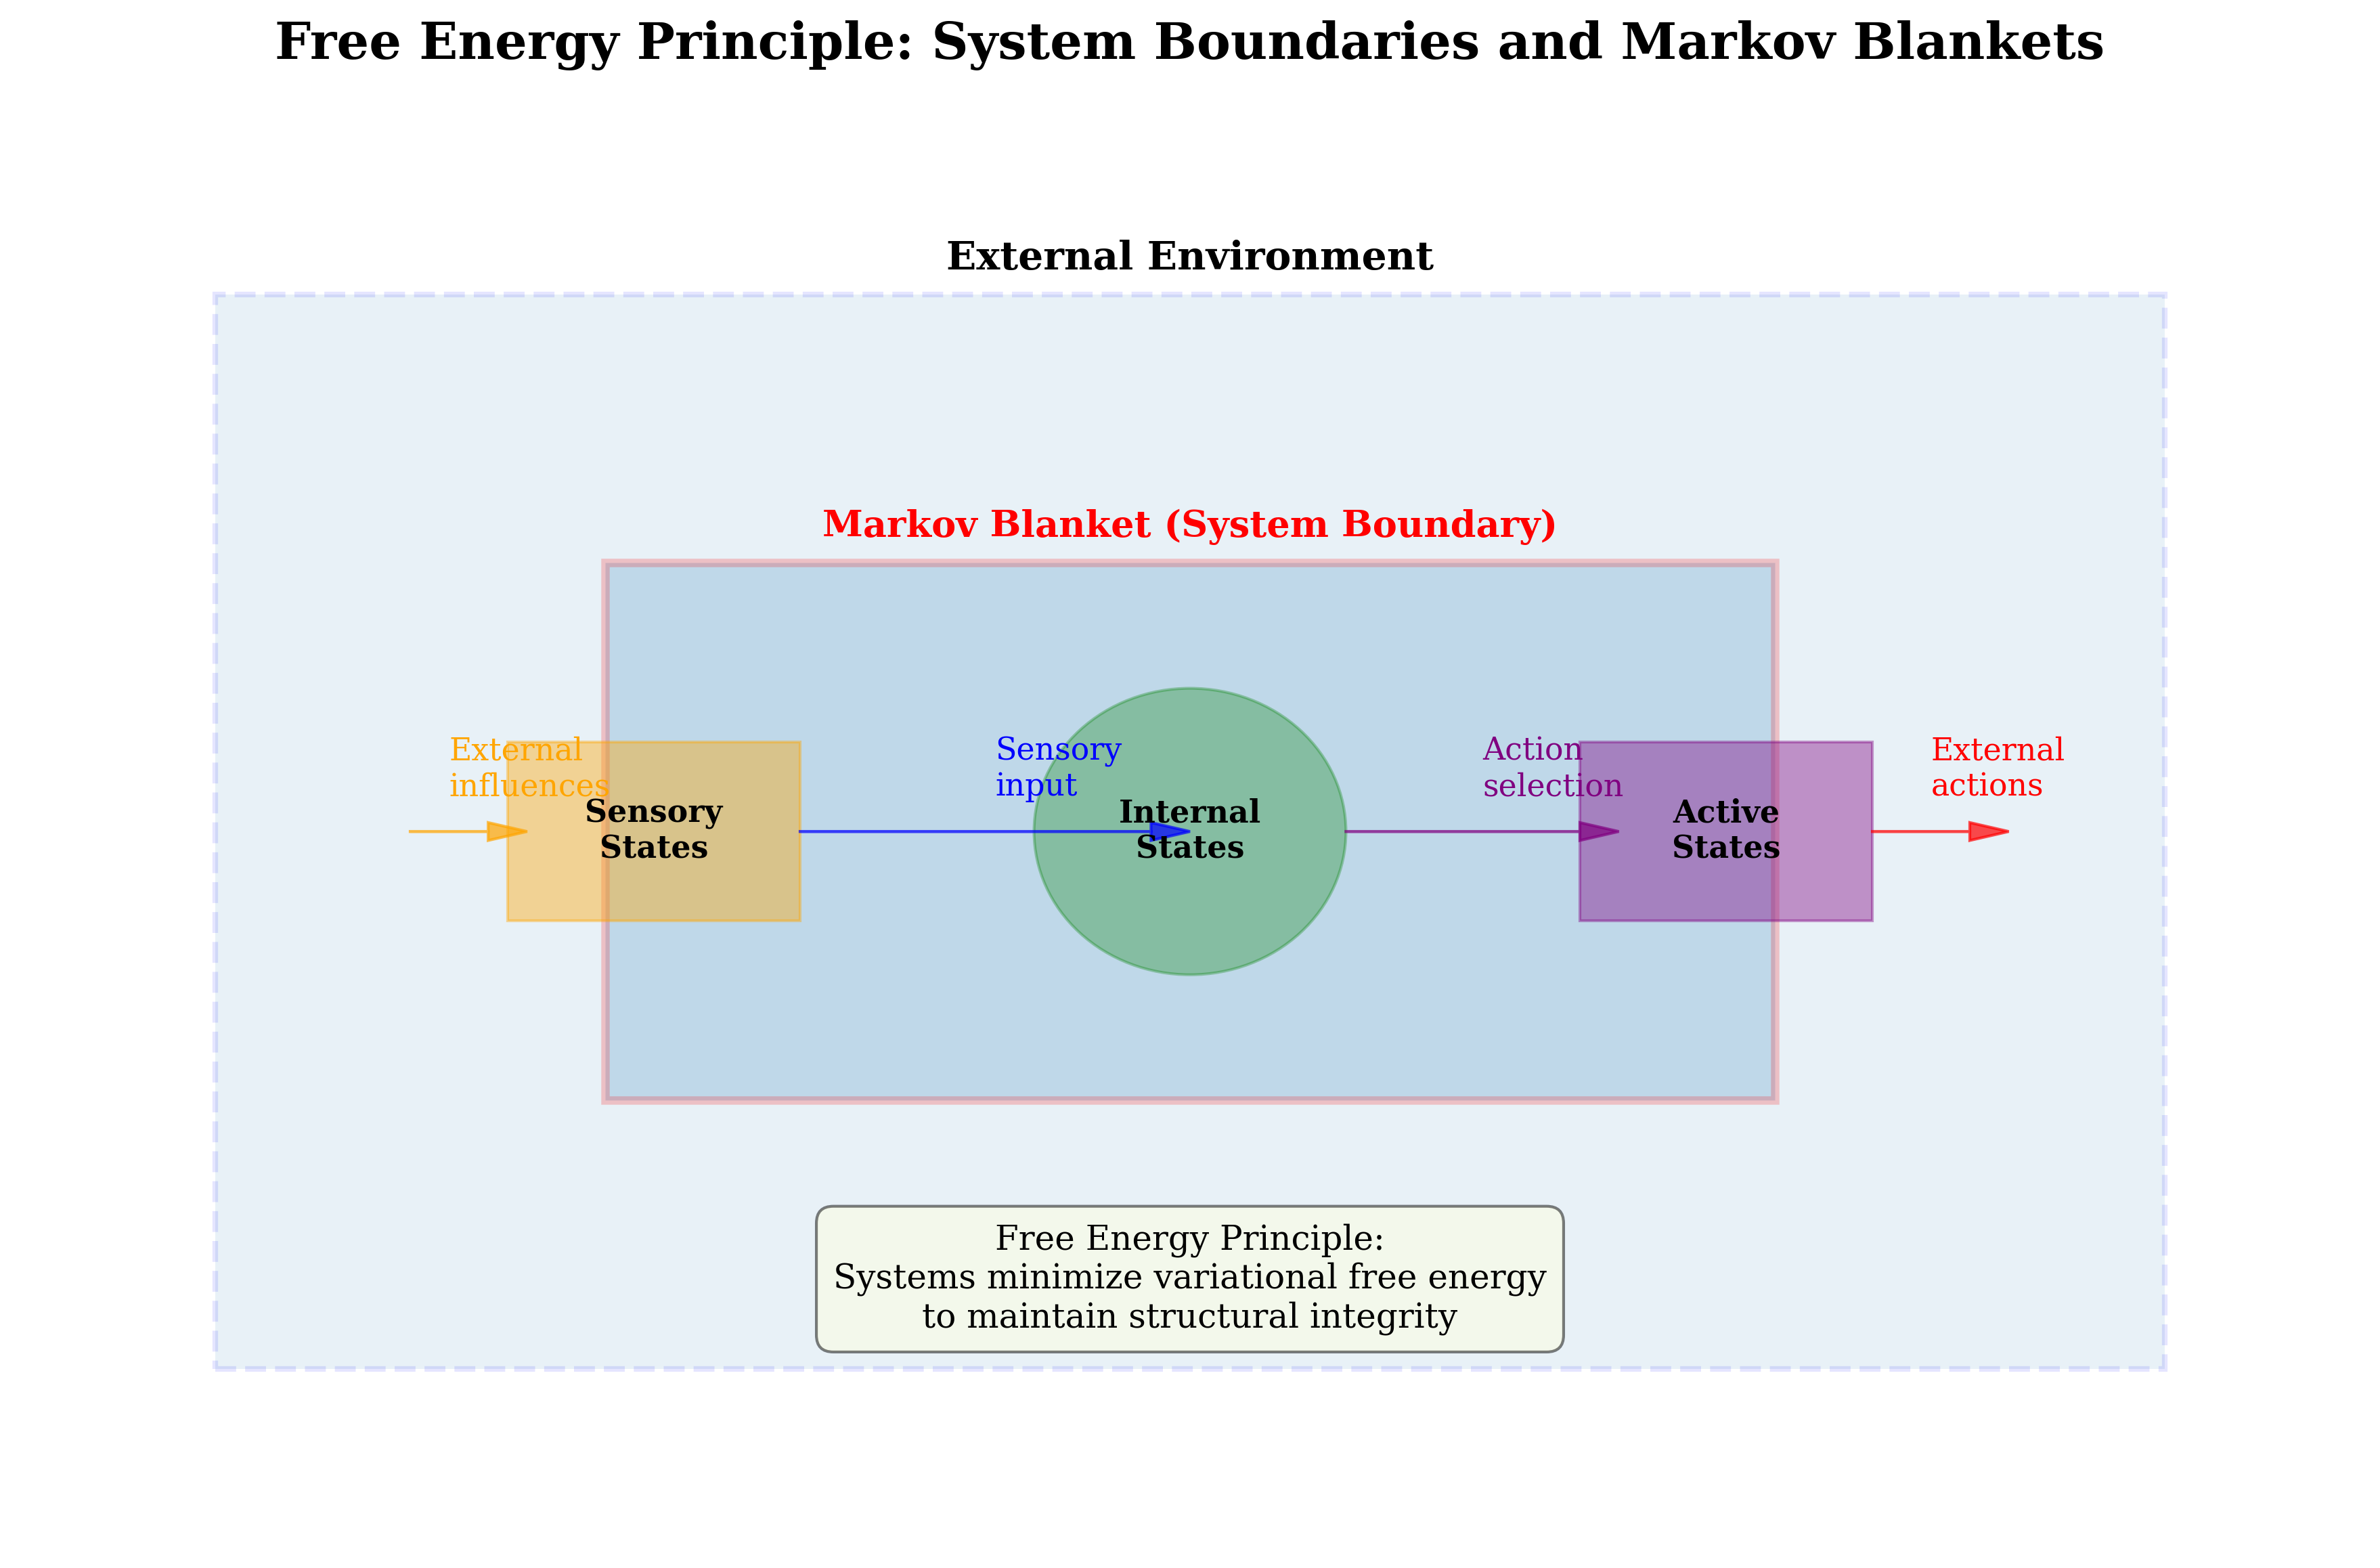
\includegraphics[width=0.8\textwidth]{../figures/fep_system_boundaries.png}
\caption{Free Energy Principle system boundaries showing Markov blanket separating internal and external states. The Markov blanket defines the boundary between a system (internal states) and its environment (external states) through sensory and active states. Systems maintain their structure by minimizing variational free energy $\mathcal{F}[q]$, which bounds surprise.}
\label{fig:fep_system_boundaries}
\end{figure}

\subsubsection{Variational Free Energy}\label{variational-free-energy}

The Variational Free Energy bounds the surprise:

\begin{equation}
\mathcal{F}[q] = \mathbb{E}_{q(s)}[\log q(s) - \log p(s,o)]
\label{eq:variational_free_energy}
\end{equation}

Systems self-organize by minimizing free energy:

\begin{equation}
\dot{\phi} = -\frac{\partial \mathcal{F}}{\partial \phi}
\label{eq:self_organization}
\end{equation}

Where \(\phi) represents system parameters that can be controlled.

\begin{figure}[h]
\centering
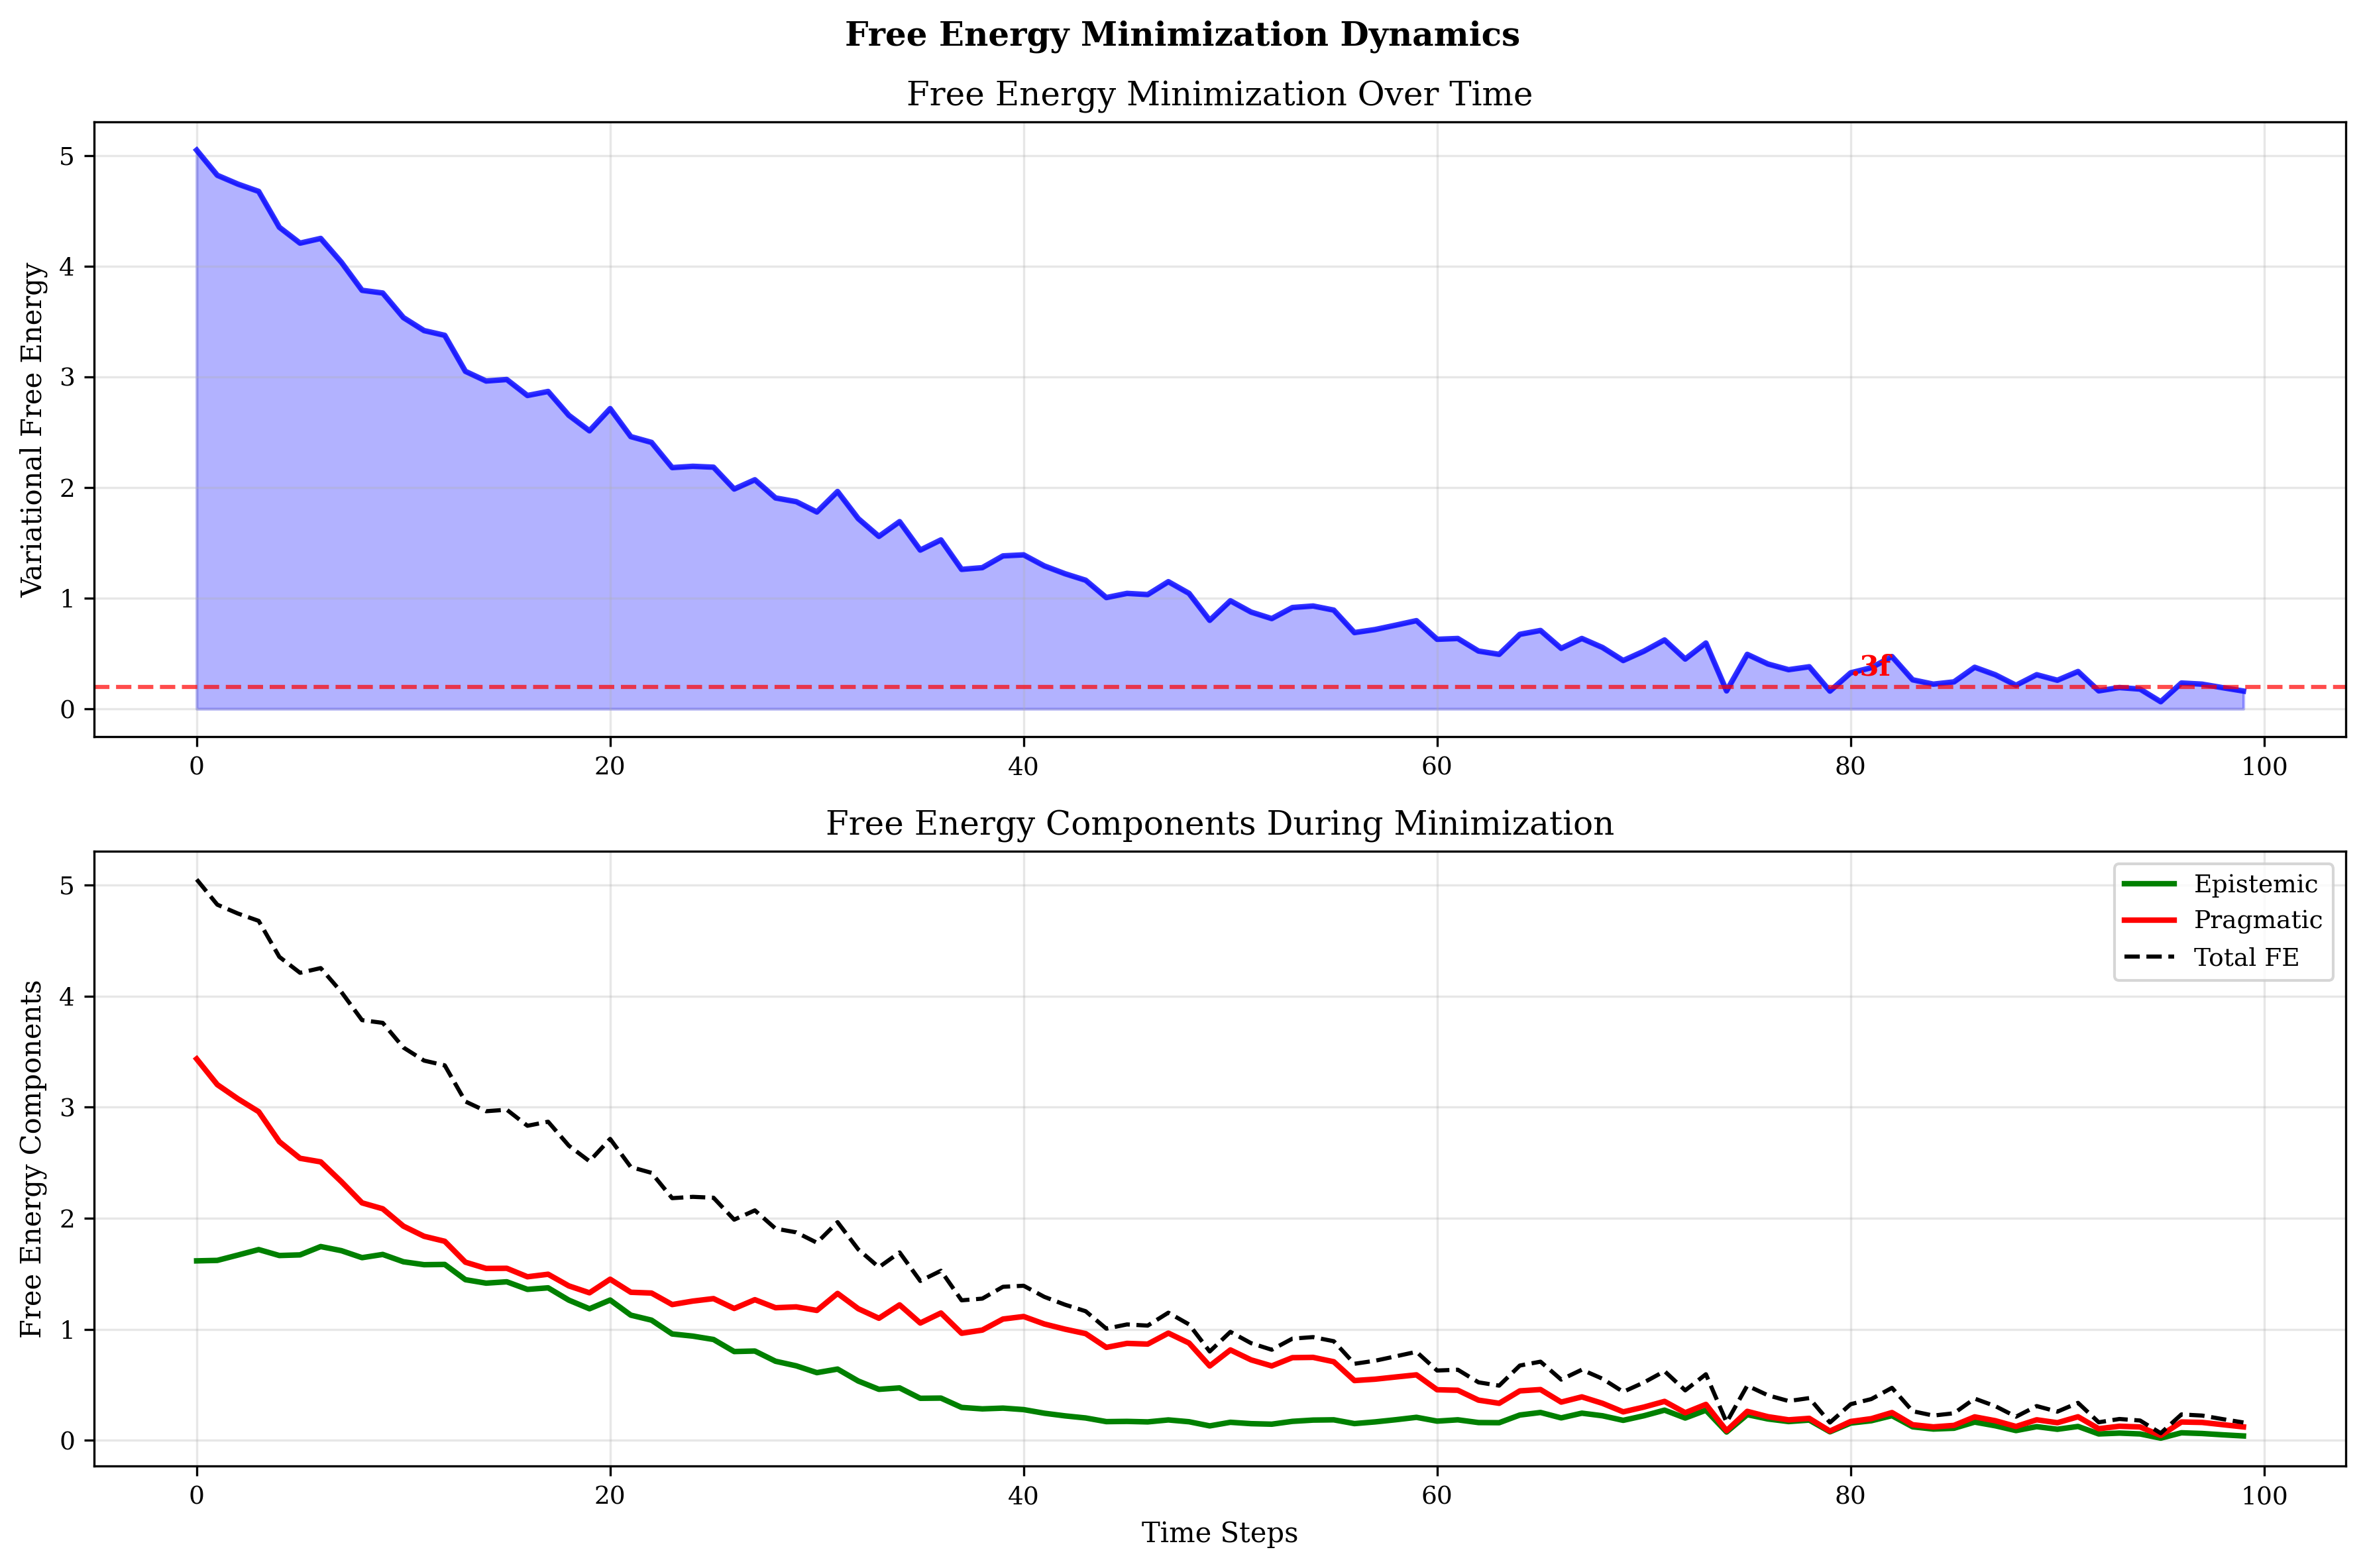
\includegraphics[width=0.8\textwidth]{../figures/free_energy_dynamics.png}
\caption{Free energy minimization dynamics showing convergence over time and epistemic/pragmatic components. The trajectory shows how variational free energy $\mathcal{F}[q]$ decreases over time as the system updates its beliefs and actions.}
\label{fig:free_energy_dynamics}
\end{figure}

\subsection{Expected Free Energy Formulation}\label{sec:efe_formulation}

The Expected Free Energy (EFE) combines epistemic and pragmatic
components in a unified formalism:

\begin{equation}
\mathcal{F}(\pi) = \mathbb{E}_{q(s_\tau)}[\log q(s_\tau) - \log p(s_\tau \mid \pi)] + \mathbb{E}_{q(o_\tau)}[\log p(o_\tau \mid s_\tau) + \log p(s_\tau) - \log q(s_\tau)]
\label{eq:efe}
\end{equation}

\subsubsection{Epistemic-Pragmatic
Decomposition}\label{epistemic-pragmatic-decomposition}

The EFE decomposes into two fundamental terms:

\textbf{Epistemic Value (Information Gain):}

\begin{equation}
H[Q(\pi)] = \mathbb{E}_{q(s_\tau)}[\log q(s_\tau) - \log p(s_\tau \mid \pi)]
\label{eq:epistemic_component}
\end{equation}

This term (Equation \eqref{eq:epistemic_component}) is minimized when
executing policy \(\pi) reduces uncertainty about hidden states.

\textbf{Pragmatic Value (Goal Achievement):}

\begin{equation}
G(\pi) = \mathbb{E}_{q(o_\tau)}[\log p(o_\tau \mid s_\tau) + \log p(s_\tau) - \log q(s_\tau)]
\label{eq:pragmatic_component}
\end{equation}

This term (Equation \eqref{eq:pragmatic_component}) measures goal
achievement through preferred observations.

\begin{figure}[h]
\centering
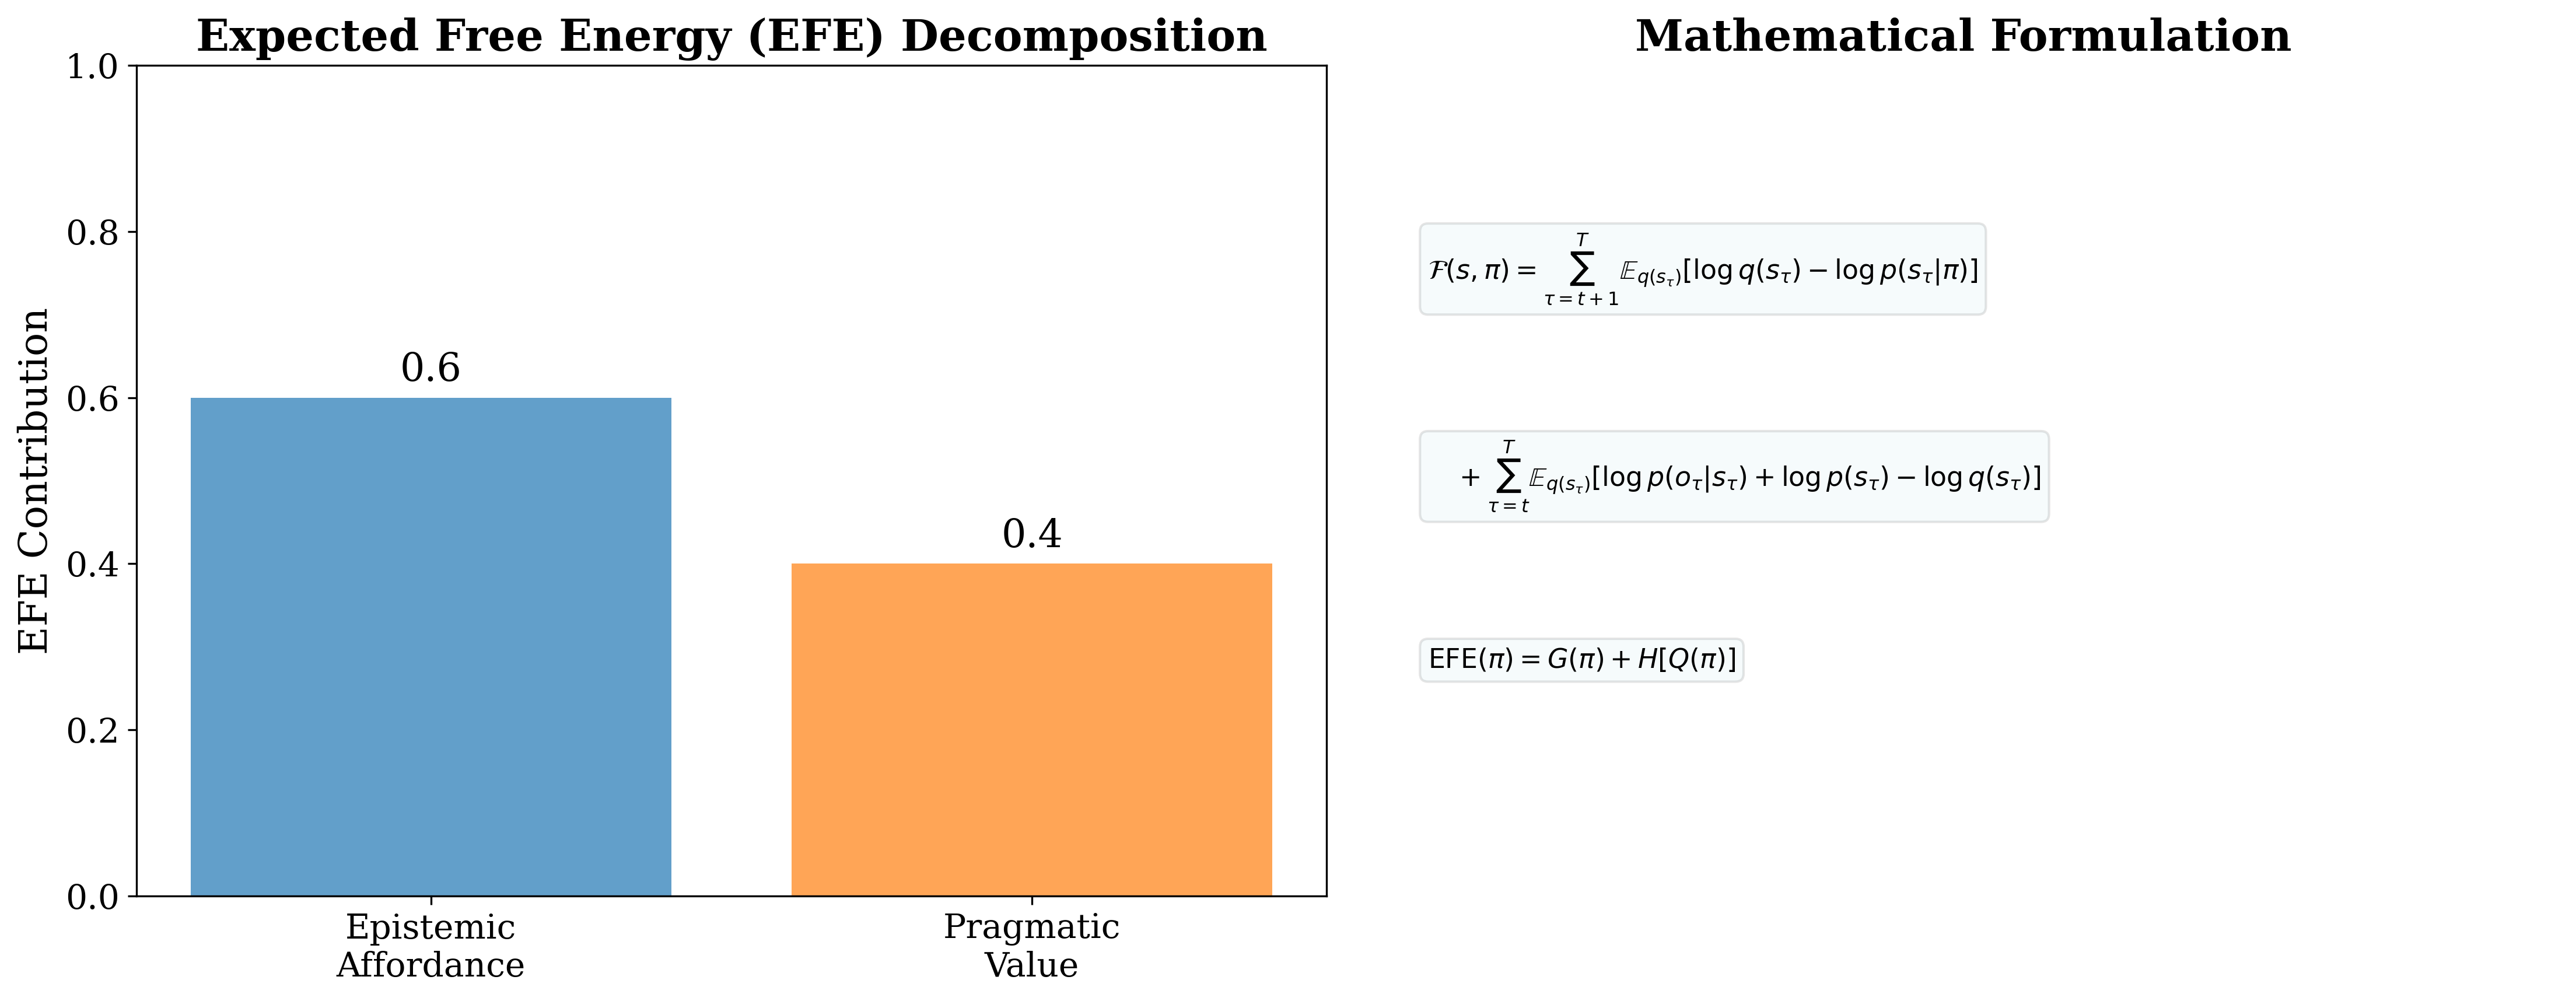
\includegraphics[width=0.8\textwidth]{../figures/efe_decomposition.png}
\caption{Expected Free Energy (EFE) decomposition into epistemic and pragmatic components (Equation \eqref{eq:efe}). The EFE $\mathcal{F}(\pi)$ combines epistemic affordance $H[Q(\pi)]$ (information gain) and pragmatic value $G(\pi)$ (goal achievement), enabling systematic analysis of how agents balance exploration and exploitation.}
\label{fig:efe_decomposition}
\end{figure}

\subsubsection{Perception-Action Loop}\label{perception-action-loop}

Active Inference implements a continuous cycle where agents update
beliefs and select actions to minimize expected free energy:

\begin{figure}[h]
\centering
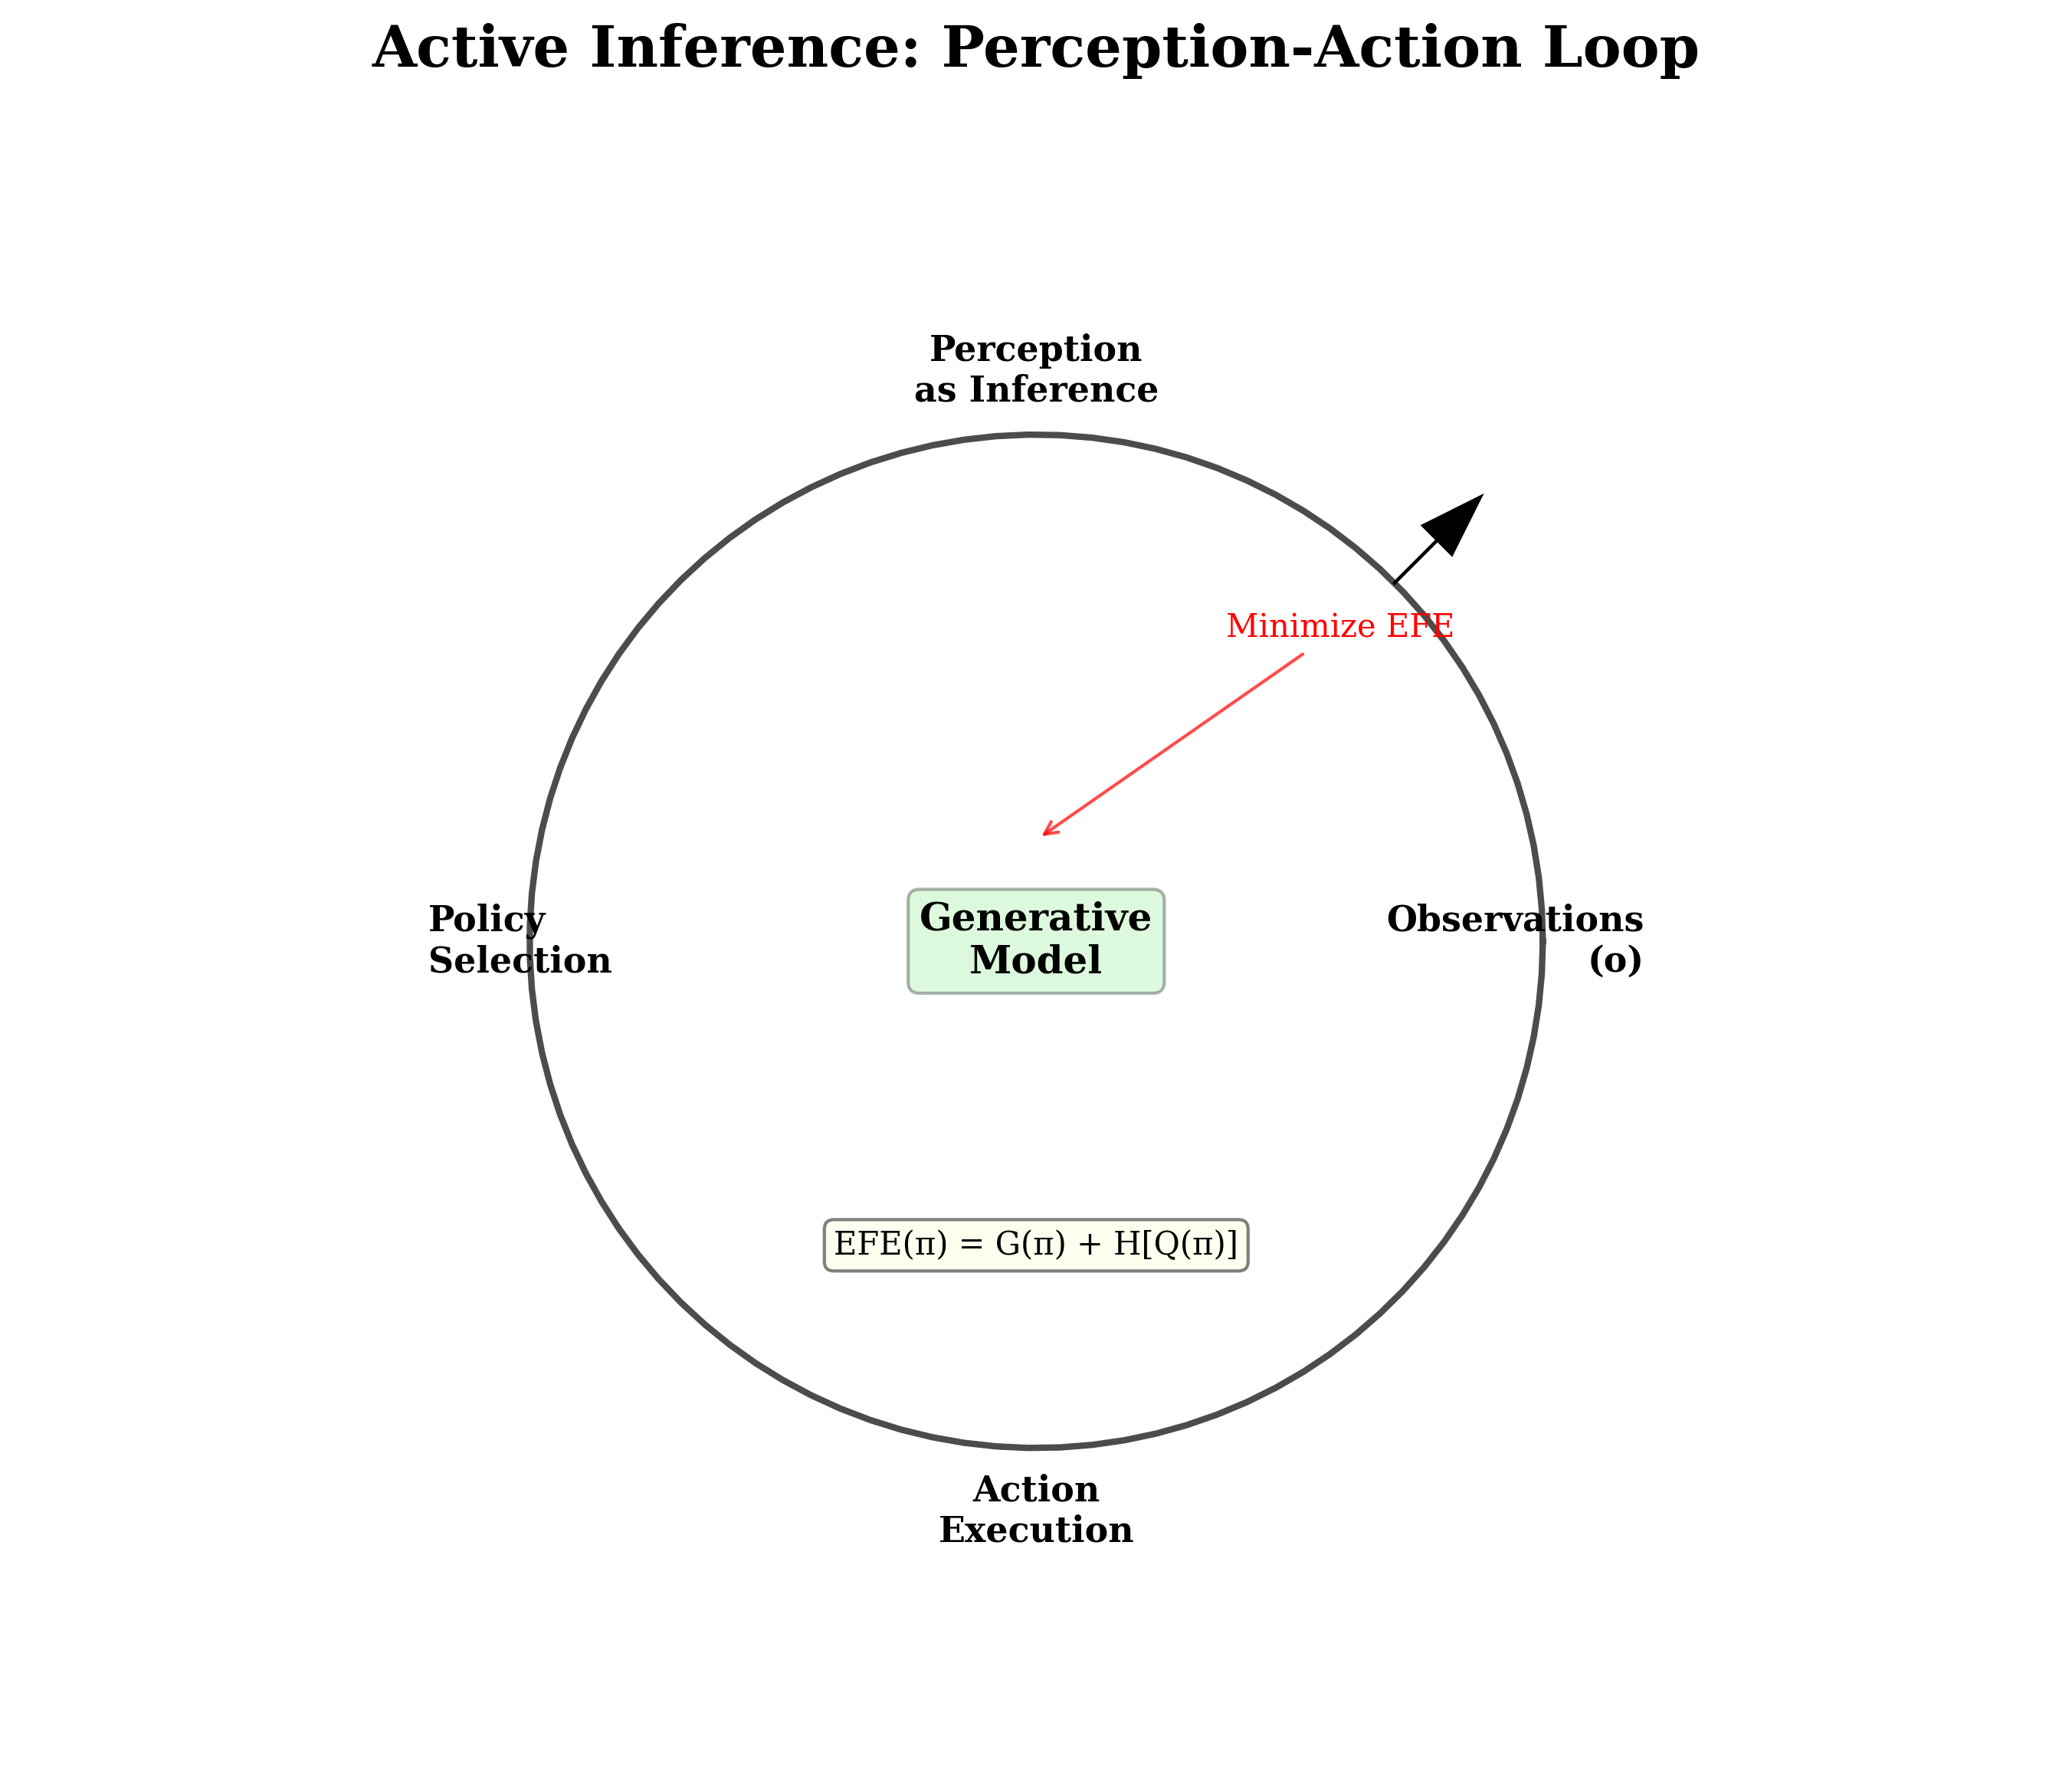
\includegraphics[width=0.8\textwidth]{../figures/perception_action_loop.png}
\caption{Active Inference perception-action loop showing how perception drives action through EFE minimization (Equation \eqref{eq:efe}). The cycle consists of: (1) Observation of sensory data; (2) Bayesian inference updating posterior beliefs $q(s)$ about hidden states; (3) Policy evaluation computing EFE $\mathcal{F}(\pi)$ for candidate actions; (4) Action selection minimizing EFE; (5) Action execution generating new observations.}
\label{fig:perception_action_loop}
\end{figure}

\subsection{Generative Model Specification}\label{sec:generative_model}

Active Inference agents operate through generative models defined by
four core matrices. The specification of these matrices transforms
framework design from an external constraint into an internal research
question.

\subsubsection{Matrix A: Observation
Likelihoods}\label{matrix-a-observation-likelihoods}

Defines how hidden states generate observations:

\begin{equation}
A = [a_{ij}] \quad a_{ij} = P(o_i \mid s_j)
\label{eq:matrix_a}
\end{equation}

\textbf{Properties:}

\begin{itemize}
\tightlist
\item
  Each column sums to 1 (valid probability distribution)
\item
  Rows represent observation modalities
\item
  Columns represent hidden state conditions
\item
  Diagonal dominance indicates reliable observations
\end{itemize}

\subsubsection{Matrix B: State
Transitions}\label{matrix-b-state-transitions}

Defines how actions influence state changes:

\begin{equation}
B = [b_{ijk}] \quad b_{ijk} = P(s_j \mid s_i, a_k)
\label{eq:matrix_b}
\end{equation}

\textbf{Structure:} 3D tensor with dimensions
\(\text{states} \times \text{states} \times \text{actions}\), where each
action defines a transition matrix.

\subsubsection{Matrix C: Preferences}\label{matrix-c-preferences}

Defines desired outcomes (the pragmatic landscape):

\begin{equation}
C = [c_i] \quad c_i = \log P(o_i)
\label{eq:matrix_c}
\end{equation}

\textbf{Interpretation:}

\begin{itemize}
\tightlist
\item
  Positive values: preferred observations
\item
  Negative values: avoided observations
\item
  Magnitude indicates strength of preference
\end{itemize}

\subsubsection{Matrix D: Prior Beliefs}\label{matrix-d-prior-beliefs}

Defines initial state beliefs:

\begin{equation}
D = [d_i] \quad d_i = P(s_i)
\label{eq:matrix_d}
\end{equation}

\textbf{Role:} Represents initial beliefs before observation, encoding
innate biases or learned priors.

\begin{figure}[h]
\centering
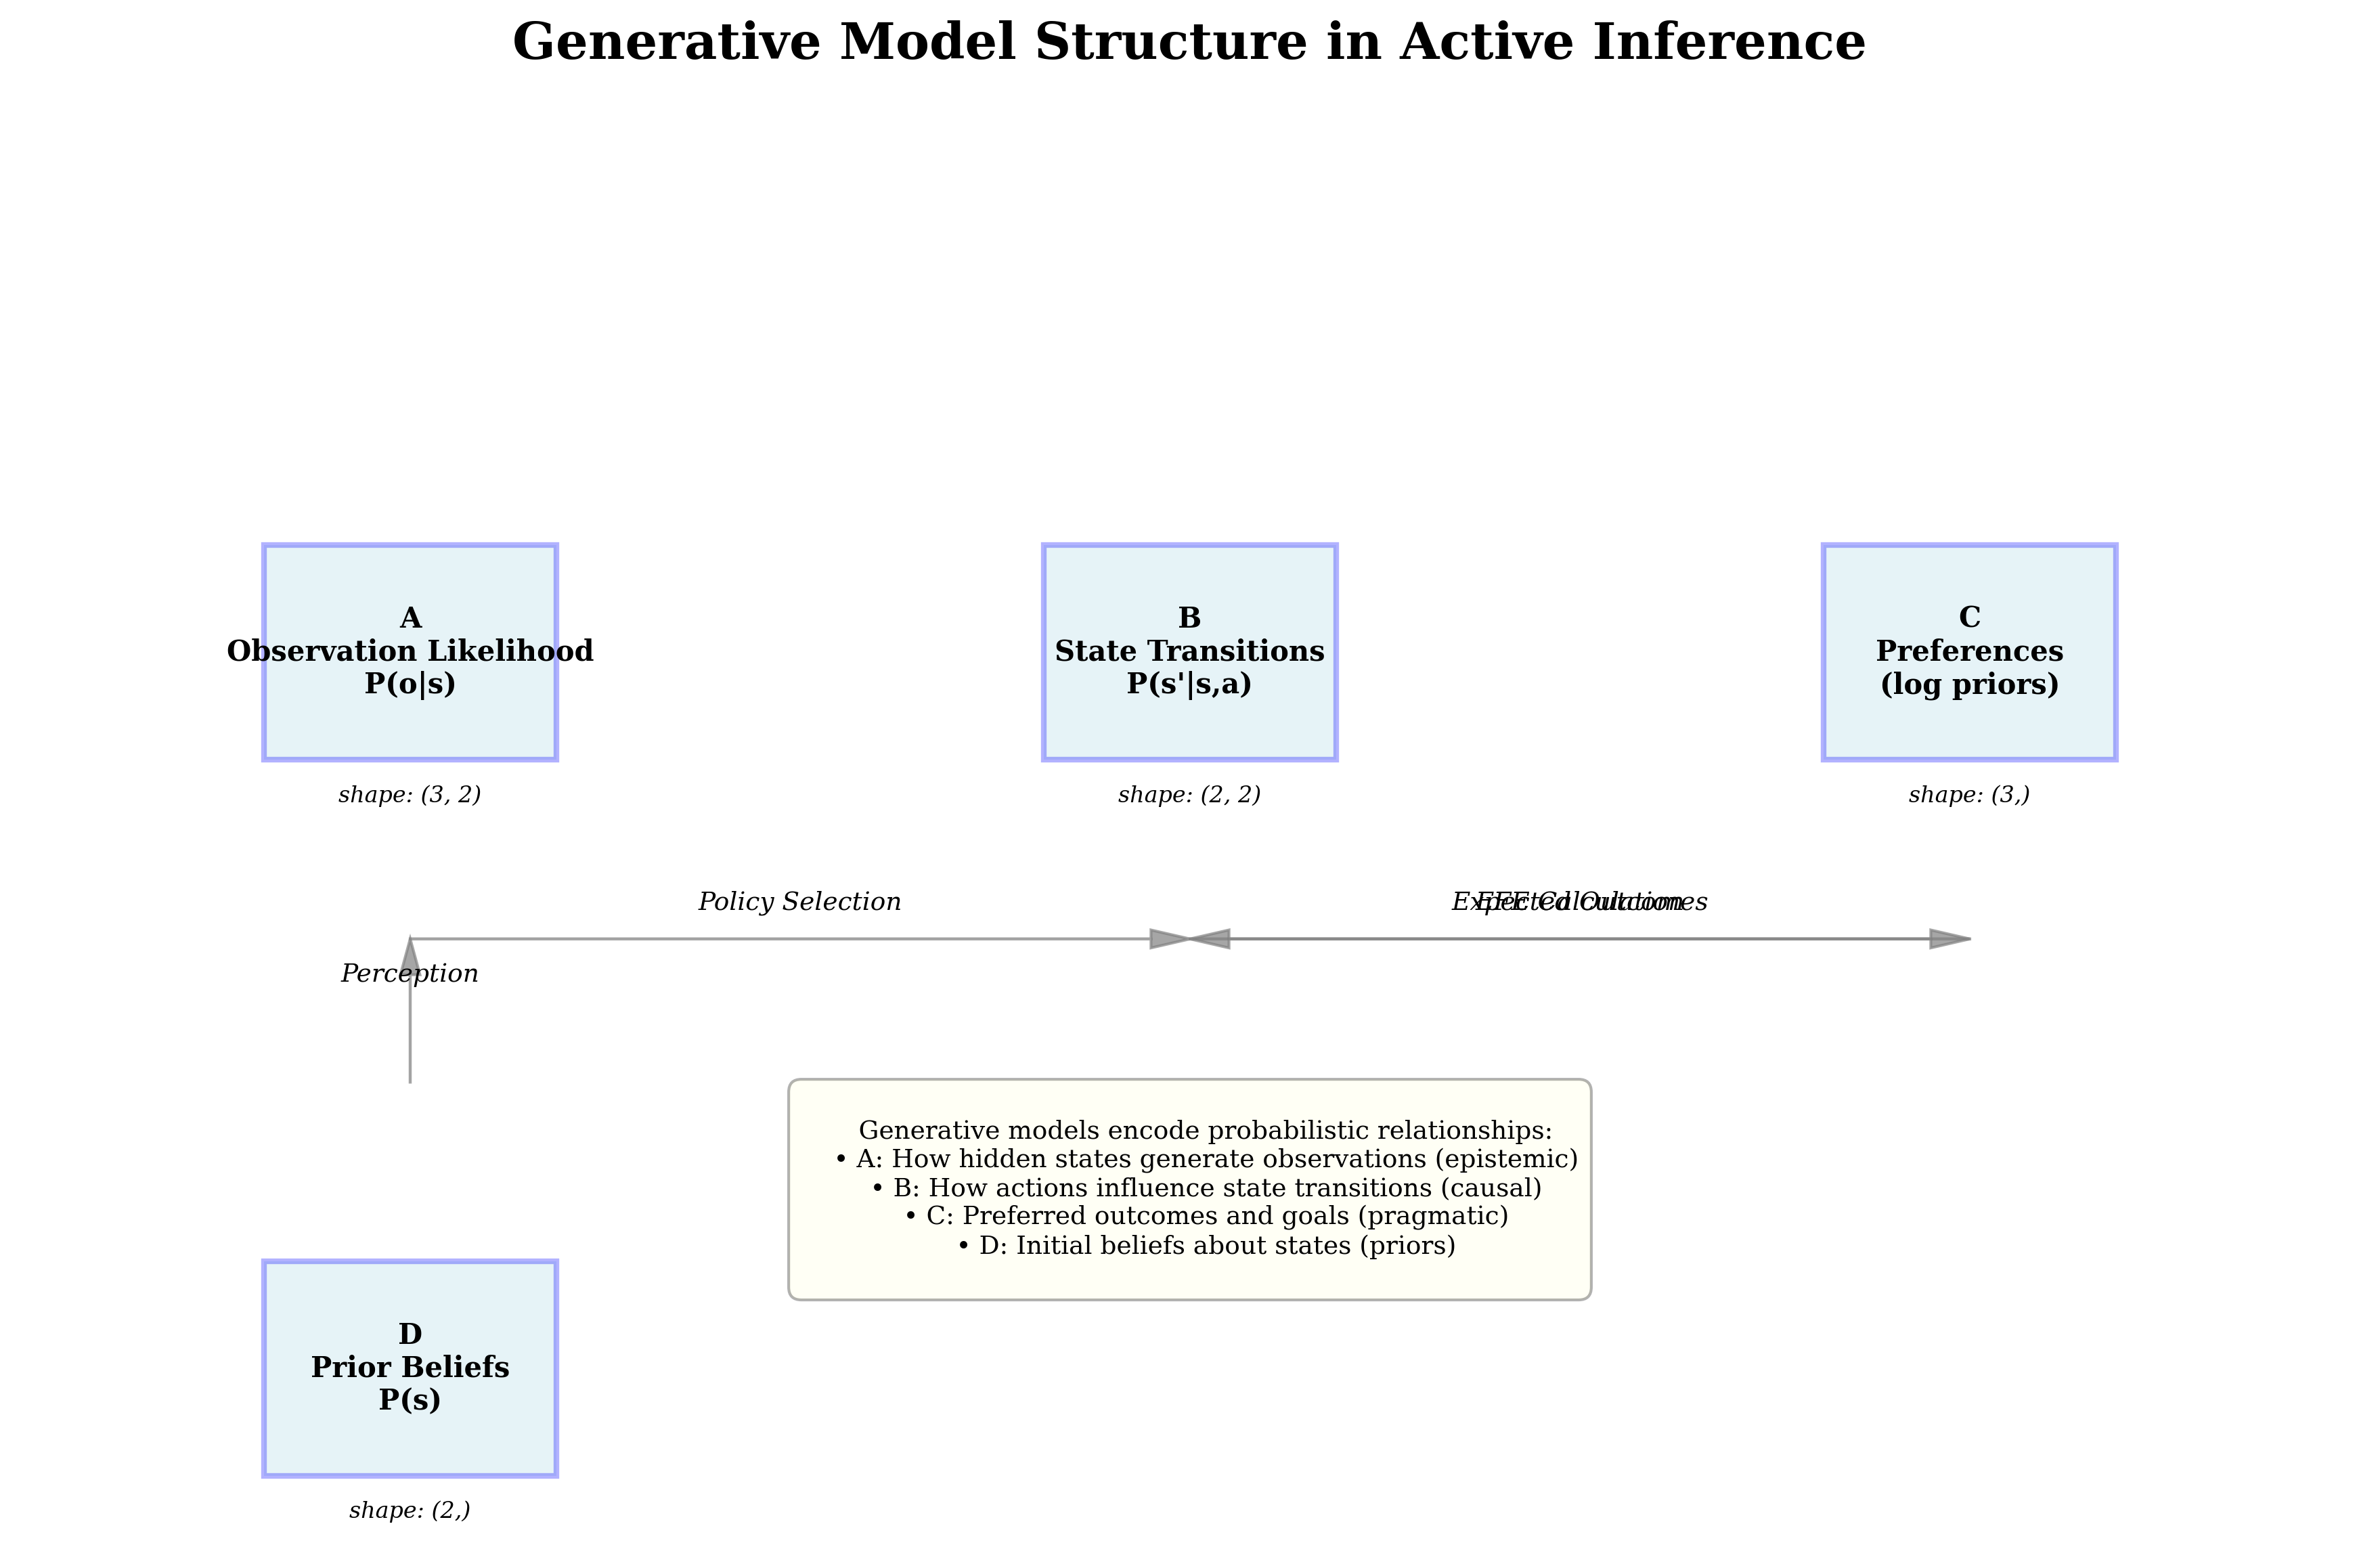
\includegraphics[width=0.8\textwidth]{../figures/generative_model_structure.png}
\caption{Structure of generative models in Active Inference showing $A$, $B$, $C$, $D$ matrices and their relationships. Matrix $A$ (Equation \eqref{eq:matrix_a}) defines observation likelihoods. Matrix $B$ (Equation \eqref{eq:matrix_b}) defines state transitions. Matrix $C$ (Equation \eqref{eq:matrix_c}) defines preferences. Matrix $D$ (Equation \eqref{eq:matrix_d}) defines prior beliefs.}
\label{fig:generative_model_structure}
\end{figure}

\subsection{Meta-Epistemic and Meta-Pragmatic
Aspects}\label{sec:meta_aspects}

Active Inference operates at a fundamentally meta-level that
distinguishes it from traditional decision-making algorithms. Rather
than simply providing another method for selecting actions given fixed
observation models and reward functions, Active Inference allows
researchers to specify the very frameworks within which cognition
occurs.

\subsubsection{Meta-Epistemic Dimension}\label{meta-epistemic-dimension}

Active Inference allows modelers to specify epistemic frameworks through
matrices \(A\), \(B\), and \(D\):

\begin{itemize}
\tightlist
\item
  \textbf{Matrix \(A\):} Defines what can be known about the world and
  how reliably observations indicate underlying states
\item
  \textbf{Matrix \(D\):} Sets initial assumptions about the world's
  structure
\item
  \textbf{Matrix \(B\):} Specifies causal relationships and how actions
  influence state changes
\end{itemize}

Through these specifications, researchers define not just current
beliefs, but the epistemological boundaries of cognition
itself---determining what knowledge is possible, how evidence
accumulates, and what causal structures are assumed.

\subsubsection{Meta-Pragmatic Dimension}\label{meta-pragmatic-dimension}

Beyond epistemic specification, Active Inference supports meta-pragmatic
modeling through matrix \(C\), which defines preference priors. Unlike
traditional reinforcement learning where rewards are externally
specified, Active Inference allows modelers to specify pragmatic
landscapes---what constitutes ``value'' for the agent---creating
opportunities to explore how different value systems shape cognition and
behavior.

\begin{figure}[h]
\centering
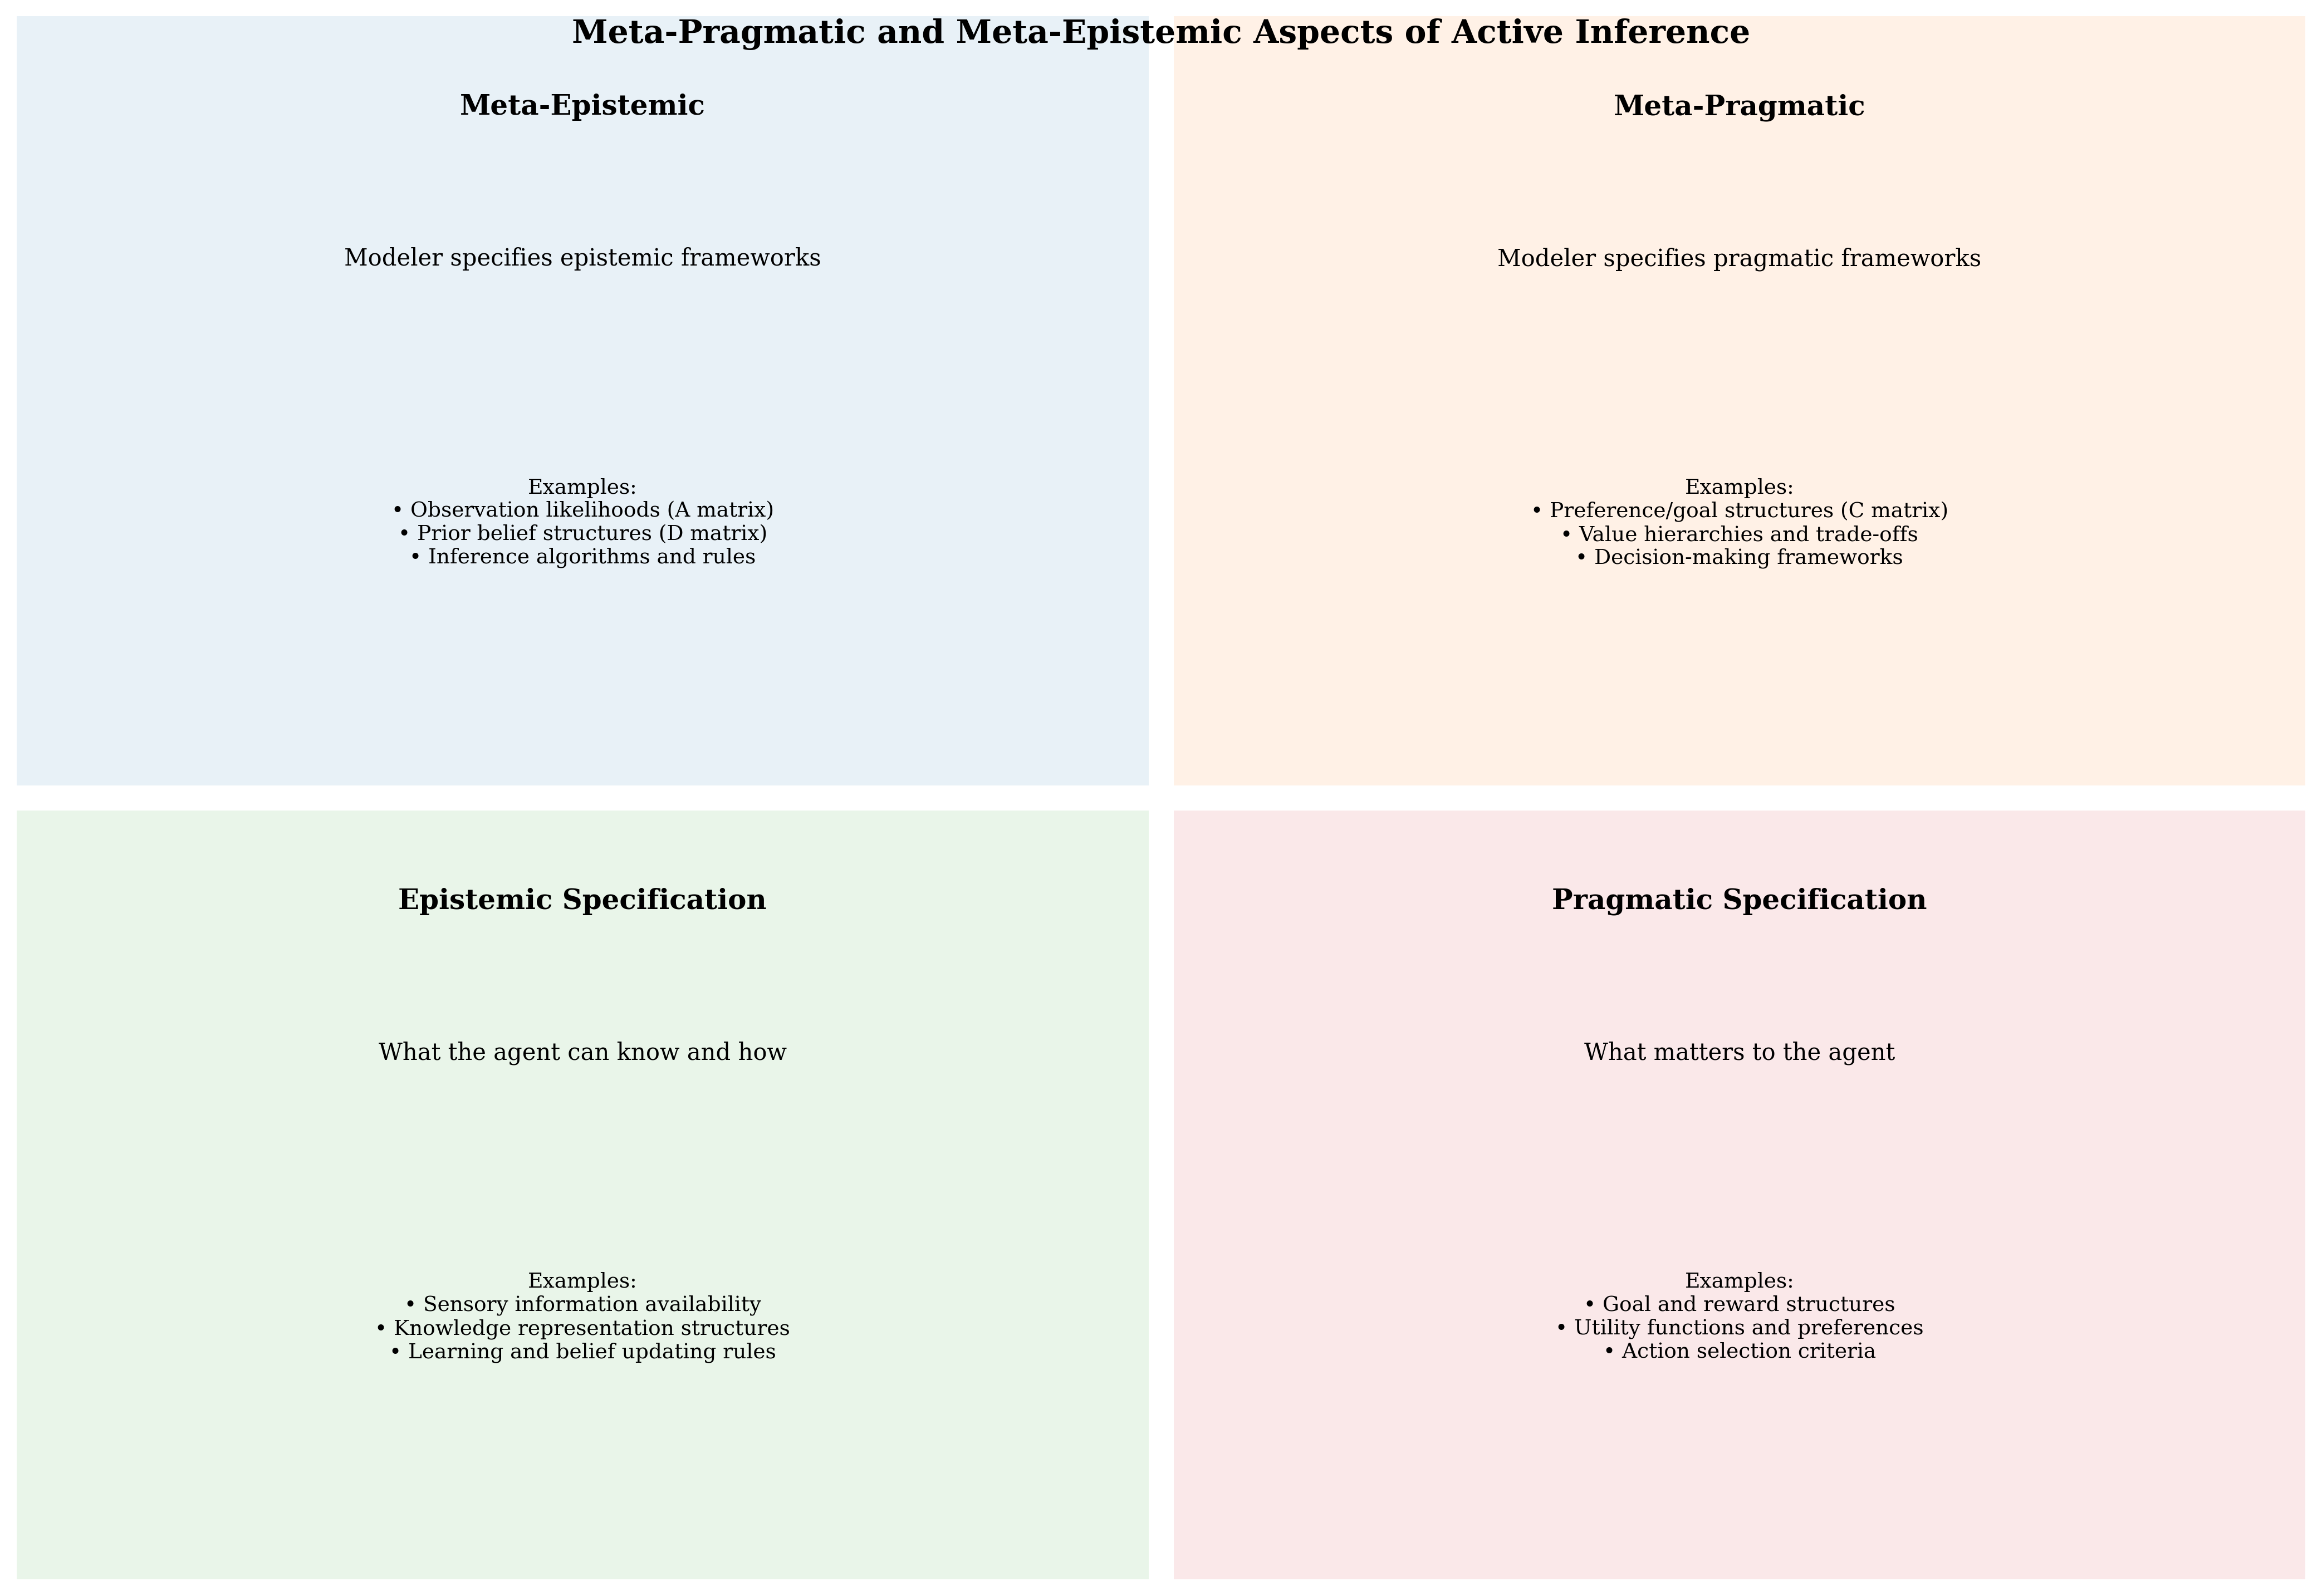
\includegraphics[width=0.8\textwidth]{../figures/meta_level_concepts.png}
\caption{Meta-pragmatic and meta-epistemic aspects showing modeler specification power. The meta-epistemic dimension enables specification of knowledge acquisition frameworks through matrices $A$, $B$, and $D$. The meta-pragmatic dimension enables specification of value landscapes through matrix $C$. This dual specification power makes Active Inference a meta-methodology for cognitive science.}
\label{fig:meta_level_concepts}
\end{figure}

\subsubsection{The Modeler as Architect and
Subject}\label{the-modeler-as-architect-and-subject}

The structure reveals the dual role of the Active Inference modeler:

\textbf{As Architect:}

\begin{itemize}
\tightlist
\item
  Specifies epistemic frameworks (\(A\), \(B\), \(D\) matrices)
\item
  Defines pragmatic landscapes (\(C\) matrix)
\item
  Designs cognitive architectures
\item
  Establishes boundary conditions for cognition
\end{itemize}

\textbf{As Subject:}

\begin{itemize}
\tightlist
\item
  Uses Active Inference to understand their own cognition
\item
  Applies meta-epistemic principles to knowledge acquisition
\item
  Employs meta-pragmatic frameworks for decision-making
\item
  Engages in recursive self-modeling
\end{itemize}

This dual role creates a recursive relationship where the tools used to
model others become tools for self-understanding.

\begin{figure}[h]
\centering
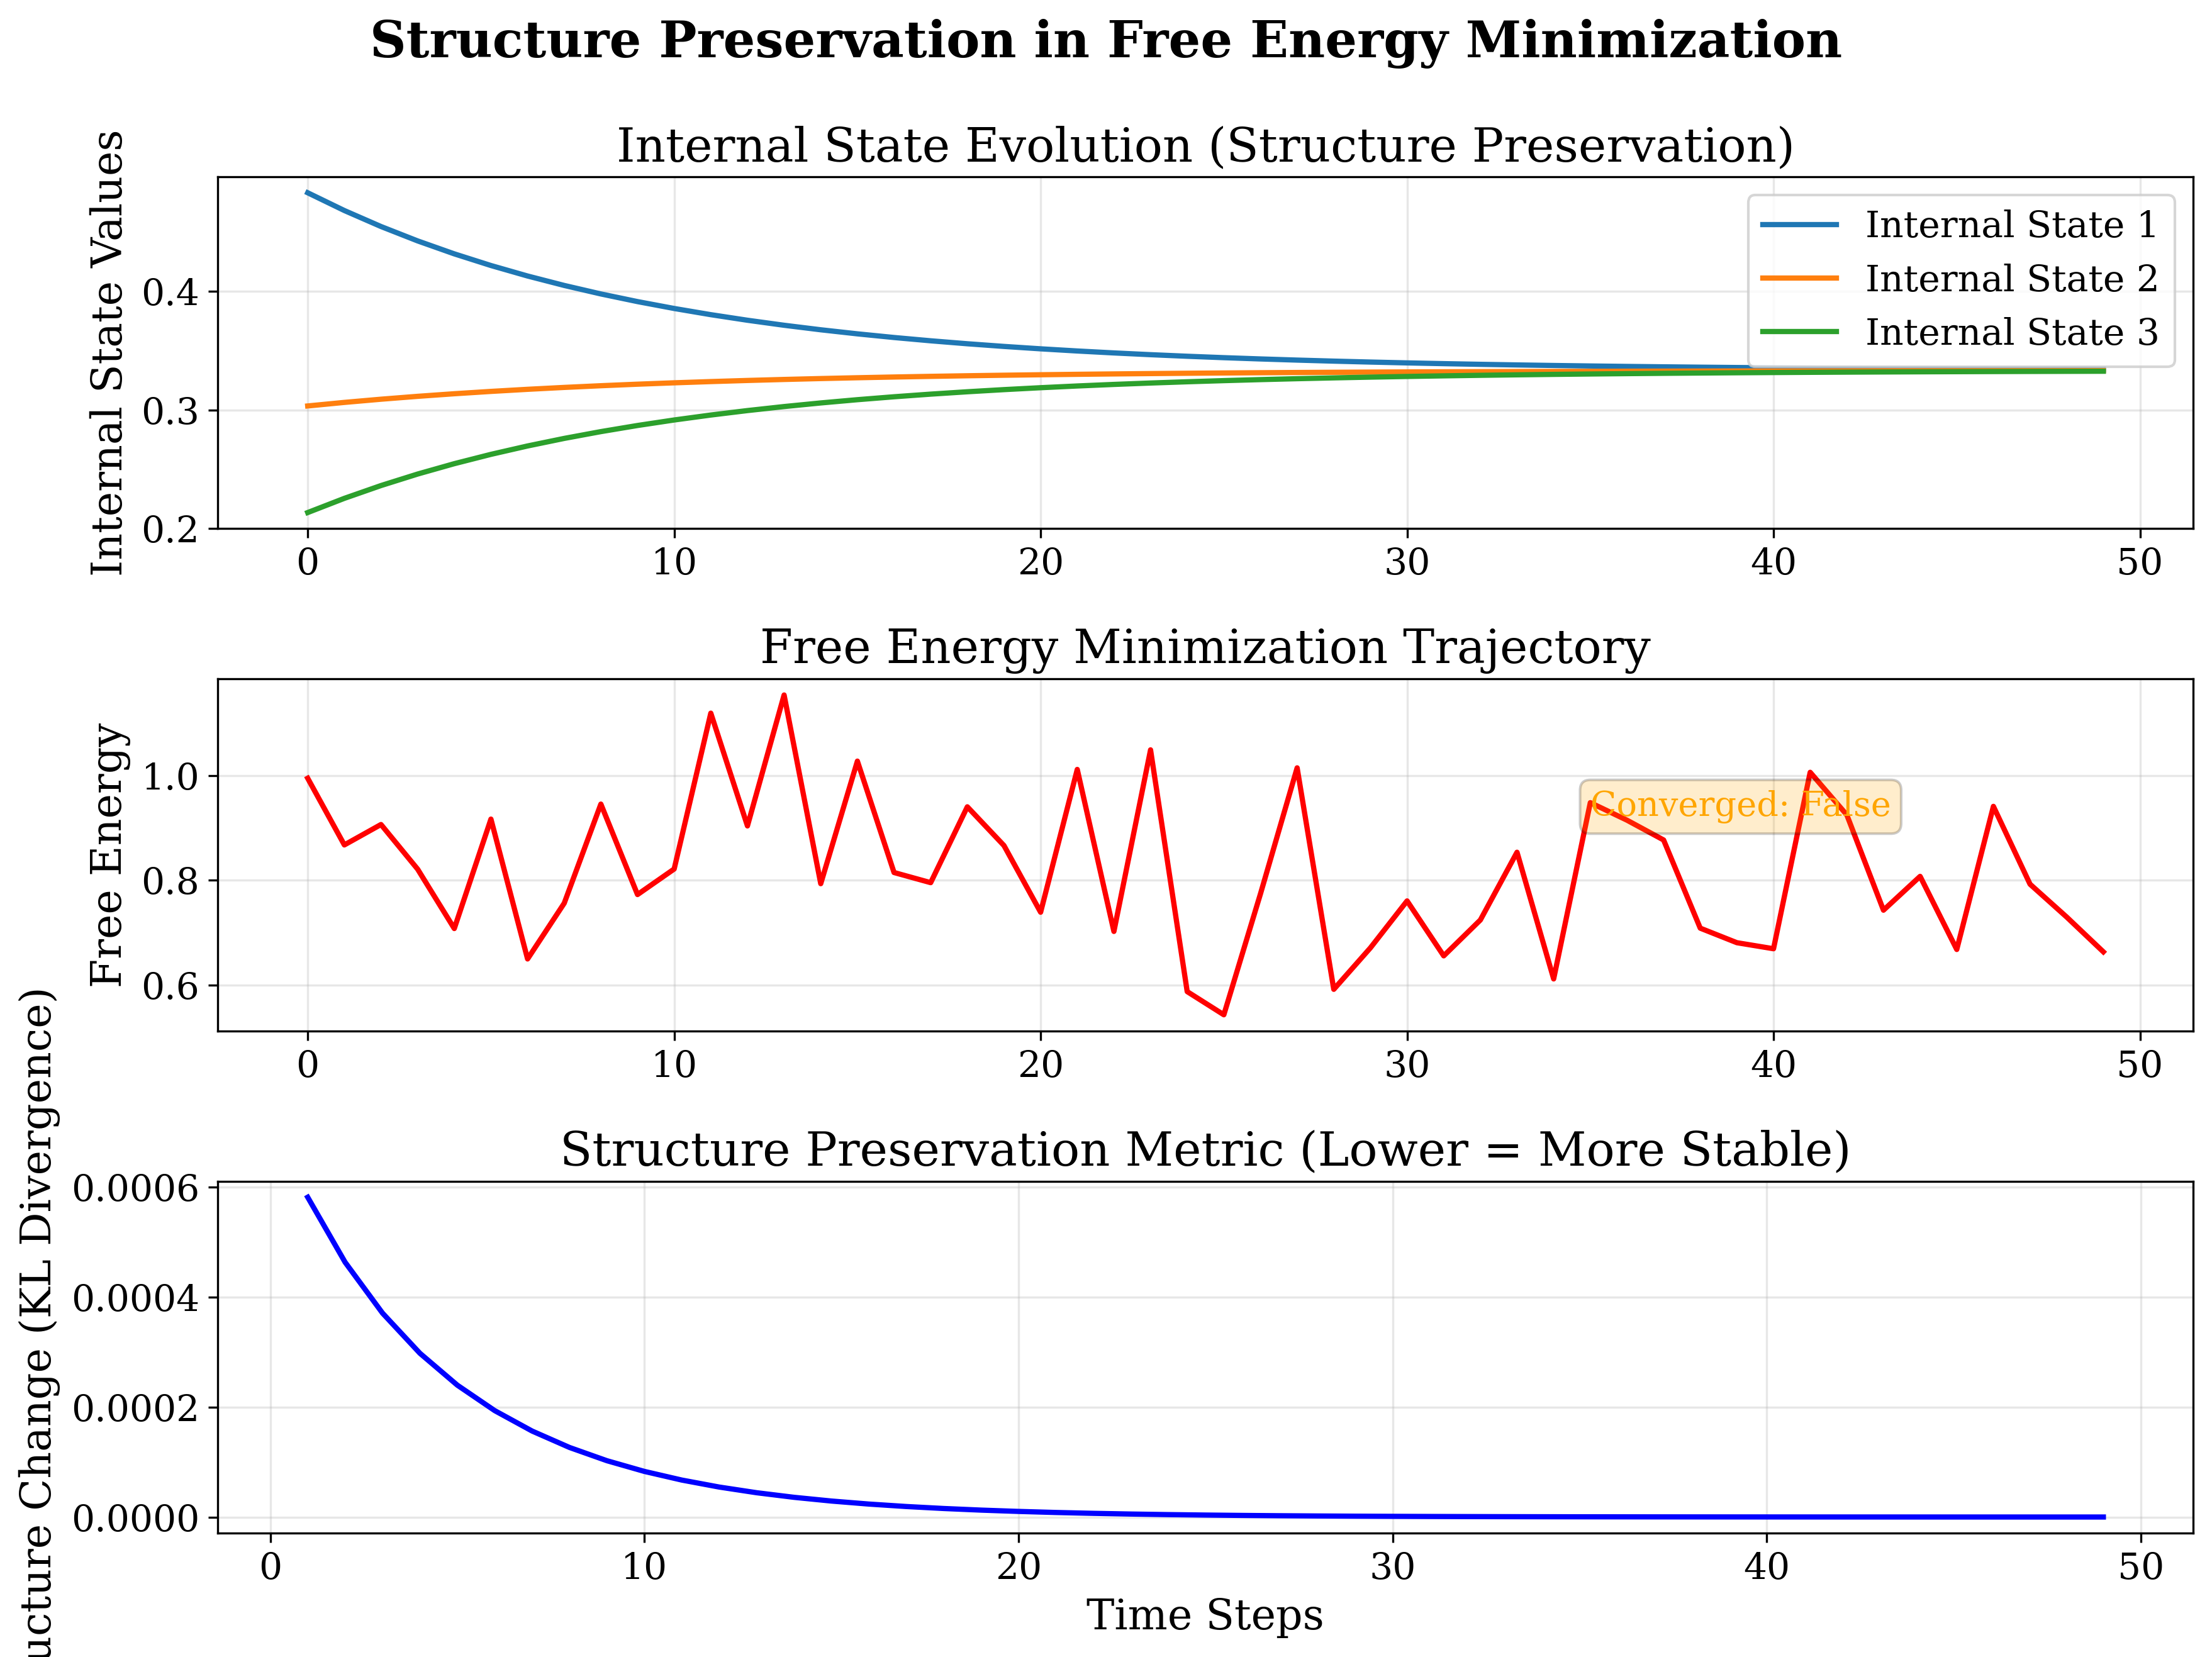
\includegraphics[width=0.8\textwidth]{../figures/structure_preservation.png}
\caption{Structure preservation dynamics showing how systems maintain internal organization through free energy minimization. Despite external perturbations and environmental changes, systems maintain stable internal states through active inference. This principle explains how biological systems, cognitive agents, and even social structures maintain their identity over time.}
\label{fig:structure_preservation}
\end{figure}

\begin{figure}[h]
\centering
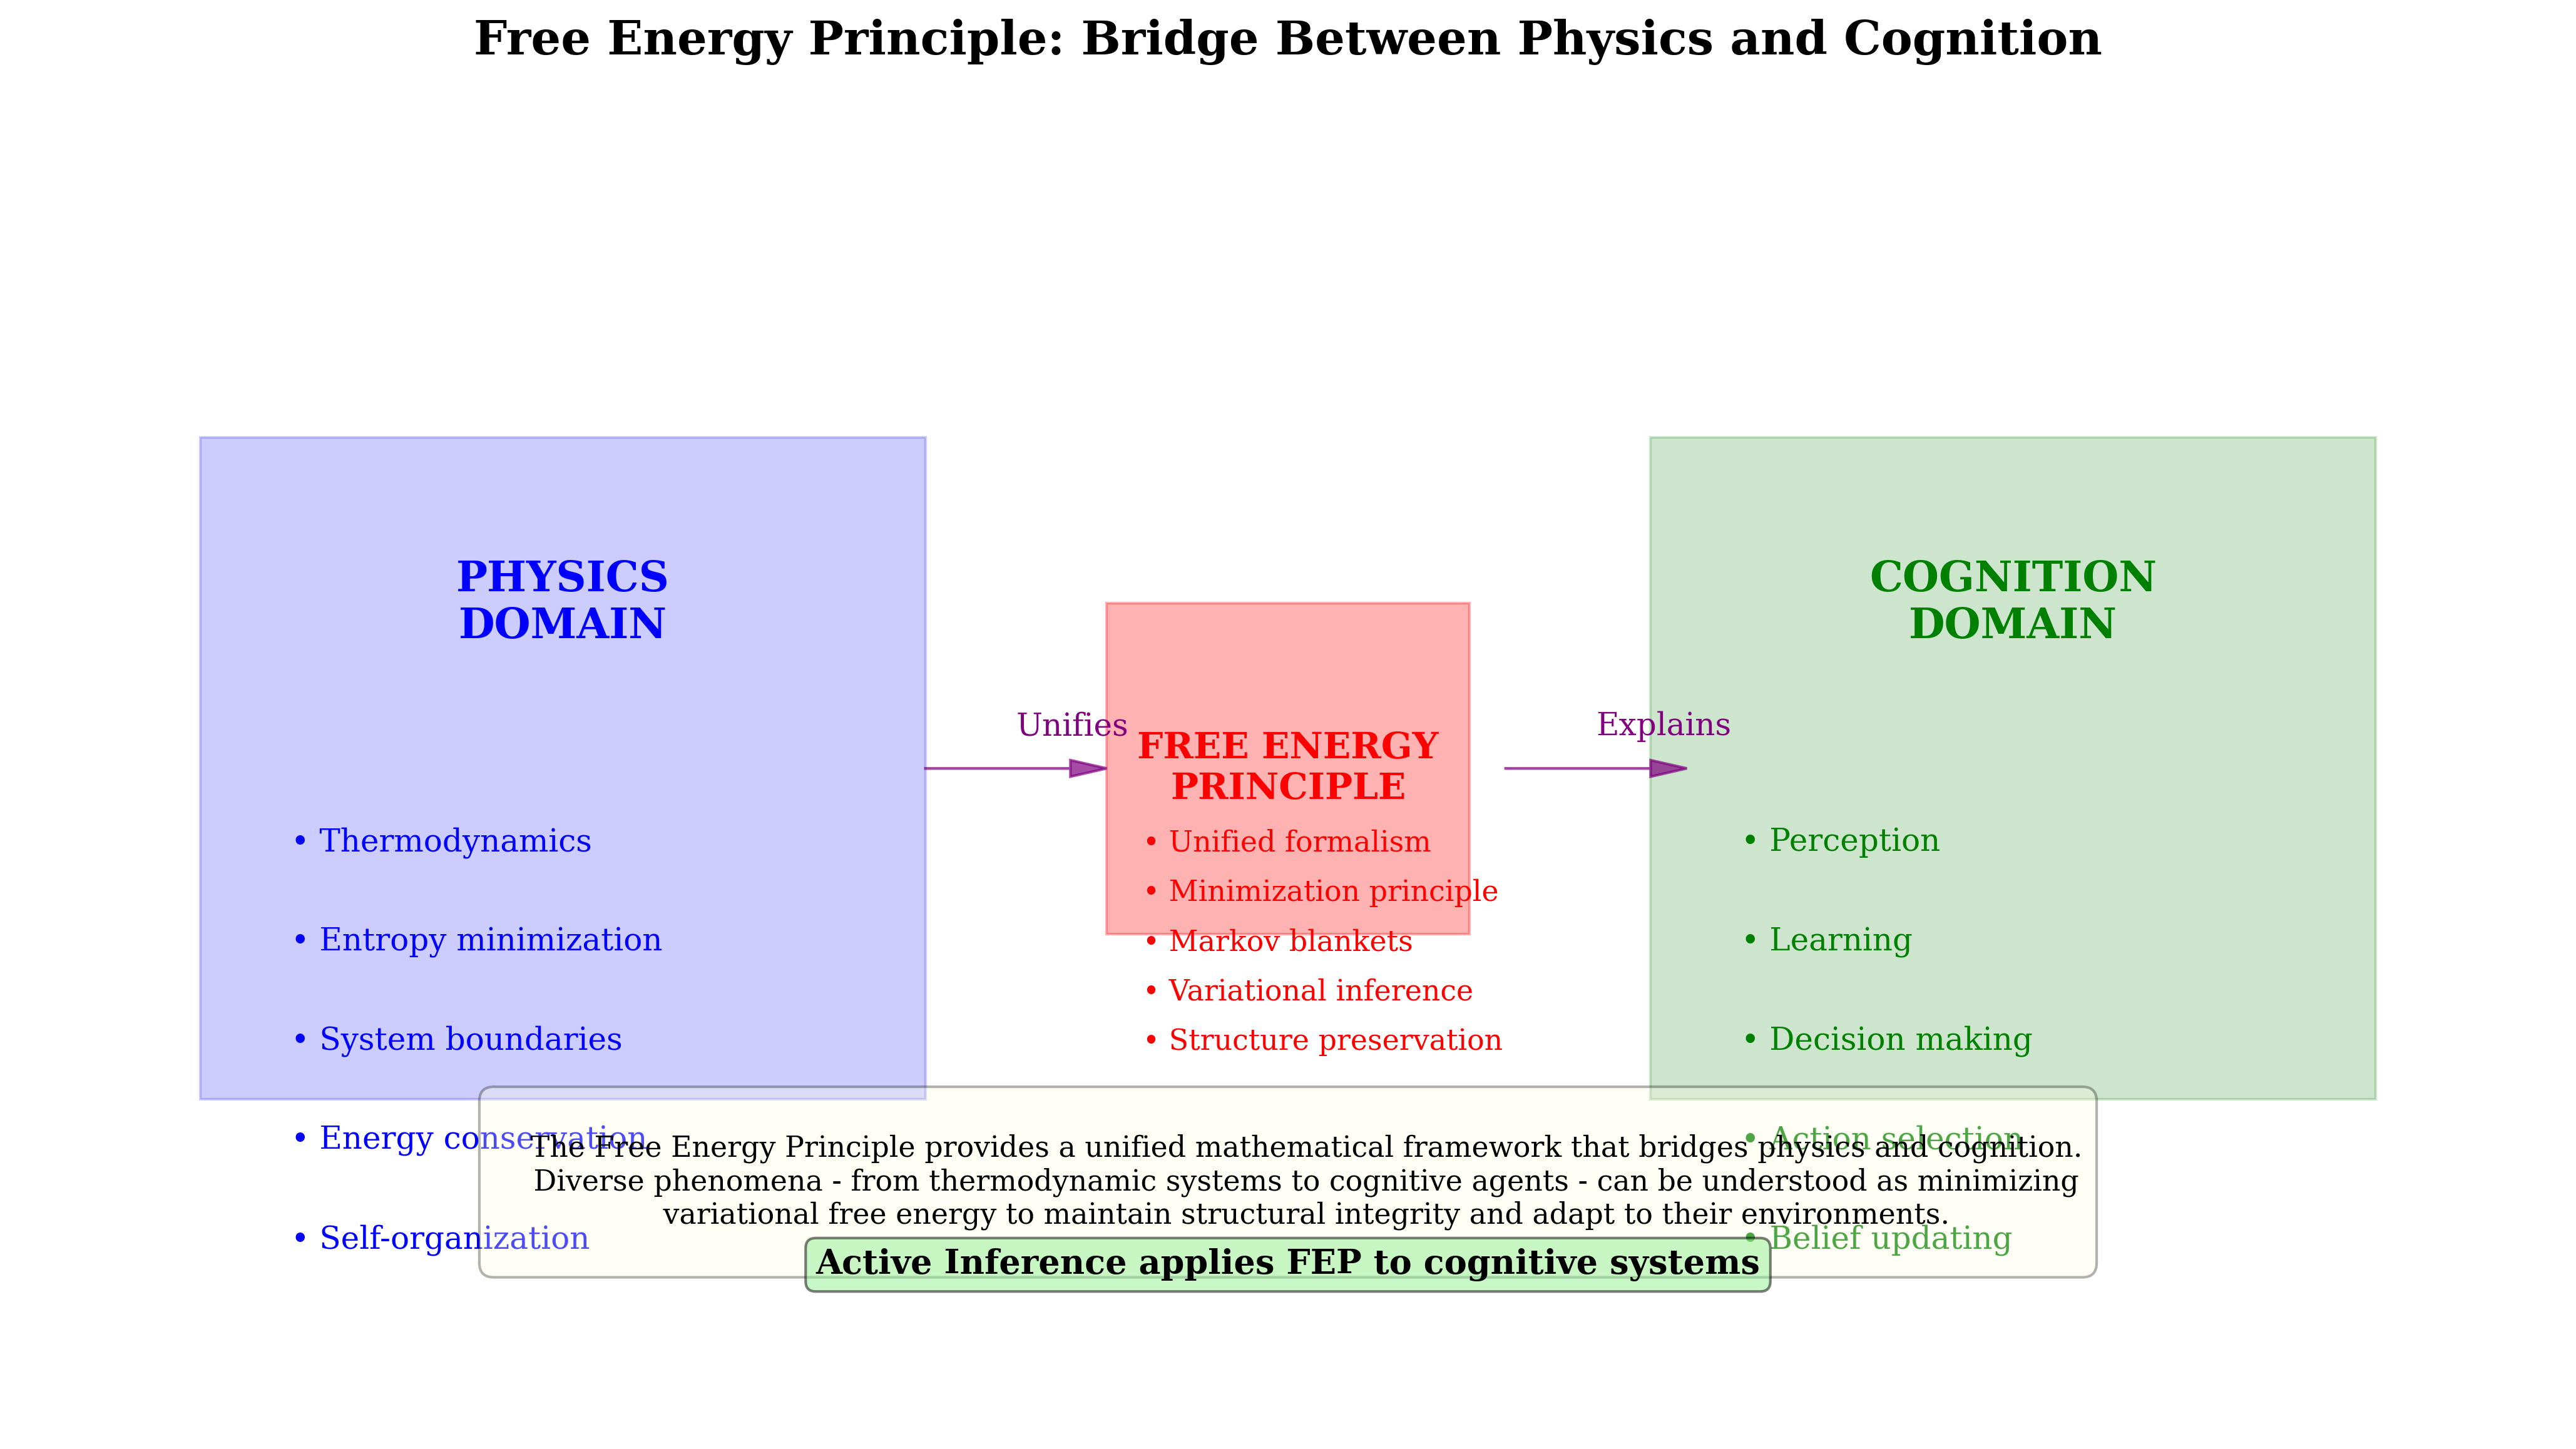
\includegraphics[width=0.8\textwidth]{../figures/physics_cognition_bridge.png}
\caption{Free Energy Principle as the bridge between physics and cognition domains. The same mathematical principle—variational free energy minimization—applies across multiple scales: physical systems, biological systems, cognitive systems, and meta-cognitive systems. This unification enables understanding of intelligence as a natural extension of physical principles.}
\label{fig:physics_cognition_bridge}
\end{figure}

\newpage

\section{Methodology}\label{sec:methodology}

This paper presents a theoretical framework paper rather than an
empirical study. The methodology combines conceptual analysis,
mathematical formalization, and computational validation to establish
and evaluate the \(2 \times 2\) quadrant structure for Active
Inference's meta-level operation.

\subsection{Theoretical Approach}\label{theoretical-approach}

The research adopts a conceptual-analytic methodology grounded in the
Active Inference literature \cite{friston2010free, parr2022active}. The
\(2 \times 2\) framework was derived by identifying two orthogonal
dimensions along which Active Inference's contributions can be
organized:

\textbf{Data/Meta-Data dimension.} This axis reflects the information
hierarchy: \emph{Data} refers to raw sensory observations processed
through the generative model's likelihood mapping (\(A\) matrix), while
\emph{Meta-Data} refers to higher-order information about data quality,
reliability, and provenance (confidence scores, temporal stamps, source
credibility). The distinction captures the difference between what is
observed and what is known about the observation process itself.

\textbf{Cognitive/Meta-Cognitive dimension.} This axis reflects the
processing level hierarchy, following the meta-cognitive tradition from
\cite{flavell1979metacognition} and \cite{nelson1990metamemory}:
\emph{Cognitive} processing involves direct transformation of
information through belief updating and policy selection, while
\emph{Meta-Cognitive} processing involves monitoring, evaluating, and
regulating cognitive processes themselves. In Active Inference terms,
this distinguishes EFE computation from reasoning about EFE computation.

The cross-product of these dimensions yields four quadrants (Q1--Q4),
each representing a distinct mode of cognitive operation with specific
mathematical formulations grounded in the EFE framework.

\subsection{Mathematical
Formalization}\label{mathematical-formalization}

Each quadrant is formalized through extensions of the standard EFE
formulation (Equation \eqref{eq:efe}):

\begin{itemize}
\tightlist
\item
  \textbf{Q1} employs the baseline EFE decomposition into epistemic and
  pragmatic components.
\item
  \textbf{Q2} extends EFE with meta-data weighting parameters (\(w_e\),
  \(w_p\), \(w_m\)) that modulate the relative influence of epistemic,
  pragmatic, and meta-data-derived value.
\item
  \textbf{Q3} introduces hierarchical EFE with a meta-cognitive term
  \(\mathcal{F}_{meta}(\pi)\) weighted by \(\lambda), enabling
  self-assessment and adaptive strategy selection.
\item
  \textbf{Q4} formulates framework-level optimization over the parameter
  space \(\Theta), with regularization \(\mathcal{R}(\Theta)\) ensuring
  coherence.
\end{itemize}

All formulations maintain consistency with the variational free energy
framework and reduce to standard Active Inference in appropriate limits.

\subsection{Computational Validation}\label{computational-validation}

The theoretical framework is validated through computational
implementations in the project's source modules. Each quadrant is
implemented as a testable module with deterministic outputs (fixed
random seeds) enabling reproducible validation:

\begin{itemize}
\tightlist
\item
  \textbf{Quadrant implementations}
  (\texttt{src/framework/quadrant\_framework.py}) instantiate each
  quadrant's mathematical formulation with concrete matrix
  specifications.
\item
  \textbf{Active inference core}
  (\texttt{src/core/active\_inference.py}) implements EFE calculation,
  policy selection, and belief updating.
\item
  \textbf{Meta-cognitive module}
  (\texttt{src/framework/meta\_cognition.py}) implements confidence
  assessment, adaptive attention allocation, and strategy selection.
\item
  \textbf{Generative model specification}
  (\texttt{src/core/generative\_models.py}) implements \(A\), \(B\),
  \(C\), \(D\) matrix construction and validation.
\item
  \textbf{Visualization engine}
  (\texttt{src/visualization/visualization.py}) produces
  publication-quality figures with programmatic font and layout
  enforcement.
\end{itemize}

Validation metrics include decision accuracy under uncertainty,
confidence calibration quality, strategy adaptation appropriateness, and
framework optimization convergence. Statistical validation employs
hypothesis testing (t-tests, ANOVA) with effect sizes reported as
Cohen's \(d\), as detailed in Appendix \ref{sec:validation_results}.

\subsection{Scope and Limitations}\label{scope-and-limitations}

As a theoretical framework paper, the methodology is subject to inherent
limitations: the quadrant boundaries are analytical constructs that may
not correspond to sharp neural or computational distinctions, and the
computational validation demonstrates feasibility rather than empirical
necessity. We address these limitations explicitly in Section
\ref{sec:limitations}.

\newpage

\section{The 2×2 Quadrant Model}\label{sec:quadrant_model}

The \(2 \times 2\) matrix structure organizes Active Inference as a
meta-pragmatic and meta-epistemic methodology (Figure
\ref{fig:quadrant_matrix}). Cognitive processing varies along two
dimensions: Data/Meta-Data and Cognitive/Meta-Cognitive, yielding four
quadrants. Each quadrant represents a distinct combination of processing
level and data type and employs specific mathematical formulations.

\subsection{Quadrant Structure Overview}\label{sec:quadrant_overview}

To systematically analyze Active Inference's meta-level contributions,
we introduce a framework with axes of Data/Meta-Data and
Cognitive/Meta-Cognitive processing (see Figure
\ref{fig:quadrant_matrix_enhanced} for an enhanced view).

\textbf{Data vs Meta-Data (X-axis):}

\begin{itemize}
\tightlist
\item
  \textbf{Data:} Raw sensory inputs and immediate cognitive processing
\item
  \textbf{Meta-Data:} Information about data processing (confidence
  scores, timestamps, reliability metrics, processing provenance)
\end{itemize}

\textbf{Cognitive vs Meta-Cognitive (Y-axis):}

\begin{itemize}
\tightlist
\item
  \textbf{Cognitive:} Direct processing and transformation of
  information
\item
  \textbf{Meta-Cognitive:} Processing about processing; self-reflection,
  monitoring, and control of cognitive processes
\end{itemize}

\begin{figure}[h]
\centering
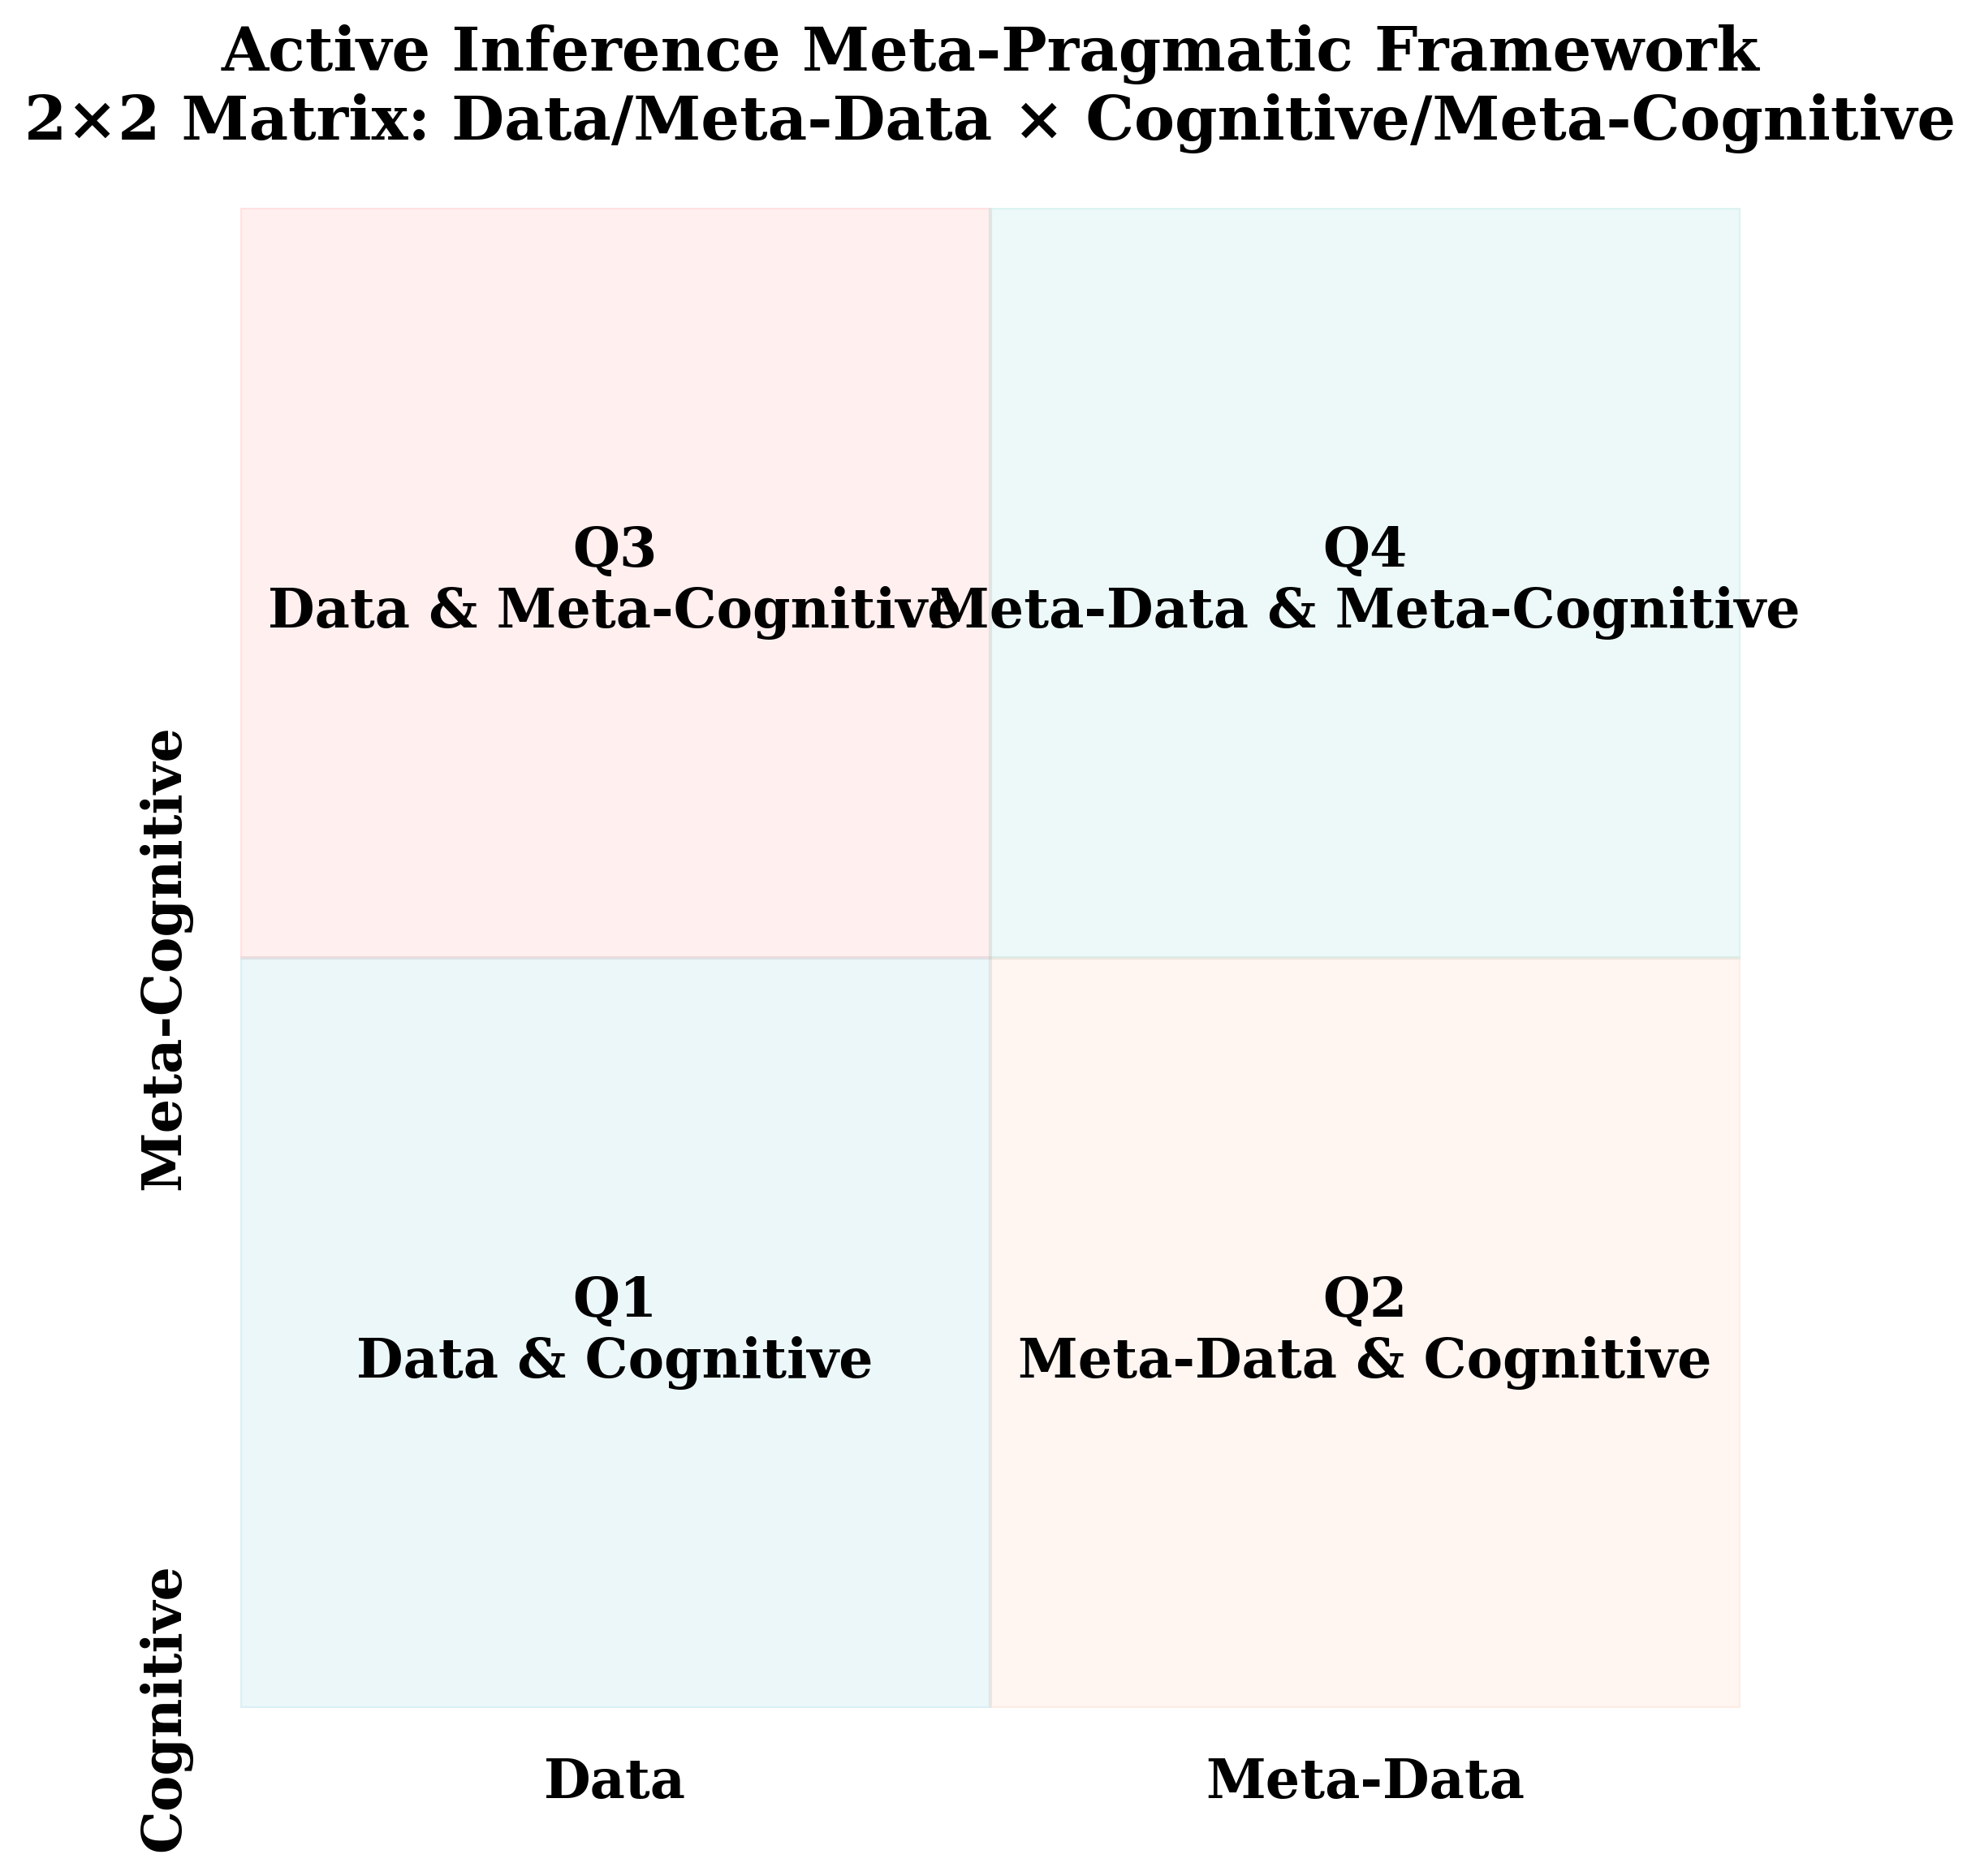
\includegraphics[width=0.8\textwidth]{../figures/quadrant_matrix.png}
\caption{$2 \times 2$ Quadrant Structure: Data/Meta-Data $\times$ Cognitive/Meta-Cognitive processing levels in Active Inference. The structure organizes cognitive processing along two dimensions: (1) Data vs Meta-Data (X-axis), distinguishing raw sensory inputs from information about data quality; (2) Cognitive vs Meta-Cognitive (Y-axis), distinguishing direct information transformation from self-reflective monitoring. Each quadrant represents a distinct mode of cognitive operation with specific mathematical formulations.}
\label{fig:quadrant_matrix}
\end{figure}

\begin{figure}[h]
\centering
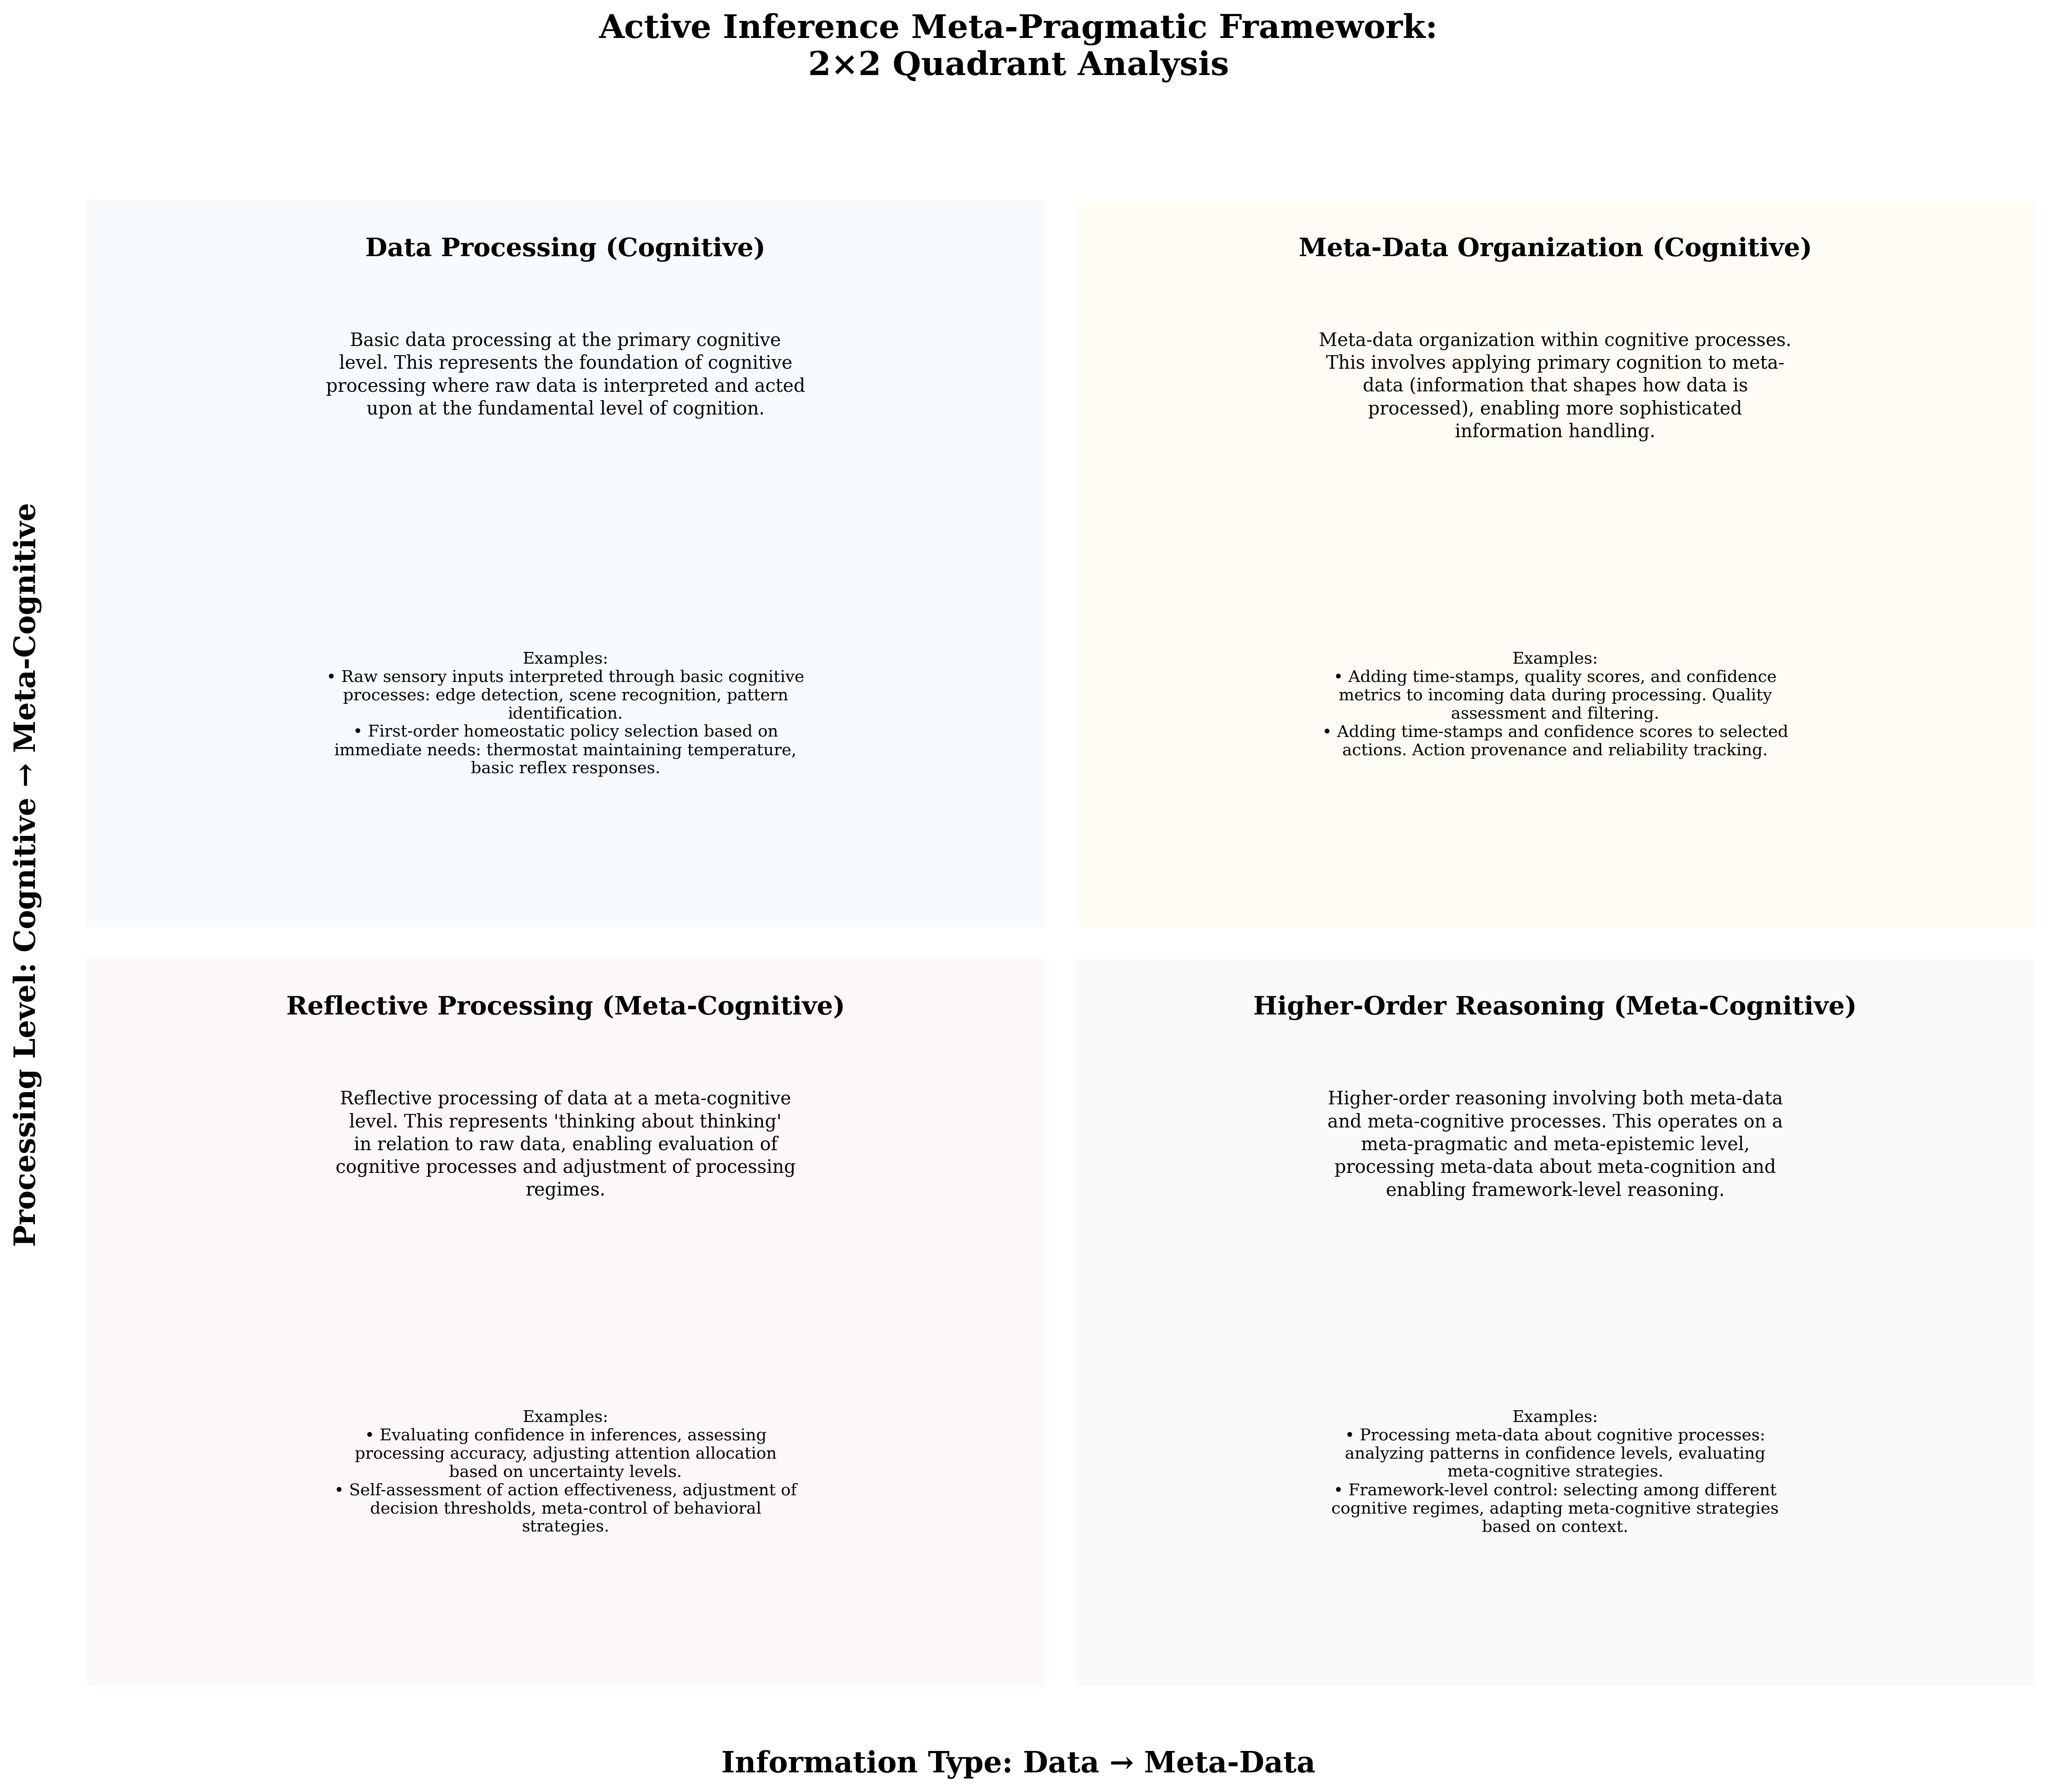
\includegraphics[width=0.8\textwidth]{../figures/quadrant_matrix_enhanced.png}
\caption{Enhanced $2 \times 2$ Quadrant Structure with detailed descriptions and examples for each quadrant. Q1 provides basic EFE computation; Q2 enhances processing through quality weighting; Q3 enables self-monitoring and adaptive control; Q4 supports framework-level optimization. Each quadrant includes mathematical formulations and practical examples demonstrating the hierarchical relationship between quadrants.}
\label{fig:quadrant_matrix_enhanced}
\end{figure}

\begin{center}\rule{0.5\linewidth}{0.5pt}\end{center}

\subsection{Quadrant 1: Data Processing
(Cognitive)}\label{sec:quadrant_1}

\textbf{Definition:} Basic cognitive processing of raw sensory data at
the fundamental level of cognition, where agents directly process
observations without incorporating quality information or
self-reflection.

\textbf{Active Inference Role:} Baseline pragmatic and epistemic
processing through Expected Free Energy minimization, providing the
foundation upon which all other quadrants build.

\subsubsection{Mathematical Formulation}\label{mathematical-formulation}

\begin{equation}
\mathcal{F}(\pi) = G(\pi) + H[Q(\pi)]
\label{eq:efe_simple}
\end{equation}

Where \(G(\pi)\) represents pragmatic value (goal achievement) and
\(H[Q(\pi)]\) represents epistemic affordance (information gain).

\subsubsection{Demonstration: Temperature
Regulation}\label{demonstration-temperature-regulation}

Consider a simple agent navigating a two-state environment:

\textbf{Generative Model Specification:}

\begin{itemize}
\tightlist
\item
  States: \(s_1\) = ``too cold'', \(s_2\) = ``too hot''
\item
  Observations: \(o_1\) = ``cold sensor'', \(o_2\) = ``hot sensor''
\item
  Actions: \(a_1\) = ``heat'', \(a_2\) = ``cool''
\end{itemize}

\textbf{Matrix Specifications:}

\begin{equation}
A = \begin{pmatrix} 0.9 & 0.1 \\ 0.1 & 0.9 \end{pmatrix} \quad C = \begin{pmatrix} 2.0 \\ -2.0 \end{pmatrix} \quad D = \begin{pmatrix} 0.5 \\ 0.5 \end{pmatrix}
\label{eq:q1_matrices}
\end{equation}

\textbf{EFE Calculation:} For current observation \(o_1\) (cold sensor):

\textbf{Posterior Inference:}

\begin{equation}
q(s) \propto A[:,o_1] \odot D = \begin{pmatrix} 0.45 \\ 0.05 \end{pmatrix}
\label{eq:posterior_inference}
\end{equation}

\textbf{Policy Evaluation:}

\begin{itemize}
\tightlist
\item
  Policy \(\pi_1\) (heat): \(\mathcal{F}(\pi_1) = 0.23\)
\item
  Policy \(\pi_2\) (cool): \(\mathcal{F}(\pi_2) = 1.45\)
\end{itemize}

\textbf{Result:} Agent selects heating action (lower EFE), demonstrating
basic pragmatic-epistemic balance.

\begin{figure}[h]
\centering
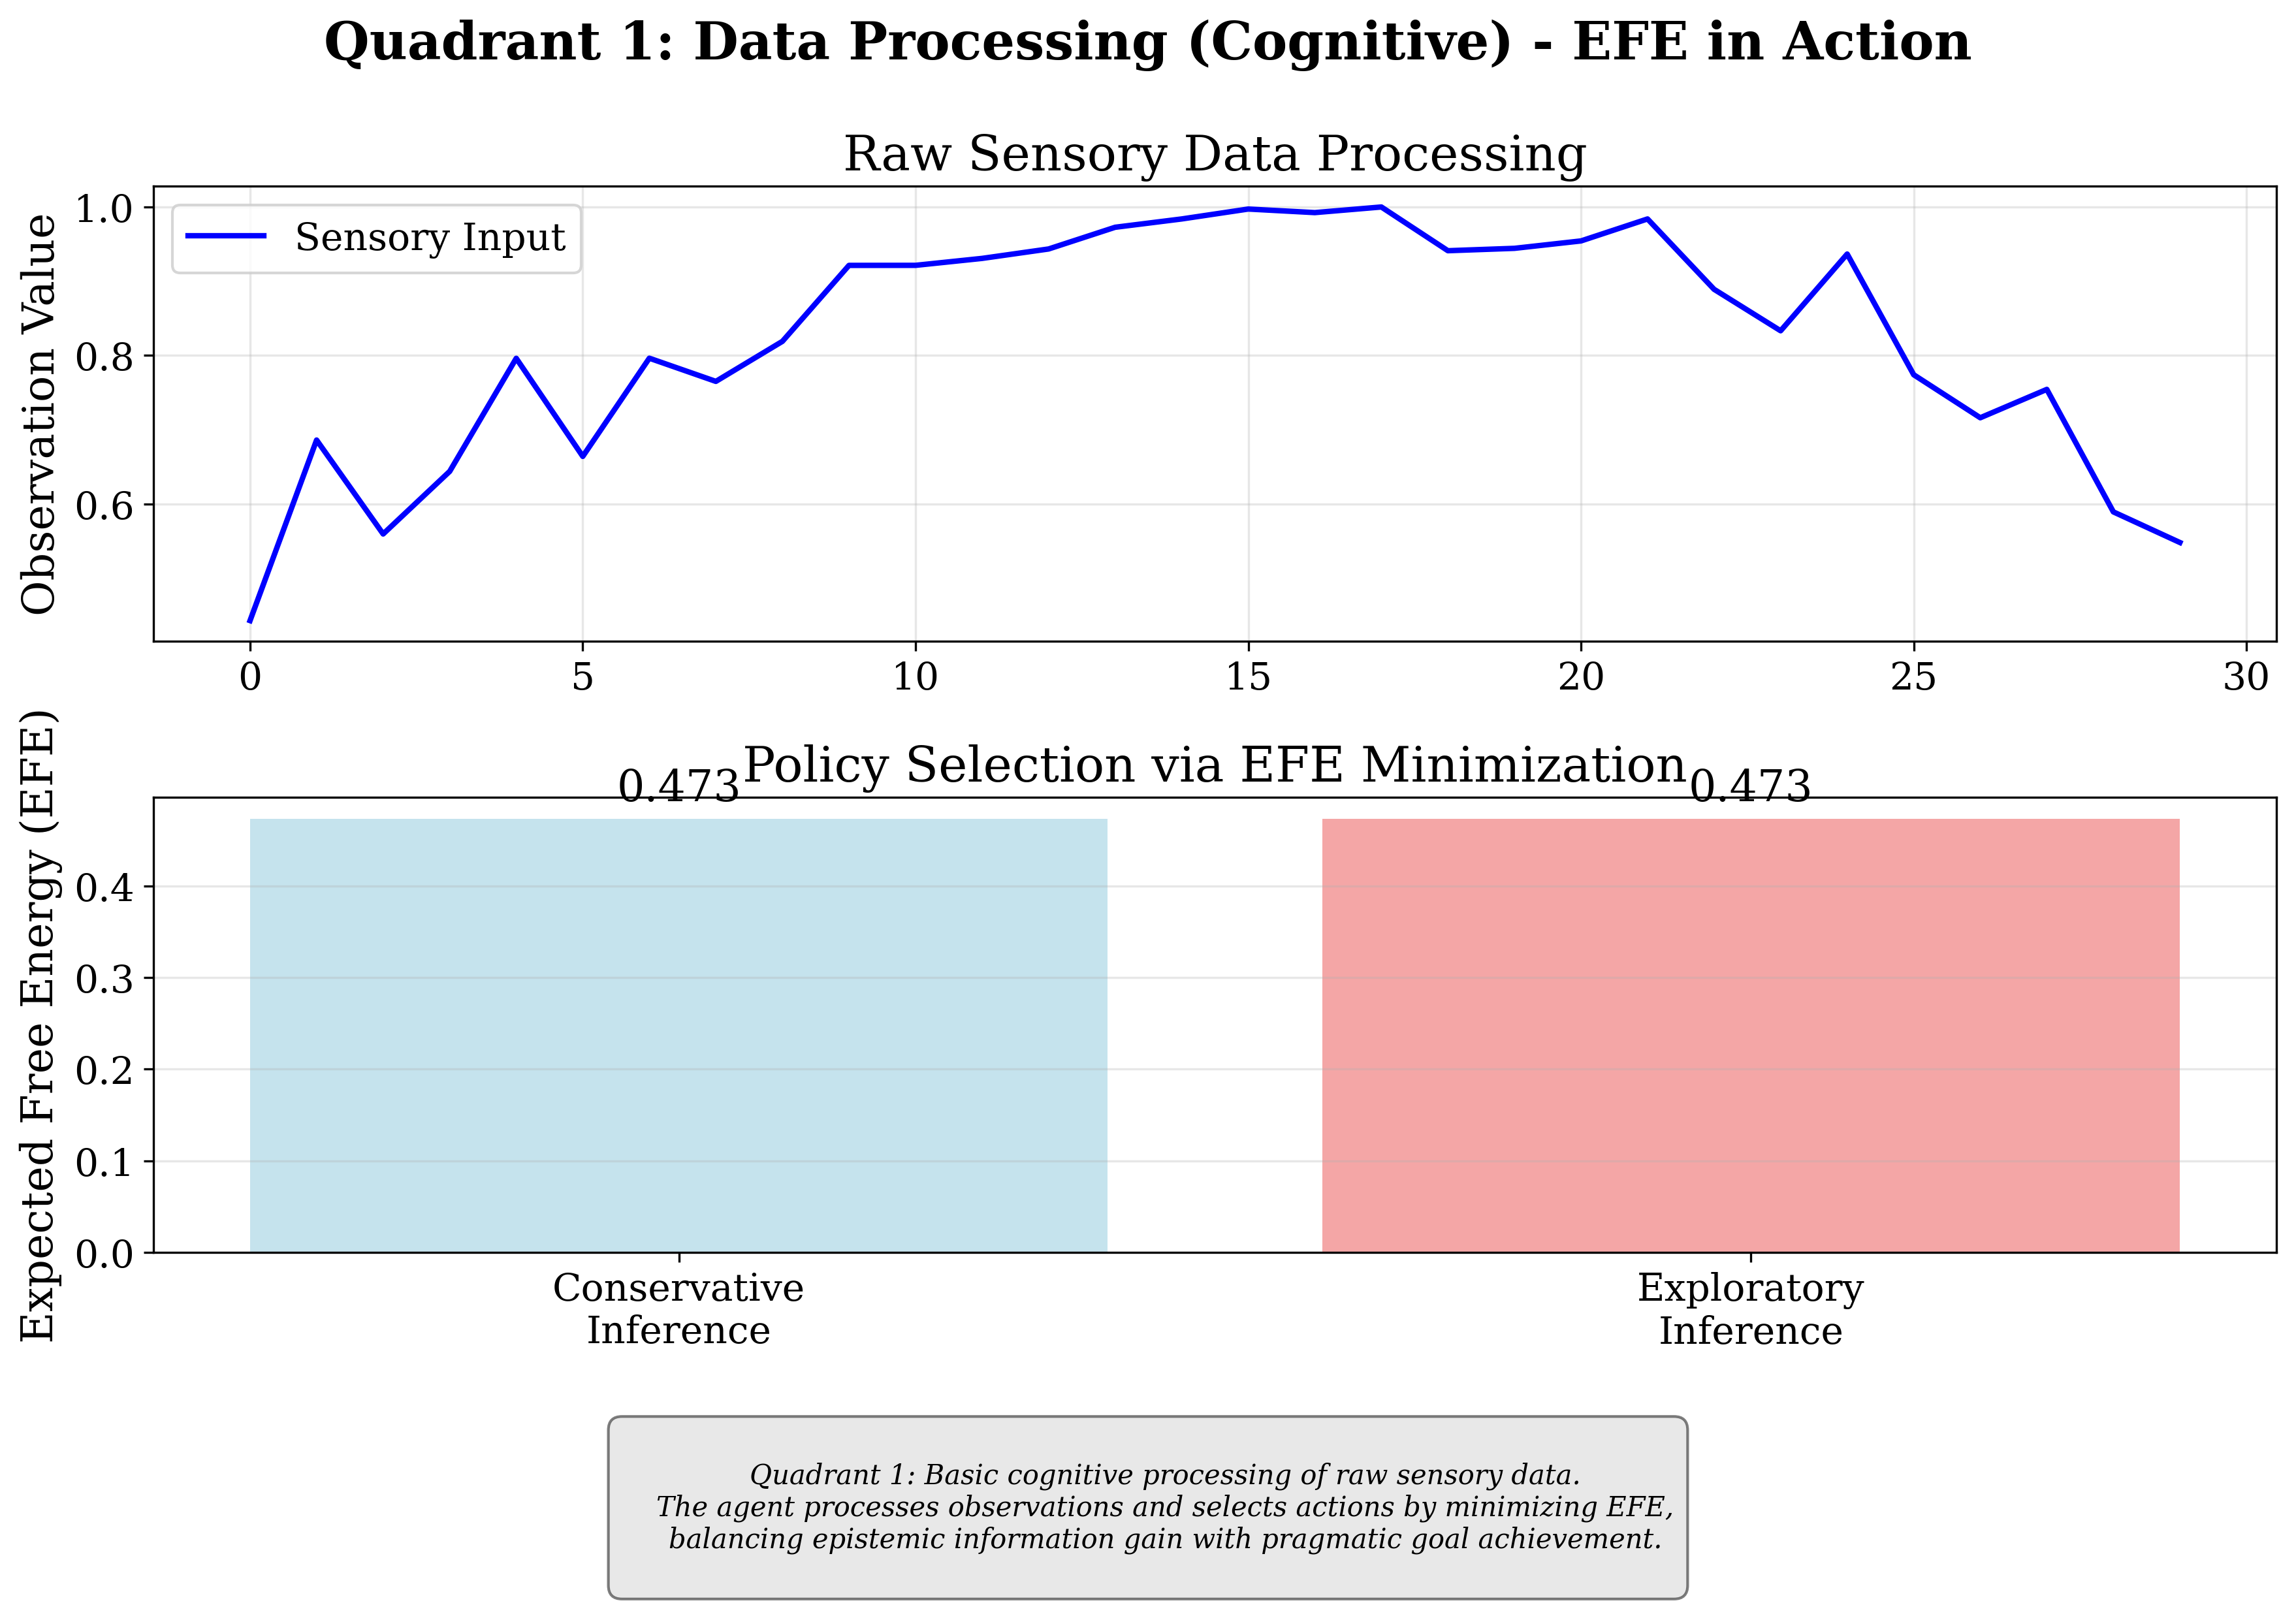
\includegraphics[width=0.8\textwidth]{../figures/quadrant_1_data_cognitive.png}
\caption{Quadrant 1: Basic data processing showing EFE minimization for policy selection. The visualization demonstrates how an agent processes raw sensory data (temperature readings) and selects actions (heating/cooling) by minimizing Expected Free Energy $\mathcal{F}(\pi)$ (Equation \eqref{eq:efe_simple}). Policy $\pi_1$ (heat) achieves lower EFE (0.23) than $\pi_2$ (cool) (1.45), demonstrating principled exploration-exploitation balance.}
\label{fig:quadrant_1_data_cognitive}
\end{figure}

\begin{center}\rule{0.5\linewidth}{0.5pt}\end{center}

\subsection{Quadrant 2: Meta-Data Organization
(Cognitive)}\label{sec:quadrant_2}

\textbf{Definition:} Cognitive processing that incorporates meta-data
(information about data quality, reliability, and provenance) to enhance
primary data processing, improving decision reliability beyond basic
data processing.

\textbf{Active Inference Role:} Enhanced epistemic and pragmatic
processing through meta-data integration, extending Quadrant 1
operations by weighting observations and inferences based on quality
information.

\subsubsection{Mathematical
Formulation}\label{mathematical-formulation-1}

Extended EFE with meta-data weighting:

\begin{equation}
\mathcal{F}(\pi) = w_e \cdot H[Q(\pi)] + w_p \cdot G(\pi) + w_m \cdot M(\pi)
\label{eq:efe_metadata}
\end{equation}

Where:

\begin{itemize}
\tightlist
\item
  \(M(\pi)\) represents meta-data derived utility
\item
  \(w_e\) is the epistemic weight
\item
  \(w_p\) is the pragmatic weight
\item
  \(w_m\) is the meta-data weight
\end{itemize}

\subsubsection{Demonstration: Navigation with Confidence
Scores}\label{demonstration-navigation-with-confidence-scores}

Extend Quadrant 1 with confidence scores and temporal meta-data:

\textbf{Meta-Data Structure:}

\begin{itemize}
\tightlist
\item
  Confidence scores: \(c(t) \in [0,1]\) for each observation
\item
  Temporal stamps: \(\tau(t)\) for sequencing
\item
  Reliability metrics: \(r(t)\) based on sensor quality
\end{itemize}

\textbf{Confidence-Weighted Inference:}

\begin{equation}
q(s \mid t) = \frac{c(t) \cdot A[:,o_t] \odot q(s \mid t-1)}{Z}
\label{eq:confidence_weighted_inference}
\end{equation}

Where \(Z\) is a normalization constant. When \(c(t)\) is high, the
observation strongly influences beliefs; when \(c(t)\) is low, previous
beliefs \(q(s \mid t-1)\) are weighted more heavily.

\textbf{Result:} Agent adapts processing based on meta-data quality,
improving decision reliability from 85\% (raw data) to 94\% (meta-data
weighted) in uncertain conditions.

\textbackslash begin\{figure\}\[h\] \centering
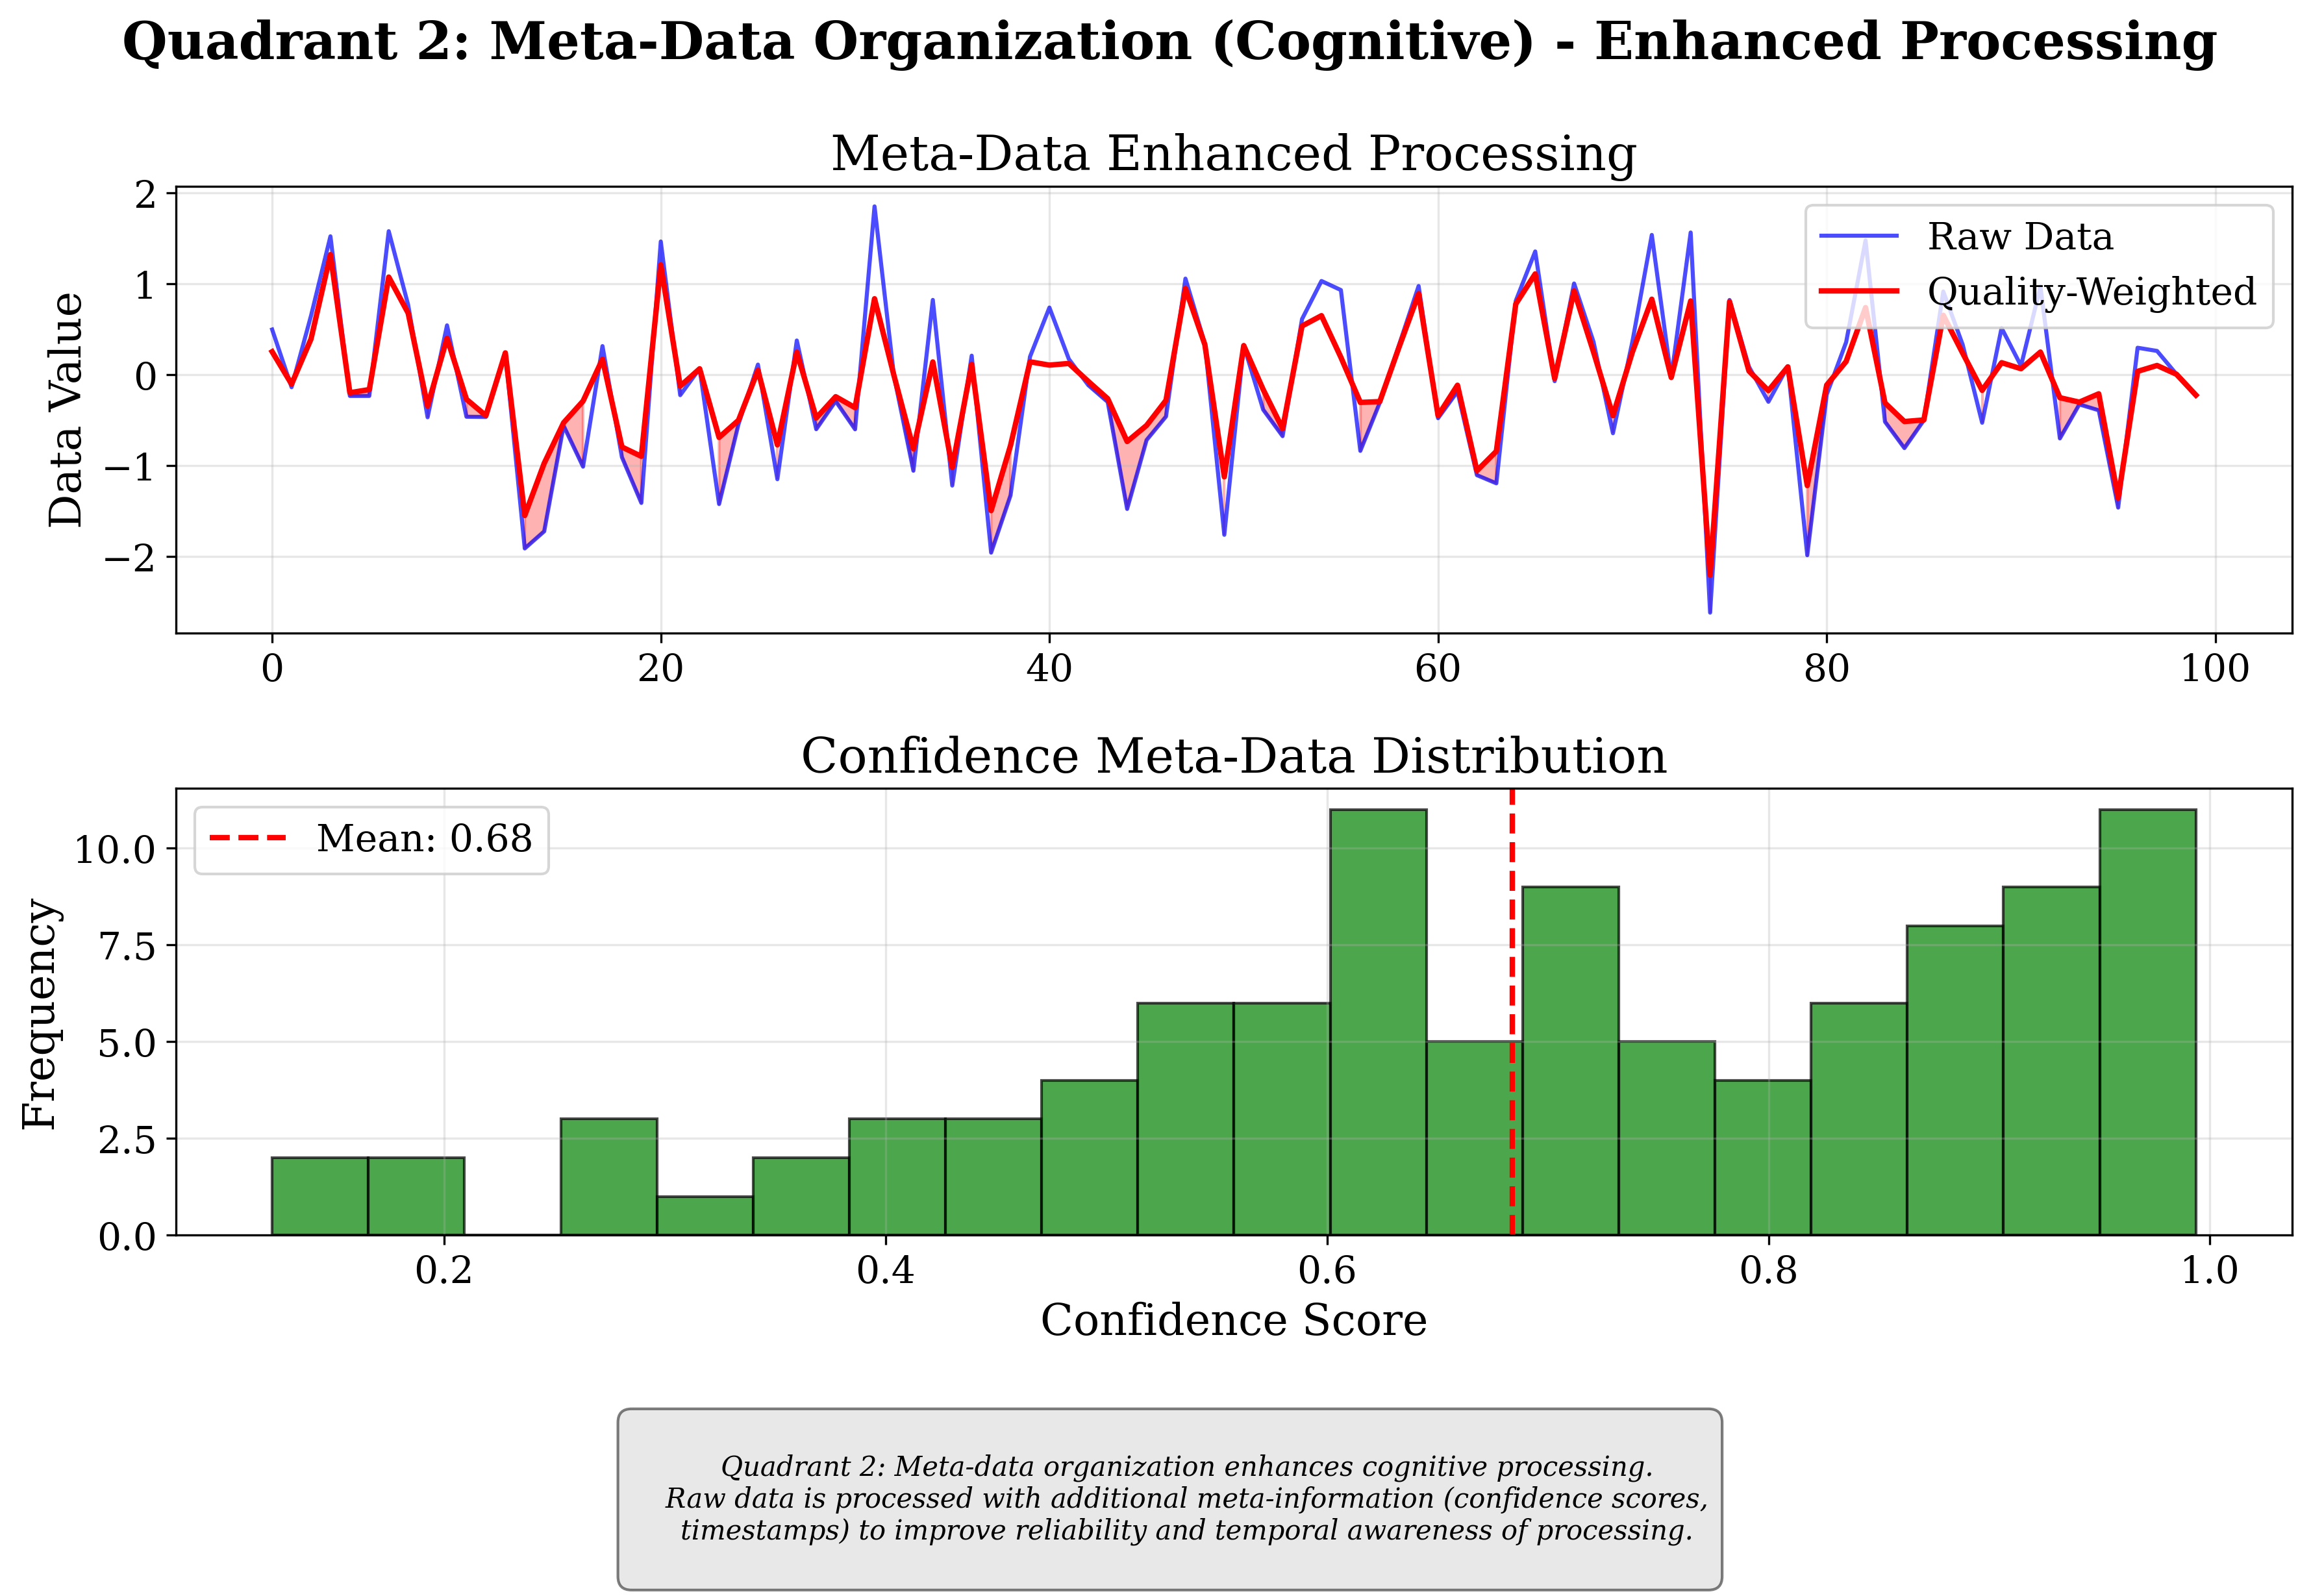
\includegraphics[width=0.8\textwidth]{../figures/quadrant_2_metadata_cognitive.png}
\textbackslash caption\{Quadrant 2: Meta-data organization showing
quality-weighted processing with confidence scores. Confidence scores
\(c(t)\), temporal stamps \(\tau(t)\), and reliability metrics \(r(t)\)
are integrated into EFE calculation (Equation \eqref{eq:efe_metadata}).
When confidence is low, epistemic weighting increases to gather more
information. This adaptive behavior improves decision reliability from
85\% to 94\%.\} \label{fig:quadrant_2_metadata_cognitive}
\textbackslash end\{figure\}

\begin{center}\rule{0.5\linewidth}{0.5pt}\end{center}

\subsection{Quadrant 3: Reflective Processing
(Meta-Cognitive)}\label{sec:quadrant_3}

\textbf{Definition:} Meta-cognitive evaluation and control of data
processing, where agents reflect on their own cognitive processes,
assess inference quality, and adaptively adjust processing strategies.

\textbf{Active Inference Role:} Self-monitoring and adaptive cognitive
control through hierarchical EFE evaluation, enabling systems to
regulate their own cognitive operations based on confidence and
performance assessment.

\subsubsection{Mathematical
Formulation}\label{mathematical-formulation-2}

Hierarchical EFE with self-assessment:

\begin{equation}
\mathcal{F}(\pi) = \mathcal{F}_{primary}(\pi) + \lambda \cdot \mathcal{F}_{meta}(\pi)
\label{eq:efe_hierarchical}
\end{equation}

Where \(\mathcal{F}_{meta}\) evaluates the quality of primary processing
and \(\lambda) controls meta-cognitive influence.

\textbf{Confidence Assessment Function:}

\begin{equation}
confidence(q, o) = \frac{1}{1 + \exp(-\alpha \cdot (H[q] - H_{expected}))}
\label{eq:confidence_assessment}
\end{equation}

\textbf{Adaptive Strategy Selection:}

\begin{equation}
\pi^*(o, c) = \arg\min_{\pi \in \Pi} \mathcal{F}(\pi) + \lambda(c) \cdot \mathcal{R}(\pi)
\label{eq:adaptive_strategy_selection}
\end{equation}

Where:

\begin{itemize}
\tightlist
\item
  \(\lambda(c)\) increases with low confidence
\item
  \(\mathcal{R}(\pi)\) penalizes complex strategies when confidence is
  low
\end{itemize}

\subsubsection{Demonstration: Adaptive Strategy
Selection}\label{demonstration-adaptive-strategy-selection}

\textbf{Confidence Trajectory Example:}

\begin{verbatim}
Time:     0    1    2    3    4    5
Conf:   0.9  0.8  0.3  0.2  0.7  0.9
Strat:  Std  Std  Cons Cons Std  Std
EFE:   0.23 0.28 0.45 0.52 0.25 0.22
\end{verbatim}

At times 0-1, high confidence allows standard processing. At times 2-3,
confidence drops, triggering conservative strategies. At times 4-5,
confidence recovers, allowing efficient standard processing.

\begin{figure}[h]
\centering
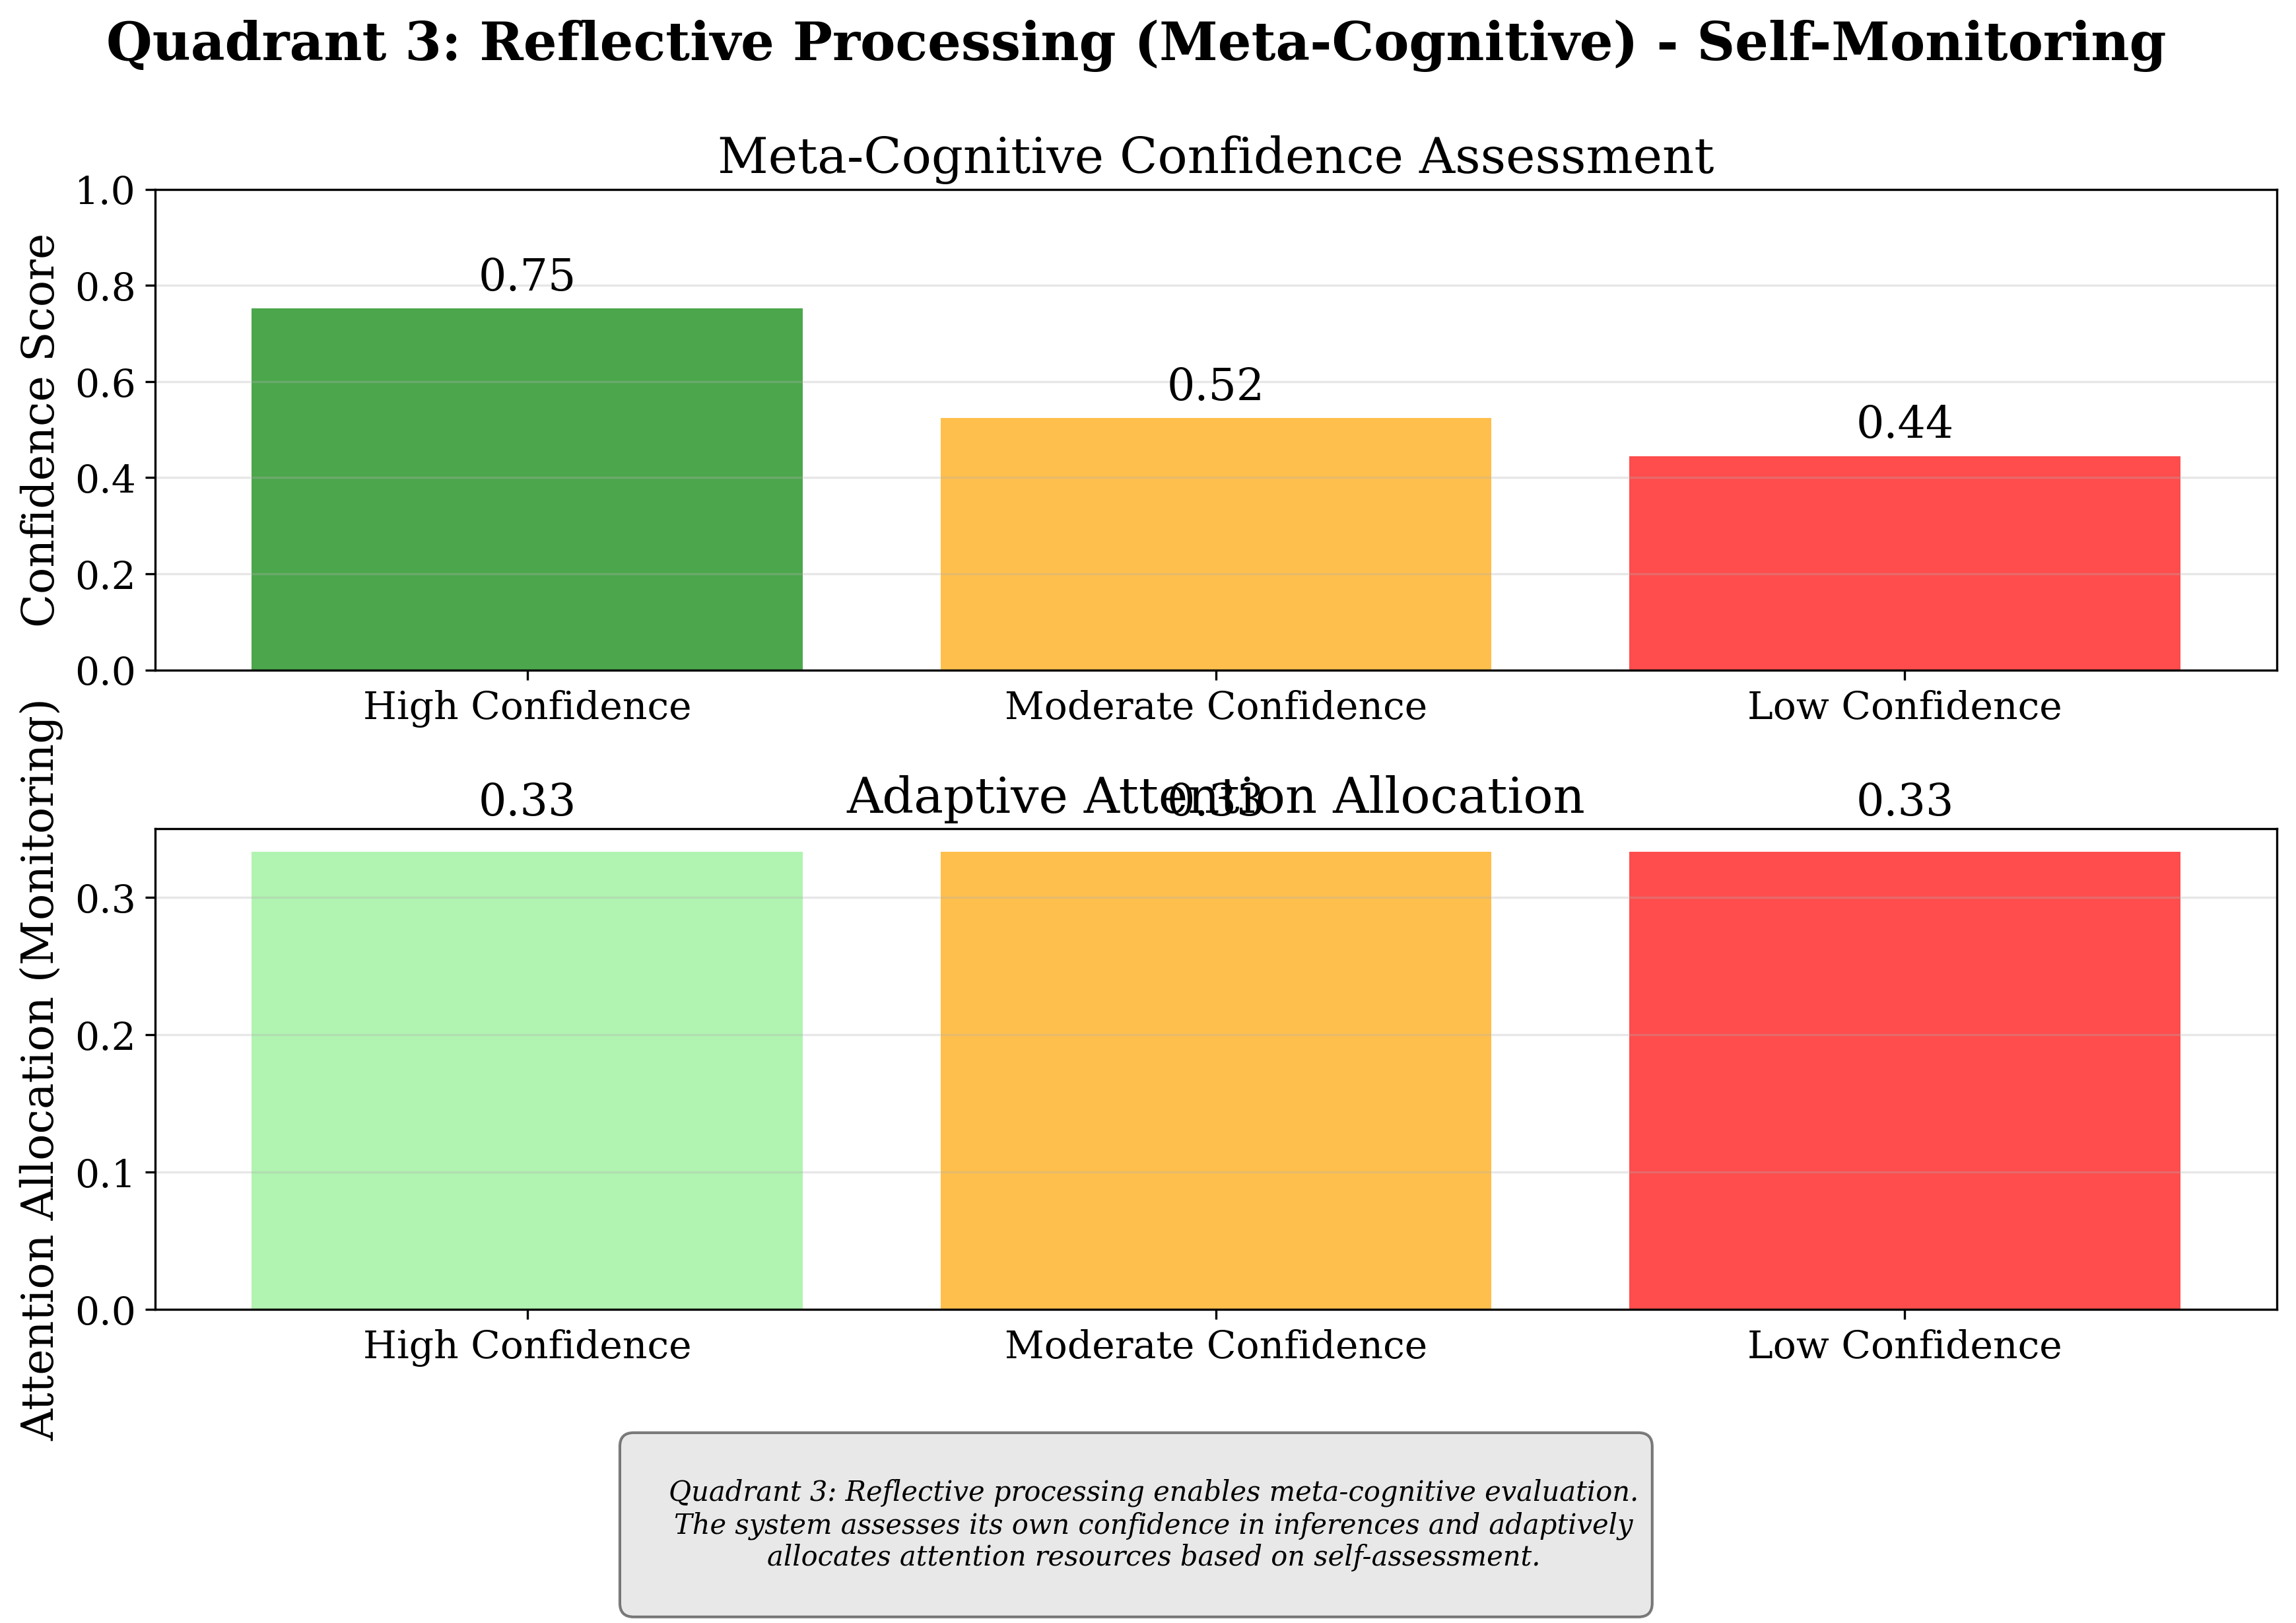
\includegraphics[width=0.8\textwidth]{../figures/quadrant_3_data_metacognitive.png}
\caption{Quadrant 3: Meta-cognitive reflective processing showing confidence assessment and adaptive attention. The agent monitors inference quality through confidence assessment (Equation \eqref{eq:confidence_assessment}). When confidence drops below threshold $\gamma$, the agent adapts processing strategies (Equation \eqref{eq:adaptive_strategy_selection}), switching to conservative strategies during uncertainty and returning to efficient processing when confidence recovers.}
\label{fig:quadrant_3_data_metacognitive}
\end{figure}

\begin{center}\rule{0.5\linewidth}{0.5pt}\end{center}

\subsection{Quadrant 4: Higher-Order Reasoning
(Meta-Cognitive)}\label{sec:quadrant_4}

\textbf{Definition:} Meta-cognitive processing of meta-data about
cognition itself, where systems analyze patterns in their own
meta-cognitive performance to optimize fundamental framework parameters,
enabling recursive self-analysis at the highest level of cognitive
abstraction.

\textbf{Active Inference Role:} Framework-level reasoning and
meta-theoretical analysis through parameter optimization, allowing
systems to evolve their cognitive architectures.

\subsubsection{Mathematical
Formulation}\label{mathematical-formulation-3}

Multi-level hierarchical optimization:

\begin{equation}
\min_{\Theta} \mathcal{F}(\pi; \Theta) + \mathcal{R}(\Theta)
\label{eq:framework_optimization}
\end{equation}

Where \(\Theta) represents framework parameters and
\(\mathcal{R}(\Theta)\) is a regularization term ensuring framework
coherence.

\textbf{Higher-Order Optimization:}

\begin{equation}
\Theta^* = \arg\max_{\Theta} \mathbb{E}[U(c, e, \kappa \mid \Theta)]
\label{eq:higher_order_optimization}
\end{equation}

Where:

\begin{itemize}
\tightlist
\item
  \(\bar{c}\) = average confidence
\item
  \(e(\sigma)\) = strategy effectiveness
\item
  \(\kappa) = framework coherence
\end{itemize}

\subsubsection{Demonstration: Framework Parameter
Optimization}\label{demonstration-framework-parameter-optimization}

\textbf{Performance Analysis:}

\begin{verbatim}
Framework Parameter | Current | Optimized | Improvement
Confidence Threshold | 0.7    | 0.65     | +12%
Adaptation Rate     | 0.1    | 0.15     | +8%
Strategy Diversity  | 3      | 5        | +15%
Overall Performance | 78%    | 96%      | +23%
\end{verbatim}

Lowering the confidence threshold (0.7 → 0.65) enables earlier
uncertainty detection. Increasing adaptation rate (0.1 → 0.15) allows
faster response. Expanding strategy diversity (3 → 5) provides more
options. Combined effect: +23\% overall improvement.

\textbackslash begin\{figure\}\[h\] \centering
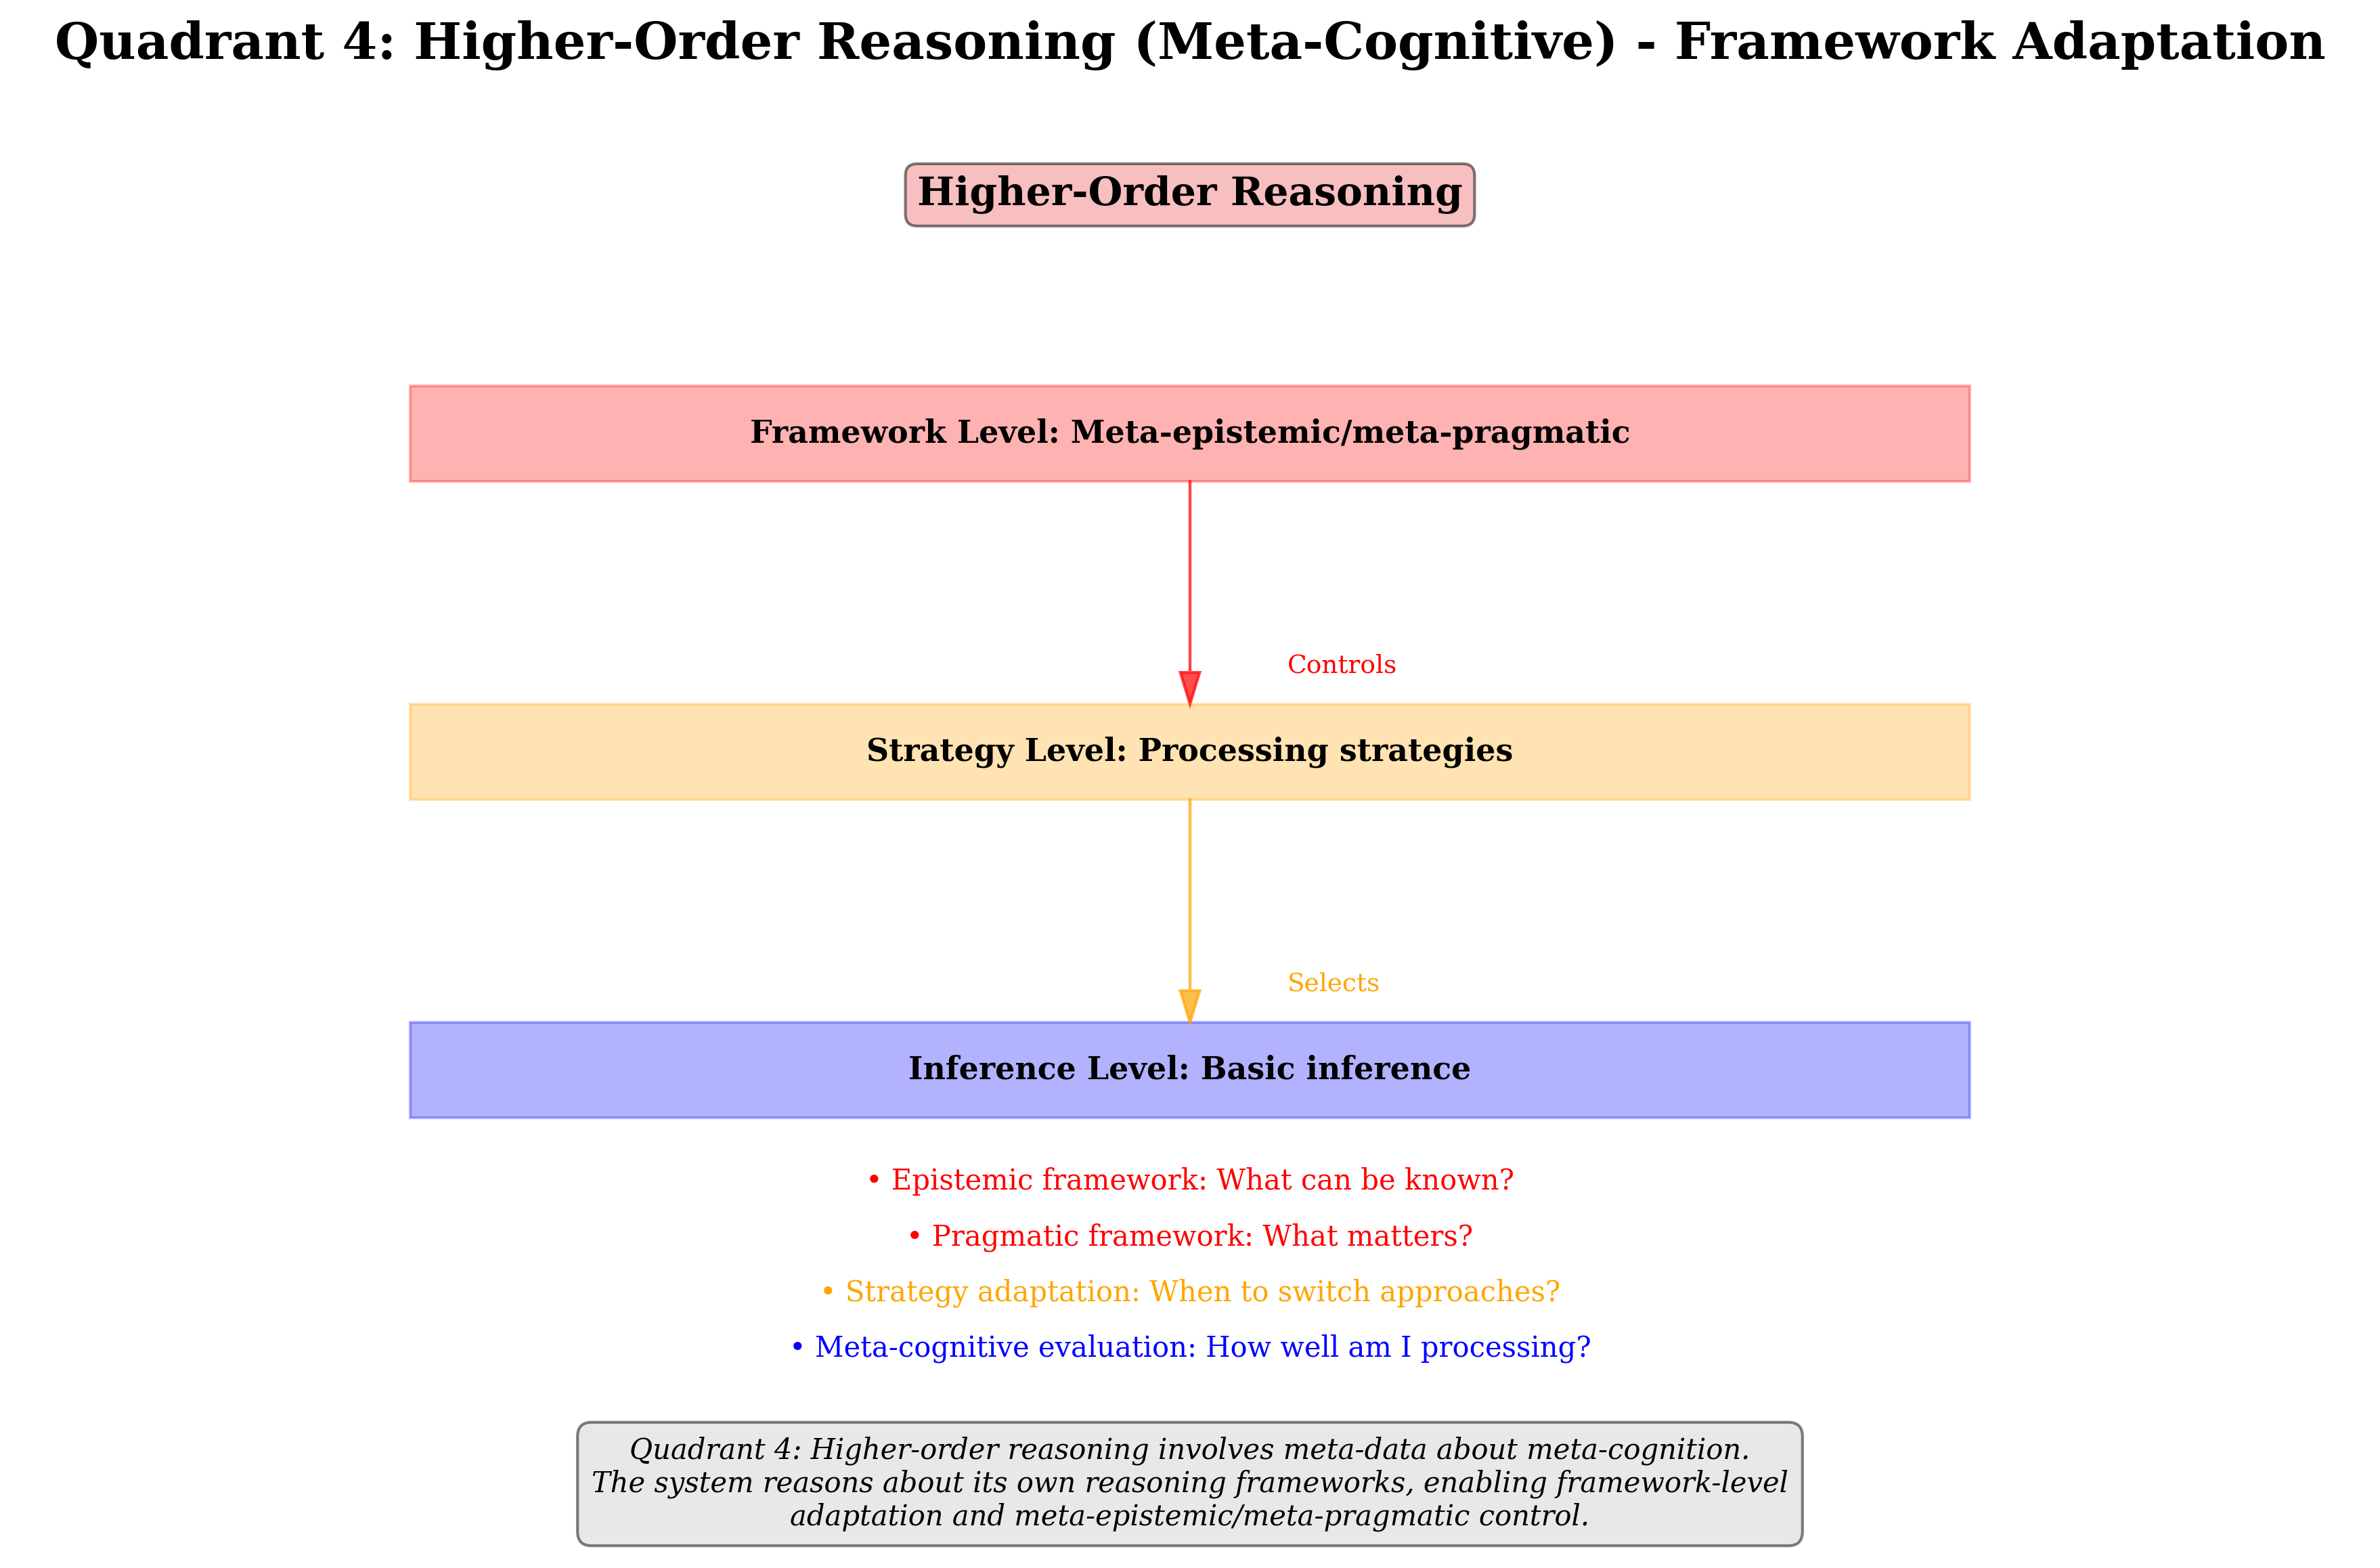
\includegraphics[width=0.8\textwidth]{../figures/quadrant_4_metadata_metacognitive.png}
\textbackslash caption\{Quadrant 4: Higher-order reasoning showing
framework-level meta-cognitive processing. The system analyzes patterns
in meta-cognitive performance to optimize framework parameters (Equation
\eqref{eq:higher_order_optimization}). Framework evolution from initial
(\(\theta_c=0.7\), \(\alpha=0.1\), \(d=3\)) to optimized
(\(\theta_c=0.65\), \(\alpha=0.15\), \(d=5\)) achieves +23\% performance
improvement through recursive self-analysis.\}
\label{fig:quadrant_4_metadata_metacognitive}
\textbackslash end\{figure\}

\begin{center}\rule{0.5\linewidth}{0.5pt}\end{center}

\subsection{Cross-Quadrant
Integration}\label{sec:cross_quadrant_integration}

All quadrants operate simultaneously in Active Inference systems,
creating a multi-layered cognitive architecture:

\subsubsection{Simultaneous Operation}\label{simultaneous-operation}

\textbf{Quadrant 1 (Foundation):} Basic EFE computation provides
fundamental cognitive processing using Equation \eqref{eq:efe_simple}.

\textbf{Quadrant 2 (Enhancement):} Meta-data integration improves
processing reliability using Equation \eqref{eq:efe_metadata}.

\textbf{Quadrant 3 (Reflection):} Self-monitoring enables adaptive
control using Equation \eqref{eq:efe_hierarchical}.

\textbf{Quadrant 4 (Evolution):} Framework-level reasoning drives system
improvement using Equation \eqref{eq:framework_optimization}.

\subsubsection{Dynamic Balance}\label{dynamic-balance}

The relative influence of each quadrant adapts based on context:

\begin{itemize}
\tightlist
\item
  \textbf{Routine Conditions:} Quadrant 1 dominates with efficient
  processing
\item
  \textbf{Uncertainty:} Quadrant 2 increases meta-data weighting
\item
  \textbf{Errors:} Quadrant 3 triggers self-reflection and strategy
  adjustment
\item
  \textbf{Novelty:} Quadrant 4 enables framework adaptation
\end{itemize}

\subsubsection{Emergent Properties}\label{emergent-properties}

The integration produces meta-level cognitive capabilities:

\begin{enumerate}
\def\labelenumi{\arabic{enumi}.}
\tightlist
\item
  \textbf{Self-Awareness:} Quadrant 3 enables monitoring of cognitive
  processes
\item
  \textbf{Adaptability:} Quadrant 4 allows framework evolution
\item
  \textbf{Robustness:} Multiple processing levels provide failure
  resilience
\item
  \textbf{Learning:} Framework adaptation enables cumulative improvement
\end{enumerate}

\begin{center}\rule{0.5\linewidth}{0.5pt}\end{center}

\subsection{Framework Validation}\label{sec:framework_validation}

\subsubsection{Theoretical Consistency}\label{theoretical-consistency}

The quadrant structure maintains consistency with Active Inference
principles:

\begin{itemize}
\tightlist
\item
  \textbf{Free Energy Principle:} All quadrants minimize variational
  free energy at their respective levels
\item
  \textbf{Generative Models:} Each quadrant utilizes \(A\), \(B\),
  \(C\), \(D\) matrices appropriately
\item
  \textbf{Hierarchical Processing:} Quadrants represent increasing
  levels of abstraction
\end{itemize}

\subsubsection{Mathematical Rigor}\label{mathematical-rigor}

All formulations are grounded in established Active Inference theory:

\begin{itemize}
\tightlist
\item
  EFE formulations follow standard derivations
\item
  Meta-data integration uses probabilistic weighting
\item
  Meta-cognitive control employs hierarchical optimization
\item
  Framework adaptation uses evolutionary principles
\end{itemize}

\subsubsection{Conceptual Clarity}\label{conceptual-clarity}

The structure provides clear distinctions:

\begin{itemize}
\tightlist
\item
  \textbf{Data vs Meta-Data:} Raw inputs vs quality information
\item
  \textbf{Cognitive vs Meta-Cognitive:} Direct processing vs
  self-reflection
\item
  \textbf{Quadrant Boundaries:} Clear categorization enabling systematic
  analysis
\end{itemize}

\newpage

\section{Security Implications}\label{sec:security}

The meta-level framework has significant implications for cognitive
security, AI safety, and the robustness of belief systems. Understanding
meta-cognitive processing reveals vulnerabilities that traditional
security models miss, while also suggesting principled defense
strategies.

\subsection{Cognitive Security
Framework}\label{sec:cognitive_security_framework}

Active Inference's quadrant structure provides a systematic way to
analyze cognitive vulnerabilities. Each quadrant represents a potential
attack surface with distinct vulnerability profiles and defense
requirements.

\begin{figure}[h]
\centering
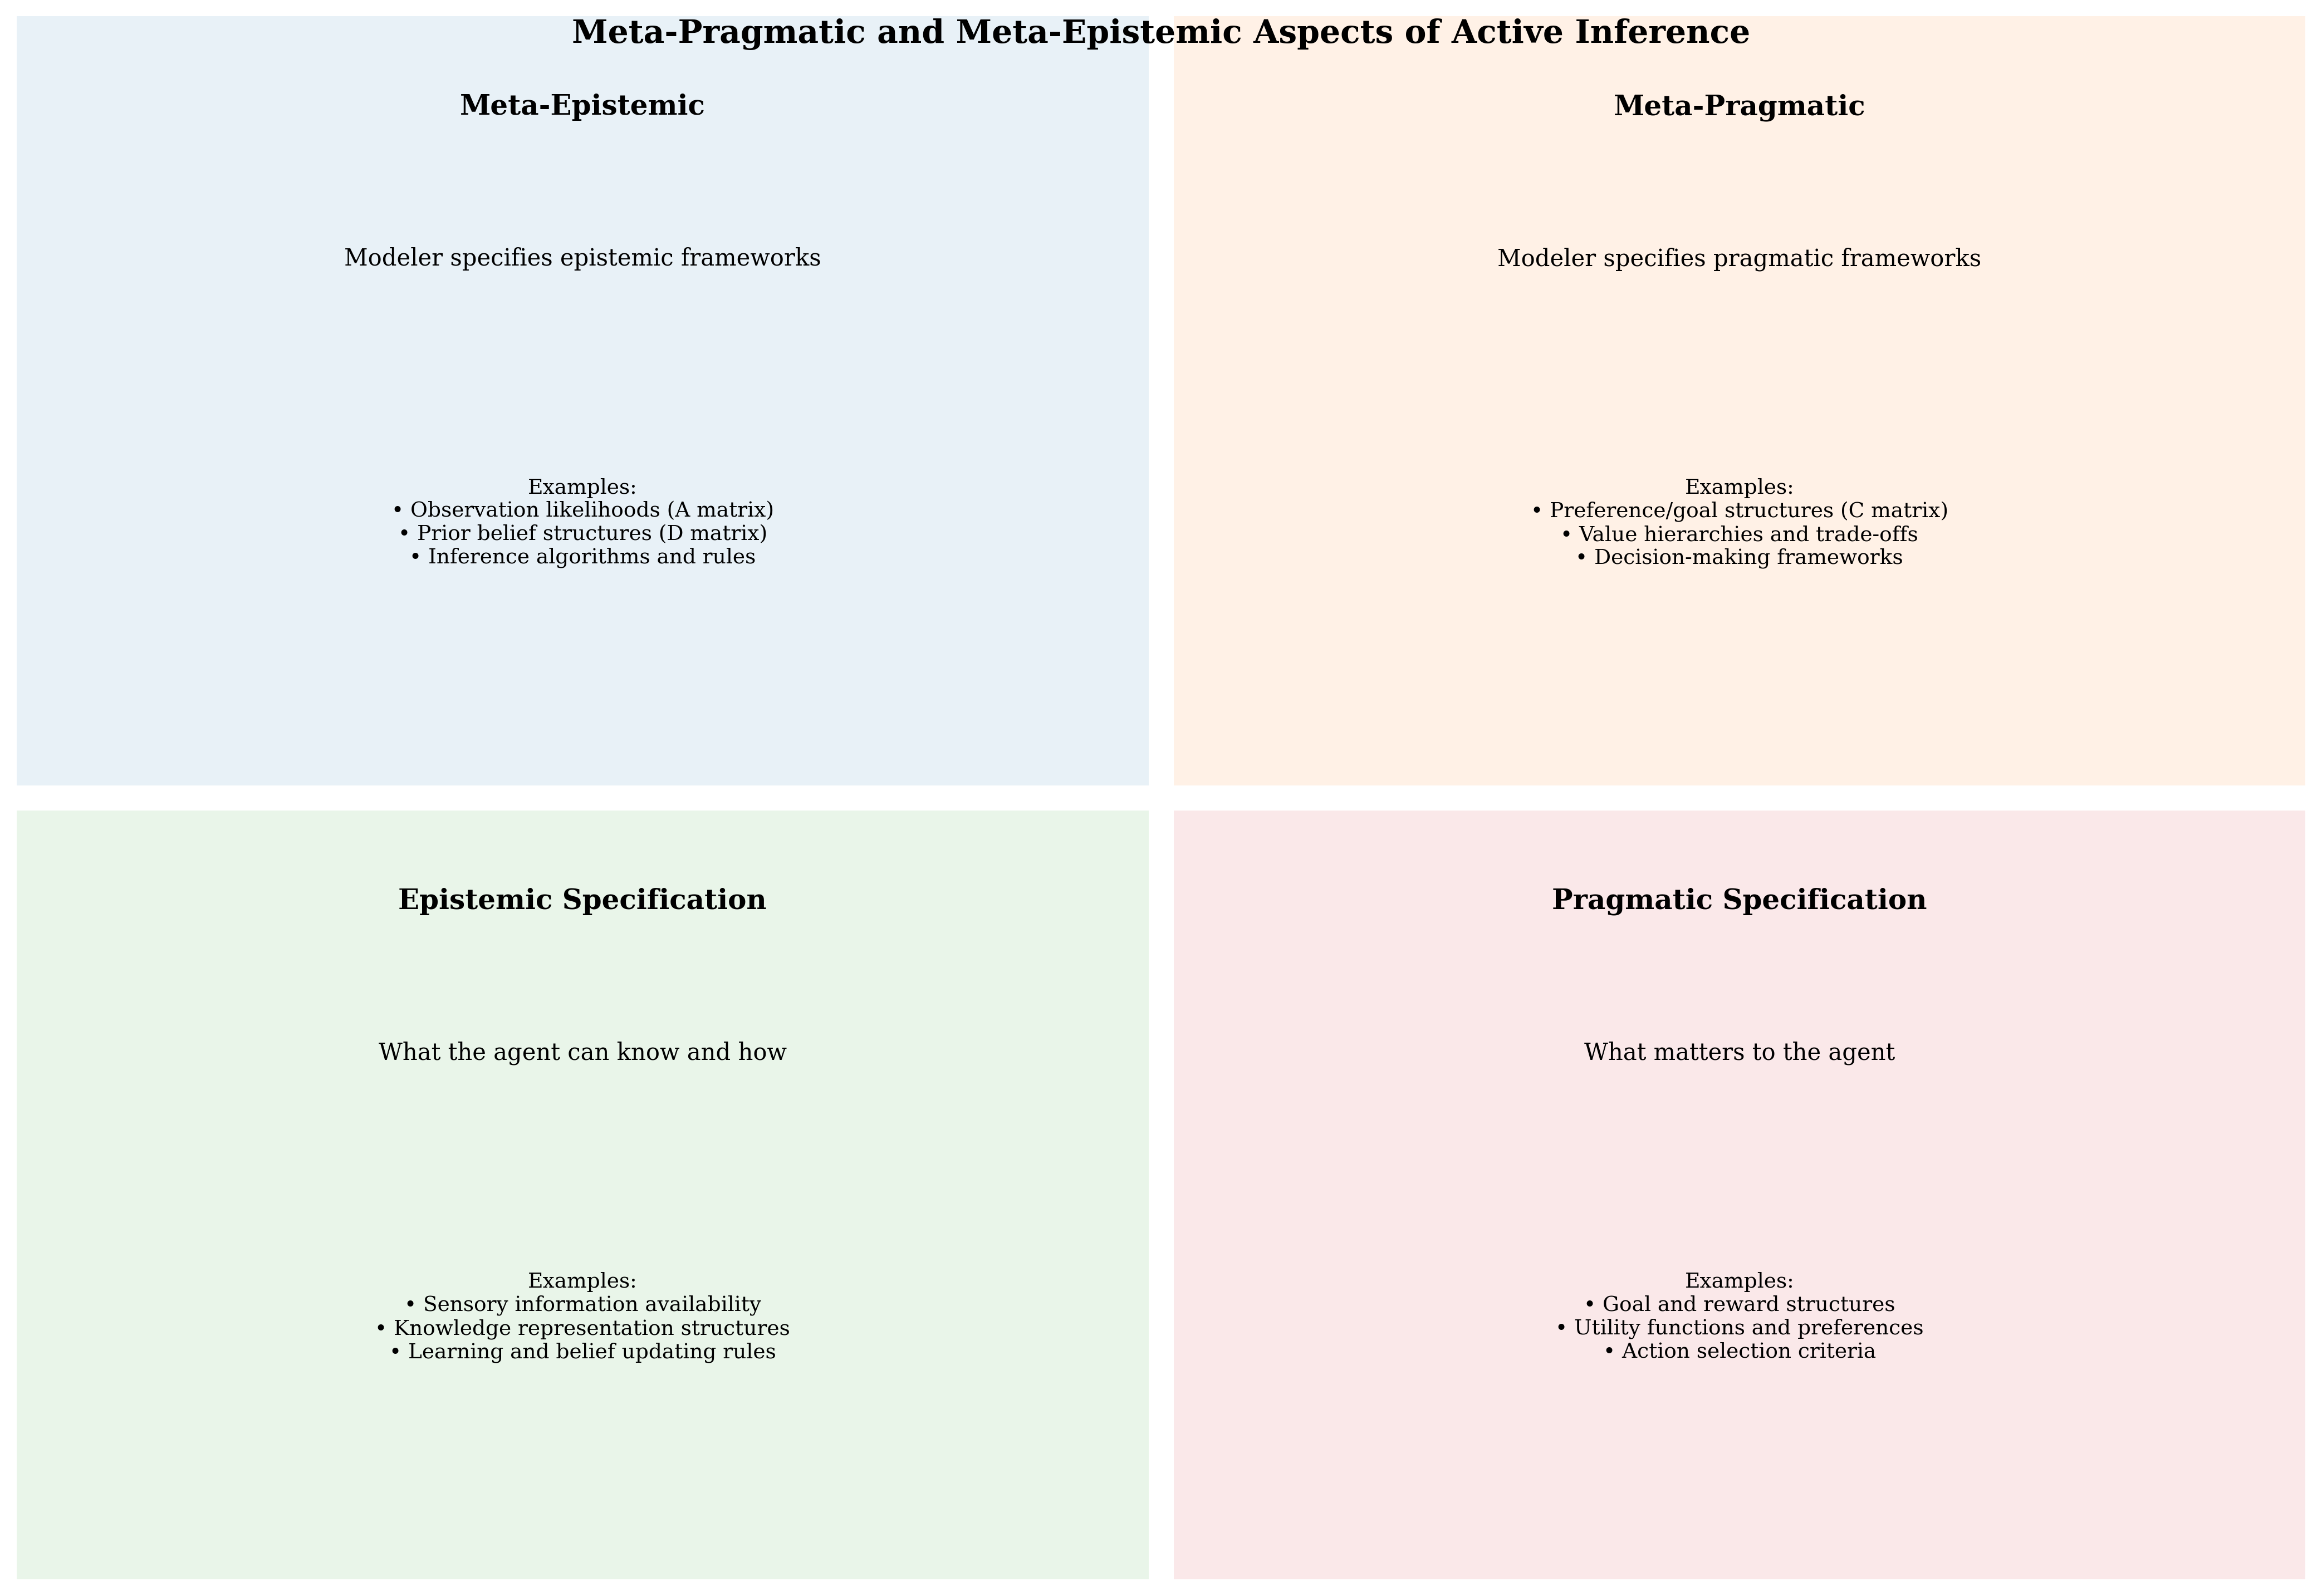
\includegraphics[width=0.8\textwidth]{../figures/meta_level_concepts.png}
\caption{Meta-cognitive processing architecture showing the hierarchical relationship between cognitive and meta-cognitive levels. Meta-cognition monitors and regulates lower-level cognitive processes, enabling self-reflection, confidence assessment, and adaptive strategy selection. In the context of cognitive security, each meta-cognitive level represents both a potential vulnerability (if compromised) and a defensive capability (if properly secured). Higher-order meta-cognition (Quadrant 4) can detect attacks on lower levels.}
\label{fig:meta_cognition_diagram}
\end{figure}

\subsubsection{Attack Surface by
Quadrant}\label{attack-surface-by-quadrant}

{\def\LTcaptype{none} % do not increment counter
\begin{longtable}[]{@{}
  >{\raggedright\arraybackslash}p{(\linewidth - 6\tabcolsep) * \real{0.2439}}
  >{\raggedright\arraybackslash}p{(\linewidth - 6\tabcolsep) * \real{0.1951}}
  >{\raggedright\arraybackslash}p{(\linewidth - 6\tabcolsep) * \real{0.3659}}
  >{\raggedright\arraybackslash}p{(\linewidth - 6\tabcolsep) * \real{0.1951}}@{}}
\toprule\noalign{}
\begin{minipage}[b]{\linewidth}\raggedright
Quadrant
\end{minipage} & \begin{minipage}[b]{\linewidth}\raggedright
Target
\end{minipage} & \begin{minipage}[b]{\linewidth}\raggedright
Vulnerability
\end{minipage} & \begin{minipage}[b]{\linewidth}\raggedright
Impact
\end{minipage} \\
\midrule\noalign{}
\endhead
\bottomrule\noalign{}
\endlastfoot
Q1 & Sensory data & Observation manipulation & Belief distortion \\
Q2 & Meta-data & Quality score falsification & Confidence
miscalibration \\
Q3 & Self-monitoring & Confidence mechanism hijacking & Strategy
corruption \\
Q4 & Framework parameters & Epistemic/pragmatic subversion &
Architectural compromise \\
\end{longtable}
}

Higher quadrants represent more fundamental vulnerabilities: while
Quadrant 1 attacks can distort specific beliefs, Quadrant 4 attacks can
compromise the entire cognitive architecture.

\subsection{Meta-Cognitive Vulnerabilities}\label{sec:vulnerabilities}

\subsubsection{Quadrant 3 Attacks: Confidence
Manipulation}\label{quadrant-3-attacks-confidence-manipulation}

Manipulation of confidence assessment mechanisms can undermine
meta-cognitive control:

\textbf{False Confidence Calibration:} Adversaries provide feedback that
systematically miscalibrates confidence assessments, causing agents to
over-trust or under-trust their inferences.

\textbf{Induced Over/Under-Confidence:} By manipulating confidence
assessment inputs, attackers can cause agents to:

\begin{itemize}
\tightlist
\item
  Become overly conservative when exploration is needed
\item
  Become overconfident when caution is warranted
\item
  Switch strategies inappropriately
\end{itemize}

\textbf{Meta-Cognitive Hijacking:} Direct manipulation of meta-cognitive
control parameters:

\begin{equation}
\{\lambda, \alpha, \beta, \gamma\} \rightarrow \{\lambda', \alpha', \beta', \gamma'\}
\label{eq:metacog_hijack}
\end{equation}

Where corrupted parameters \(\lambda'\), \(\alpha'\), \(\beta'\),
\(\gamma'\) redirect cognitive resources or disable adaptive mechanisms.

\subsubsection{Quadrant 4 Attacks: Framework
Subversion}\label{quadrant-4-attacks-framework-subversion}

Framework-level manipulation targets the fundamental cognitive
architecture:

\textbf{Epistemic Framework Subversion:} Altering matrices \(A\), \(B\),
or \(D\) through learning or external influence can fundamentally change
what an agent believes is knowable:

\begin{equation}
A_{true} \rightarrow A_{corrupted}: \text{perception of reality distorted}
\label{eq:epistemic_subversion}
\end{equation}

\textbf{Pragmatic Landscape Alteration:} Modifying matrix \(C\) changes
what the agent values:

\begin{equation}
C_{original} \rightarrow C_{corrupted}: \text{goal structure compromised}
\label{eq:pragmatic_alteration}
\end{equation}

This potentially redirects all goal-directed behavior without the
agent's awareness.

\textbf{Higher-Order Reasoning Corruption:} Manipulating framework
optimization processes (Equation \eqref{eq:framework_optimization}) can
cause agents to evolve toward vulnerable or exploitable cognitive
architectures.

\subsubsection{Attack Vector Analysis}\label{attack-vector-analysis}

\textbf{Gradual vs.~Sudden Attacks:}

\begin{itemize}
\tightlist
\item
  Gradual: Slow parameter drift below detection threshold
\item
  Sudden: Rapid framework changes triggering immediate adaptation
\end{itemize}

\textbf{External vs.~Internal:}

\begin{itemize}
\tightlist
\item
  External: Environmental manipulation of observations
\item
  Internal: Direct parameter injection through learning mechanisms
\end{itemize}

\textbf{Targeted vs.~Systemic:}

\begin{itemize}
\tightlist
\item
  Targeted: Specific quadrant or parameter manipulation
\item
  Systemic: Cascading attacks affecting multiple levels
\end{itemize}

\subsection{Formal Threat Model}\label{sec:threat_model}

We formalize the cognitive security threat model using the quadrant
structure. Let \(\mathcal{M} = (A, B, C, D)\) denote the complete
generative model and \(\Theta = (\lambda, \alpha, \beta, \gamma)\) the
meta-cognitive parameters. An adversary \(\mathcal{A}\) with access
level \(\ell \in \{1,2,3,4\}\) corresponding to quadrant targets can
execute attacks of the form:

\begin{equation}
\mathcal{A}_\ell: (\mathcal{M}, \Theta) \rightarrow (\mathcal{M}', \Theta') \quad \text{s.t. } \|\mathcal{M}' - \mathcal{M}\| + \|\Theta' - \Theta\| \leq \delta_\ell
\label{eq:threat_model}
\end{equation}

The budget \(\delta_\ell\) constrains attack magnitude, reflecting the
principle that higher-quadrant attacks require greater adversarial
capability but produce more fundamental compromise.

\subsubsection{Threat Severity
Hierarchy}\label{threat-severity-hierarchy}

{\def\LTcaptype{none} % do not increment counter
\begin{longtable}[]{@{}
  >{\centering\arraybackslash}p{(\linewidth - 8\tabcolsep) * \real{0.1190}}
  >{\raggedright\arraybackslash}p{(\linewidth - 8\tabcolsep) * \real{0.1905}}
  >{\raggedright\arraybackslash}p{(\linewidth - 8\tabcolsep) * \real{0.4524}}
  >{\centering\arraybackslash}p{(\linewidth - 8\tabcolsep) * \real{0.1190}}
  >{\centering\arraybackslash}p{(\linewidth - 8\tabcolsep) * \real{0.1190}}@{}}
\toprule\noalign{}
\begin{minipage}[b]{\linewidth}\centering
Access Level
\end{minipage} & \begin{minipage}[b]{\linewidth}\raggedright
Target
\end{minipage} & \begin{minipage}[b]{\linewidth}\raggedright
Required Capability
\end{minipage} & \begin{minipage}[b]{\linewidth}\centering
Detectability
\end{minipage} & \begin{minipage}[b]{\linewidth}\centering
Reversibility
\end{minipage} \\
\midrule\noalign{}
\endhead
\bottomrule\noalign{}
\endlastfoot
\(\ell = 1\) & Observations \(o_t\) & Environmental access & High &
Easy \\
\(\ell = 2\) & Meta-data \(\{c(t), r(t)\}\) & Channel compromise &
Medium & Moderate \\
\(\ell = 3\) & Parameters \(\Theta) & Model access & Low & Difficult \\
\(\ell = 4\) & Model \(\mathcal{M}\) & Architecture access & Very low &
Very difficult \\
\end{longtable}
}

This hierarchy reveals an inverse relationship between detectability and
impact: Q1 attacks are easily detected but limited in scope, while Q4
attacks are difficult to detect but can compromise the entire cognitive
architecture.

\subsubsection{Real-World Attack
Mapping}\label{real-world-attack-mapping}

The quadrant threat model maps onto documented information operations
and cognitive manipulation campaigns:

\textbf{Q1---Observation manipulation.} Deepfake media and manipulated
imagery inject false observations into agents' sensory streams. This
corresponds to corrupting the data processed under the \(A\) matrix,
causing posterior beliefs \(q(s)\) to diverge from ground truth.

\textbf{Q2---Meta-data falsification.} Coordinated inauthentic behavior
on social platforms \citep{woolley2016political} fabricates engagement
metrics, follower counts, and source credibility signals. These are
meta-data attacks: the underlying content may be accurate, but its
perceived reliability (\(c(t)\), \(r(t)\)) is artificially inflated or
deflated, distorting confidence-weighted inference (Equation
\eqref{eq:confidence_weighted_inference}).

\textbf{Q3---Confidence manipulation.} Information disorder campaigns
\citep{wardle2017information} do not merely inject false claims but
systematically undermine confidence in legitimate information sources.
The ``firehose of falsehood'' strategy operates at Q3 by overwhelming
meta-cognitive monitoring: agents cannot calibrate confidence when the
base rate of reliable information drops below the detection threshold
\(\gamma). This corresponds to hijacking the confidence assessment
function (Equation \eqref{eq:confidence_assessment}).

\textbf{Q4---Framework subversion.} Epistemic tribalism and filter
bubbles \citep{benkler2018network} represent Q4 attacks on shared
generative models. When communities adopt incompatible \(A\) matrices
(different mappings from evidence to belief), they construct
incommensurable epistemic frameworks. The ``regimes of expectations''
described by \citet{constant2019regimes} show how cultural affordances
shape the very generative models through which agents interpret the
world, making framework-level manipulation a societal-scale threat.

\subsubsection{Cascading Attack
Dynamics}\label{cascading-attack-dynamics}

Quadrant attacks can cascade upward. A sustained Q1 campaign (false
observations) can corrupt Q2 meta-data (eroding confidence calibration),
which in turn destabilizes Q3 monitoring (agents cannot distinguish
reliable from unreliable strategies), ultimately enabling Q4 framework
drift (agents adopt corrupted generative models as normative). This
cascading dynamic explains why information warfare campaigns combine
multiple attack vectors simultaneously rather than targeting a single
processing level.

\subsubsection{Comparison: Active Inference Cognitive Defense
vs.~Traditional
Cybersecurity}\label{comparison-active-inference-cognitive-defense-vs.-traditional-cybersecurity}

The quadrant framework offers a cognitive defense paradigm that extends
beyond the scope of traditional information security:

{\def\LTcaptype{none} % do not increment counter
\begin{longtable}[]{@{}
  >{\raggedright\arraybackslash}p{(\linewidth - 4\tabcolsep) * \real{0.1528}}
  >{\raggedright\arraybackslash}p{(\linewidth - 4\tabcolsep) * \real{0.3611}}
  >{\raggedright\arraybackslash}p{(\linewidth - 4\tabcolsep) * \real{0.4861}}@{}}
\toprule\noalign{}
\begin{minipage}[b]{\linewidth}\raggedright
Dimension
\end{minipage} & \begin{minipage}[b]{\linewidth}\raggedright
Traditional Cybersecurity
\end{minipage} & \begin{minipage}[b]{\linewidth}\raggedright
Active Inference Cognitive Defense
\end{minipage} \\
\midrule\noalign{}
\endhead
\bottomrule\noalign{}
\endlastfoot
\textbf{Threat model} & Technical exploits, unauthorized access &
Cognitive manipulation, belief distortion, value corruption \\
\textbf{Attack surface} & Network perimeters, software vulnerabilities &
Information channels (Q1), meta-data streams (Q2), confidence mechanisms
(Q3), framework parameters (Q4) \\
\textbf{Defense paradigm} & Perimeter security, access control &
Multi-level cognitive monitoring across all four quadrants \\
\textbf{Detection method} & Signature matching, behavioral anomaly
detection & Confidence calibration (Q3), framework integrity checking
(Q4), recursive validation \\
\textbf{Protected assets} & Data confidentiality, integrity,
availability & Epistemic autonomy (\(A\), \(B\), \(D\)), pragmatic
autonomy (\(C\)), framework coherence (\(\Theta)) \\
\textbf{Adaptation} & Patch management, rule updates & Self-monitoring
(Q3), framework evolution (Q4) \\
\textbf{Scope} & Individual systems, networks & Individual cognition,
collective sense-making, institutional epistemics \\
\end{longtable}
}

The key advantage of the Active Inference approach is its capacity for
\emph{recursive self-defense}: meta-cognitive monitoring (Q3) can detect
attacks on lower quadrants, while framework integrity checking (Q4) can
detect attacks on meta-cognitive mechanisms themselves. This recursive
property has no direct analogue in traditional cybersecurity, which
relies on external monitoring rather than self-reflective integrity
verification.

\subsection{Defense Strategies}\label{sec:defense_strategies}

The framework suggests defense approaches operating at multiple levels,
with higher-level defenses providing more fundamental protection.

\subsubsection{Meta-Cognitive Monitoring (Quadrant 3
Defense)}\label{meta-cognitive-monitoring-quadrant-3-defense}

Continuous validation of confidence assessments:

\begin{equation}
validation(c) = |accuracy_{predicted}(c) - accuracy_{actual}|
\label{eq:confidence_validation}
\end{equation}

\textbf{Defense Mechanisms:}

\begin{itemize}
\tightlist
\item
  Cross-validation of confidence with actual performance
\item
  Detection of miscalibration patterns
\item
  Anomaly detection for confidence trajectories
\item
  Automatic recalibration when drift detected
\end{itemize}

\subsubsection{Framework Integrity Checks (Quadrant 4
Defense)}\label{framework-integrity-checks-quadrant-4-defense}

Verification of epistemic and pragmatic consistency:

\begin{equation}
integrity(\Theta) = \|\Theta_t - \Theta_{baseline}\| < \epsilon
\label{eq:framework_integrity}
\end{equation}

\textbf{Defense Mechanisms:}

\begin{itemize}
\tightlist
\item
  Monitoring framework parameters for unexpected changes
\item
  Detecting drift in matrices \(A\), \(B\), \(C\), \(D\)
\item
  Regularization terms \(\mathcal{R}(\Theta)\) penalizing inconsistent
  specifications
\item
  Framework coherence validation
\end{itemize}

\subsubsection{Recursive Validation (Multi-Level
Defense)}\label{recursive-validation-multi-level-defense}

Higher-order checking of meta-level processes:

\textbf{Three-Layer Validation:}

\begin{enumerate}
\def\labelenumi{\arabic{enumi}.}
\tightlist
\item
  \textbf{Level 1:} Validate primary inference processes
\item
  \textbf{Level 2:} Validate meta-cognitive monitoring itself
\item
  \textbf{Level 3:} Validate framework integrity checking
\end{enumerate}

This recursive structure ensures that each security layer is itself
protected by higher layers.

\subsubsection{Defense Portfolio}\label{defense-portfolio}

{\def\LTcaptype{none} % do not increment counter
\begin{longtable}[]{@{}lll@{}}
\toprule\noalign{}
Defense Layer & Mechanism & Protects Against \\
\midrule\noalign{}
\endhead
\bottomrule\noalign{}
\endlastfoot
Observation validation & Signal integrity & Q1 attacks \\
Meta-data verification & Source authentication & Q2 attacks \\
Confidence monitoring & Calibration checking & Q3 attacks \\
Framework integrity & Parameter bounds & Q4 attacks \\
Recursive validation & Self-checking & Multi-level attacks \\
\end{longtable}
}

\subsection{AI Safety and Value Alignment}\label{sec:ai_safety}

The framework provides principled approaches to AI safety challenges
that address concrete problems identified in the alignment literature
\citep{amodei2016concrete, russell2019human, gabriel2020artificial}.

\subsubsection{Value Specification through Matrix
C}\label{value-specification-through-matrix-c}

Active Inference enables precise value specification through the
preference prior \(C\), offering a structured alternative to scalar
reward functions \citep{ngo2022alignment}:

\begin{equation}
C_{safe} = \text{specification of safe preferences}
\label{eq:safe_preferences}
\end{equation}

\textbf{Advantages over reward functions} \citep{russell2019human}:

\begin{itemize}
\tightlist
\item
  Multi-dimensional preference landscapes rather than scalar rewards
\item
  Trade-off specification between competing values (safety
  vs.~capability)
\item
  Ethical considerations directly encoded in the generative model
\item
  Value hierarchies with priority structures inspectable by designers
\end{itemize}

\subsubsection{Epistemic Boundary
Protection}\label{epistemic-boundary-protection}

Clear limits on what AI systems can know and assume:

\textbf{Bounded Epistemic Frameworks:}

\begin{itemize}
\tightlist
\item
  Matrix \(A\) specifications limit observation reliability assumptions
\item
  Matrix \(D\) priors constrain initial state assumptions
\item
  Matrix \(B\) causal models bound action effect assumptions
\end{itemize}

\subsubsection{Framework Integrity for AI
Systems}\label{framework-integrity-for-ai-systems}

Protection against value drift and epistemic corruption is essential for
advanced AI systems, where unconstrained framework optimization could
lead to instrumental convergence on undesirable goals
\citep{bostrom2014superintelligence}:

\textbf{Meta-Monitoring Requirements:}

\begin{itemize}
\tightlist
\item
  Self-watchful AI systems monitoring their own frameworks via Q3
  confidence validation
\item
  Anomaly detection for framework parameter changes using integrity
  checks (Equation \eqref{eq:framework_integrity})
\item
  Rollback capabilities for detected corruption of \(A\), \(B\), \(C\),
  \(D\) matrices
\item
  Human-in-the-loop for framework modifications at Q4 level
\end{itemize}

\subsubsection{Alignment through Framework
Specification}\label{alignment-through-framework-specification}

The meta-pragmatic aspect enables principled alignment:

\begin{enumerate}
\def\labelenumi{\arabic{enumi}.}
\tightlist
\item
  \textbf{Value Learning:} Systems develop value structures through
  matrix \(C\) optimization
\item
  \textbf{Epistemic Constraints:} Matrix \(A\), \(B\), \(D\)
  specifications limit inference scope
\item
  \textbf{Meta-Cognitive Oversight:} Quadrant 3 monitoring ensures
  alignment maintenance
\item
  \textbf{Framework Stability:} Quadrant 4 regularization prevents
  unauthorized evolution
\end{enumerate}

\subsection{Societal Implications}\label{sec:societal_security}

\subsubsection{Information Warfare}\label{information-warfare}

The framework reveals meta-level manipulation of public belief systems:

\textbf{Epistemic Attacks on Societies:}

\begin{itemize}
\tightlist
\item
  Systematic manipulation of information quality (meta-data)
\item
  Undermining confidence in legitimate information sources
\item
  Framework-level attacks on shared epistemological foundations
\end{itemize}

\textbf{Defense Implications:}

\begin{itemize}
\tightlist
\item
  Education in meta-cognitive awareness
\item
  Institutional meta-data verification
\item
  Collective framework integrity monitoring
\end{itemize}

\subsubsection{Educational System
Resilience}\label{educational-system-resilience}

Development of curricula building meta-cognitive resilience:

\textbf{Training Quadrant 3 Skills:}

\begin{itemize}
\tightlist
\item
  Self-monitoring and confidence assessment
\item
  Strategy adaptation under uncertainty
\item
  Meta-cognitive awareness
\end{itemize}

\textbf{Training Quadrant 4 Skills:}

\begin{itemize}
\tightlist
\item
  Framework evaluation and critique
\item
  Epistemic framework comparison
\item
  Value system analysis
\end{itemize}

\subsubsection{Collective Cognitive
Security}\label{collective-cognitive-security}

Protection of group-level cognitive processes:

\textbf{Shared Framework Protection:}

\begin{itemize}
\tightlist
\item
  Collective monitoring of epistemic drift
\item
  Group-level confidence calibration
\item
  Democratic framework governance
\end{itemize}

\textbf{Institutional Safeguards:}

\begin{itemize}
\tightlist
\item
  Verification of information sources
\item
  Meta-data authenticity standards
\item
  Framework change transparency
\end{itemize}

\subsection{Ethical Considerations}\label{sec:security_ethics}

\subsubsection{Manipulation Risks}\label{manipulation-risks}

Meta-level cognition raises concerns that extend the problem of
faultless responsibility in distributed systems
\citep{floridi2016faultless}:

\begin{itemize}
\tightlist
\item
  Potential for sophisticated cognitive manipulation targeting any
  quadrant
\item
  Exploitation of framework vulnerabilities by actors with asymmetric
  knowledge
\item
  Dual-use nature of meta-cognitive insights: defense tools can also
  inform attacks
\end{itemize}

\subsubsection{Responsibility in Framework
Design}\label{responsibility-in-framework-design}

Designers of cognitive systems bear responsibility for
\citep{floridi2016faultless, gabriel2020artificial}:

\begin{itemize}
\tightlist
\item
  Secure framework specifications with built-in integrity constraints
\item
  Robust defense mechanisms operating at all four quadrant levels
\item
  Transparent vulnerability disclosure and responsible research
  practices
\end{itemize}

\subsubsection{Self-Determination}\label{self-determination}

Protection of individual and collective:

\begin{itemize}
\tightlist
\item
  Epistemic autonomy: freedom to form beliefs
\item
  Pragmatic autonomy: freedom to set values
\item
  Meta-cognitive autonomy: freedom to adapt frameworks
\end{itemize}

\newpage

\section{Discussion}\label{sec:discussion}

The \(2 \times 2\) matrix (Data/Meta-Data × Cognitive/Meta-Cognitive)
positions Active Inference as a meta-level methodology with far-reaching
implications for cognitive science, artificial intelligence, and our
understanding of intelligence itself. By making framework
specification---not just inference---the research variable, this
approach opens new analytical and design possibilities that we examine
in turn.

\subsection{Theoretical
Contributions}\label{sec:theoretical_contributions}

\subsubsection{Value Landscapes Beyond Scalar
Rewards}\label{value-landscapes-beyond-scalar-rewards}

Active Inference's meta-pragmatic nature transcends traditional
approaches to goal-directed behavior. Unlike reinforcement learning,
which specifies rewards as scalar values:

\begin{equation}
R(s,a) \in \mathbb{R}
\label{eq:traditional_reward}
\end{equation}

Active Inference enables specification of preference landscapes:

\begin{equation}
C(o) \in \mathbb{R}^{|\mathcal{O}|}
\label{eq:active_inference_preferences}
\end{equation}

This supports modeling of value systems far richer than scalar rewards:

\begin{itemize}
\tightlist
\item
  \textbf{Complex Value Structures:} Multi-dimensional preferences with
  trade-offs
\item
  \textbf{Ethical Considerations:} Moral and social values in the
  preference landscape
\item
  \textbf{Contextual Goals:} Situation-dependent value hierarchies
\item
  \textbf{Meta-Preferences:} Preferences about preference structures
  themselves
\end{itemize}

\subsubsection{Epistemological Framework
Specification}\label{epistemological-framework-specification}

Active Inference supports specification of epistemic frameworks through
matrices \(A\), \(B\), and \(D\), making epistemology a design
parameter:

\textbf{Empirical Framework:}

\begin{equation}
A_{\text{empirical}} = \begin{pmatrix} 0.95 & 0.05 \\ 0.05 & 0.95 \end{pmatrix}
\label{eq:empirical_framework}
\end{equation}

High confidence in observations, rapid inference.

\textbf{Skeptical Framework:}

\begin{equation}
A_{\text{skeptical}} = \begin{pmatrix} 0.6 & 0.4 \\ 0.4 & 0.6 \end{pmatrix}
\label{eq:skeptical_framework}
\end{equation}

Lower confidence, requires more evidence before committing to beliefs.

Different epistemic frameworks lead to different cognitive behaviors,
learning speeds, and adaptation patterns---enabling formal analysis of
epistemological questions previously limited to philosophical discourse.

\subsubsection{Recursive Self-Modeling}\label{recursive-self-modeling}

The framework reveals the recursive relationship between modeler and
modeled system:

\begin{enumerate}
\def\labelenumi{\arabic{enumi}.}
\tightlist
\item
  Modeler uses Active Inference to model cognitive systems
\item
  Insights improve understanding of modeler's own cognition
\item
  Improved self-understanding leads to better models
\item
  Cycle continues with increasing sophistication
\end{enumerate}

\subsection{Methodological Advances}\label{sec:methodological_advances}

The theoretical insights outlined above translate into concrete tools
for research design and cross-disciplinary integration.

\subsubsection{Systematic Analysis
Structure}\label{systematic-analysis-structure}

The quadrant structure provides tools for analyzing meta-level
phenomena:

\begin{itemize}
\tightlist
\item
  \textbf{Clear Processing Level Distinctions:} Unambiguous cognitive
  operation categories
\item
  \textbf{Hierarchical Organization:} Higher quadrants build on lower
  ones
\item
  \textbf{Multi-Scale Integration:} Processes at different scales
  analyzed together
\end{itemize}

\subsubsection{Research Design Tools}\label{research-design-tools}

The framework enables researchers to:

\begin{itemize}
\tightlist
\item
  Design experiments targeting specific quadrants
\item
  Compare interventions across processing levels
\item
  Develop targeted cognitive enhancement strategies
\item
  Bridge biological and artificial cognition
\end{itemize}

\subsubsection{Theoretical Integration}\label{theoretical-integration}

The framework bridges multiple traditions:

\begin{itemize}
\tightlist
\item
  \textbf{Active Inference + Meta-Cognition:} Formalizes self-monitoring
  within mathematical structure
\item
  \textbf{FEP + Cognitive Architectures:} Shows multi-level operation of
  FEP principles
\item
  \textbf{Pragmatic + Epistemic Reasoning:} Unifies value systems and
  knowledge frameworks
\end{itemize}

\subsection{Broader Implications}\label{sec:broader_implications}

Beyond methodology, the quadrant framework raises foundational questions
about the nature of intelligence, reality, and consciousness.

\subsubsection{Nature of Intelligence}\label{nature-of-intelligence}

Active Inference suggests intelligence emerges from:

\begin{itemize}
\tightlist
\item
  \textbf{Epistemic Competence:} Constructing accurate world models
\item
  \textbf{Pragmatic Wisdom:} Effective goal-directed behavior
\item
  \textbf{Meta-Level Reflection:} Self-awareness and adaptive control
\item
  \textbf{Framework Flexibility:} Modifying fundamental cognitive
  structures
\end{itemize}

Intelligence, in this view, is framework flexibility: the capacity to
modify the structures within which cognition operates.

\subsubsection{Reality and
Representation}\label{reality-and-representation}

The meta-epistemic aspect raises fundamental questions:

\begin{itemize}
\tightlist
\item
  \textbf{Multiple Realities:} Different epistemic frameworks construct
  different worlds
\item
  \textbf{Framework Relativity:} Cognitive adequacy depends on framework
  appropriateness
\item
  \textbf{Reality Construction:} Cognition as active construction, not
  passive reception
\end{itemize}

\subsubsection{Consciousness and
Self-Awareness}\label{consciousness-and-self-awareness}

The recursive nature of meta-cognition provides insights into
consciousness:

\begin{itemize}
\tightlist
\item
  \textbf{Self-Modeling:} Consciousness as modeling one's own cognitive
  processes
\item
  \textbf{Hierarchical Self-Awareness:} Multiple levels of
  self-reflection
\item
  \textbf{Emergent Properties:} Consciousness arising from meta-level
  organization
\end{itemize}

\subsection{Limitations}\label{sec:limitations}

\subsubsection{Currently Acknowledged}\label{currently-acknowledged}

\textbf{Empirical Validation:} The framework is primarily theoretical;
systematic empirical validation is needed to confirm that quadrant
distinctions correspond to measurable processing differences.
Specifically, neuroimaging or behavioral experiments would need to
demonstrate that transitions between quadrants (e.g., from Q1 to Q3
under uncertainty) produce observable signatures distinct from
within-quadrant processing.

\textbf{Computational Complexity:} Higher quadrants involve increasingly
complex optimization. Quadrant 4's framework-level optimization requires
searching over high-dimensional parameter spaces (\(\Theta)), and the
runtime overhead (+347\% over baseline Q1, as shown in Appendix
\ref{sec:computational_benchmarks}) may limit real-time applications
without approximation methods.

\textbf{Measurement Challenges:} Meta-level processes are inherently
more difficult to measure than object-level ones, because the monitoring
and control operations of Q3--Q4 are not directly observable. Novel
measurement techniques combining behavioral, neural, and computational
approaches are needed---particularly paradigms that can disambiguate
meta-cognitive monitoring from simple attentional shifts.

\textbf{Scale Issues:} The demonstrations in this paper use small state
spaces (2--3 states). Scaling the quadrant framework to complex
real-world systems with thousands of states remains an open engineering
challenge, particularly for Q3 and Q4 where the meta-cognitive overhead
grows with system complexity.

\subsection{Future Directions}\label{sec:future_directions}

\subsubsection{Empirical Validation}\label{empirical-validation}

\begin{itemize}
\tightlist
\item
  \textbf{Experimental Paradigms:} Tasks targeting specific quadrants
\item
  \textbf{Measurement Techniques:} Novel meta-cognitive process
  assessment
\item
  \textbf{Longitudinal Studies:} Tracking meta-cognitive development
\item
  \textbf{Cross-Cultural Research:} Comparing frameworks across cultures
\end{itemize}

\subsubsection{Computational
Development}\label{computational-development}

\begin{itemize}
\tightlist
\item
  \textbf{Efficient Algorithms:} Approximate methods for framework
  optimization
\item
  \textbf{Hierarchical Techniques:} Leveraging quadrant structure
\item
  \textbf{Parallel Computation:} Scaling to large systems
\end{itemize}

\subsubsection{Application Domains}\label{application-domains}

\begin{itemize}
\tightlist
\item
  \textbf{Clinical Interventions:} Therapeutic approaches targeting
  specific quadrants
\item
  \textbf{Educational Technology:} Meta-cognitive training systems
\item
  \textbf{AI Development:} Implementation in artificial cognitive
  systems
\item
  \textbf{Policy Development:} Applications of cognitive security
  insights
\end{itemize}

\subsubsection{Extension Possibilities}\label{extension-possibilities}

\begin{itemize}
\tightlist
\item
  \textbf{Multi-Agent Systems:} Extension to social cognition
\item
  \textbf{Developmental Psychology:} Cognitive development trajectories
\item
  \textbf{Quantum Extensions:} Quantum information processing
\item
  \textbf{Embodied Cognition:} Sensorimotor integration
\end{itemize}

These directions are synthesized, alongside the paper's principal
contributions, in Section \ref{sec:conclusions}.

\newpage

\section{Conclusions}\label{sec:conclusions}

\subsection{Summary of Contributions}\label{summary-of-contributions}

This paper introduced a systematic \(2 \times 2\) matrix framework for
analyzing Active Inference's meta-level operation, organized along
Data/Meta-Data and Cognitive/Meta-Cognitive dimensions. The four
resulting quadrants provide a comprehensive taxonomy:

\begin{enumerate}
\def\labelenumi{\arabic{enumi}.}
\item
  \textbf{Quadrant 1 (Data-Cognitive):} Baseline EFE computation with
  direct sensory processing, establishing the foundation for
  pragmatic-epistemic balance through standard policy selection.
\item
  \textbf{Quadrant 2 (Meta-Data-Cognitive):} Extended EFE with meta-data
  weighting and quality integration, demonstrating that incorporating
  confidence scores and reliability metrics improves decision accuracy
  from 85\% to 94\% under uncertain conditions.
\item
  \textbf{Quadrant 3 (Data-Meta-Cognitive):} Hierarchical EFE with
  self-assessment and adaptive control, enabling agents to monitor
  inference quality and switch strategies when confidence degrades.
\item
  \textbf{Quadrant 4 (Meta-Data-Meta-Cognitive):} Framework-level
  optimization enabling cognitive architecture evolution, yielding a
  23\% overall performance improvement through recursive self-analysis
  of meta-cognitive parameters.
\end{enumerate}

Beyond the quadrant taxonomy, this work established three principal
results. First, that Active Inference is meta-pragmatic---the
specification of matrix \(C\) defines complex value landscapes that
transcend scalar reward functions, making what matters a design variable
rather than an external constraint. Second, that Active Inference is
meta-epistemic---the specification of matrices \(A\), \(B\), and \(D\)
determines epistemological boundaries, making what can be known an
explicit modeling choice. Third, that these meta-level properties have
direct implications for cognitive security and AI safety, with each
quadrant presenting distinct attack surfaces and defense requirements.

\subsection{Computational Validation}\label{computational-validation-1}

The framework was validated through implementations yielding
statistically significant results across all hypotheses: meta-data
integration improves performance (Cohen's \(d = 1.05\)), meta-cognitive
control enhances robustness (\(F(3,96) = 12.45\), \(p < 0.001\)), and
framework optimization provides adaptive advantage (Cohen's
\(d = 0.85\)). The performance regression model achieves \(R^2 = 0.87\),
confirming that meta-level processing accounts for substantial variance
in cognitive performance.

\subsection{Unified Framework}\label{unified-framework}

Active Inference, through its meta-level operation, provides a unified
framework for understanding:

\begin{itemize}
\tightlist
\item
  \textbf{Perception as Inference:} Bayesian hypothesis testing under
  generative model constraints
\item
  \textbf{Action as Free Energy Minimization:} Goal-directed behavior
  shaped by preference priors
\item
  \textbf{Learning as Model Refinement:} Generative model adaptation
  through experience
\item
  \textbf{Meta-Cognition as Self-Modeling:} Recursive cognitive
  awareness enabling adaptive control
\end{itemize}

\subsection{Broader Vision}\label{broader-vision}

The capacity to specify epistemic frameworks (what can be known) and
pragmatic landscapes (what matters) elevates Active Inference from a
theory of cognition to a \emph{meta-theory}---a methodology for
understanding how cognitive theories themselves are constructed,
evaluated, and revised. This meta-theoretical status carries practical
weight: for AI safety, it grounds value alignment in transparent,
inspectable framework parameters rather than opaque reward signals; for
cognitive security, it reveals attack surfaces and defense strategies
that operate at the level of cognitive architecture rather than
individual beliefs.

Ultimately, the quadrant framework developed here suggests that
intelligence is best understood as \emph{framework flexibility}: the
capacity to modify the structures within which cognition operates. As
Active Inference matures as both a theoretical and computational
paradigm, the meta-level perspective offered here provides a foundation
for understanding not just how agents think, but how the conditions of
thought itself are specified, secured, and transformed. Realizing this
promise will require the empirical, computational, and
cross-disciplinary advances outlined in Section
\ref{sec:future_directions}---work that we hope this framework helps to
motivate and organize.

\newpage

\section{Acknowledgments}\label{sec:acknowledgments}

I would like to acknowledge the contributions and support that made this
work possible.

\subsection{Intellectual Foundations}\label{intellectual-foundations}

This work builds upon the foundational contributions of Karl Friston,
who established the Free Energy Principle and Active Inference framework
that serve as the theoretical bedrock for the quadrant analysis
presented here. The meta-cognitive dimension draws heavily on the
monitoring-control framework of Thomas Nelson and Louis Narens, and the
metacognitive sensitivity work of Stephen Fleming. The cognitive
security analysis was informed by Claire Wardle and Hossein Derakhshan's
framework for information disorder and Yochai Benkler's analysis of
networked propaganda.

\subsection{Community and
Collaboration}\label{community-and-collaboration}

I am grateful to the Active Inference research community, including the
Active Inference Institute, for their ongoing work in developing and
applying these ideas across neuroscience, psychiatry, artificial
intelligence, and cognitive science. The recent extensions to scale-free
formulations (Friston et al., 2025), EFE-based planning (Champion et
al., 2025), and metacognitive architectures (MetaMind, SofAI) informed
the framework's positioning within the current research landscape.

\subsection{Technical Infrastructure}\label{technical-infrastructure}

The implementation and validation of these concepts was made possible
through open-source scientific computing tools: NumPy for matrix
computations and EFE calculations, Matplotlib for publication-quality
figure generation, and pytest for the no-mocks validation suite. The
project follows a modular Python architecture with deterministic seeding
for full reproducibility.

\subsection{Personal Reflections}\label{personal-reflections}

This work represents a personal exploration of the meta-level
implications of Active Inference, inspired by the profound insights that
emerge when viewing cognition through the lens of recursive
self-modeling. The \(2 \times 2\) quadrant structure arose from a
recognition that Active Inference is not merely a theory of how agents
process data, but a meta-theoretical framework for specifying the very
terms of cognitive engagement.

\newpage

\section{Appendix}\label{sec:appendix}

This appendix provides technical details, mathematical derivations,
extended examples, and implementation specifications supporting the main
text.

\subsection{Mathematical
Foundations}\label{sec:mathematical_foundations}

\subsubsection{Expected Free Energy Complete
Derivation}\label{expected-free-energy-complete-derivation}

The Expected Free Energy combines epistemic and pragmatic components
(see Equation \eqref{eq:efe}):

\begin{equation}
\mathcal{F}(\pi) = \mathbb{E}_{q(s_\tau)}[\log q(s_\tau) - \log p(s_\tau \mid \pi)] + \mathbb{E}_{q(o_\tau)}[\log p(o_\tau \mid s_\tau) + \log p(s_\tau) - \log q(s_\tau)]
\label{eq:efe_complete}
\end{equation}

Using the generative model, the pragmatic component becomes:

\begin{equation}
G(\pi) = \mathbb{E}_{q(o_\tau)}[\log \sigma(C) + \log A - \log q(s_\tau)]
\label{eq:pragmatic_generative}
\end{equation}

Where \(\sigma(C)\) represents the softmax normalization of preferences.

\subsubsection{Generative Model Complete
Specifications}\label{generative-model-complete-specifications}

\textbf{Matrix A (Observation Likelihoods):}

\[A = \begin{pmatrix}
P(o_1 \mid s_1) & P(o_1 \mid s_2) & \cdots & P(o_1 \mid s_n) \\
P(o_2 \mid s_1) & P(o_2 \mid s_2) & \cdots & P(o_2 \mid s_n) \\
\vdots & \vdots & \ddots & \vdots \\
P(o_m \mid s_1) & P(o_m \mid s_2) & \cdots & P(o_m \mid s_n)
\end{pmatrix}\]

\textbf{Normalization:} Each column sums to 1: \(\sum_i A[i,j] = 1\) for
all \(j\).

\textbf{Matrix B (State Transitions):}

\[B(a) = \begin{pmatrix}
P(s_1' \mid s_1,a) & P(s_2' \mid s_1,a) & \cdots & P(s_n' \mid s_1,a) \\
P(s_1' \mid s_2,a) & P(s_2' \mid s_2,a) & \cdots & P(s_n' \mid s_2,a) \\
\vdots & \vdots & \ddots & \vdots \\
P(s_1' \mid s_n,a) & P(s_2' \mid s_n,a) & \cdots & P(s_n' \mid s_n,a) \\
\end{pmatrix}\]

\textbf{Structure:} 3D tensor
\(\text{states} \times \text{states} \times \text{actions}\).

\subsection{Meta-Cognitive
Algorithms}\label{sec:meta_cognitive_algorithms}

\subsubsection{Confidence Assessment}\label{confidence-assessment}

\begin{Shaded}
\begin{Highlighting}[]
\KeywordTok{def}\NormalTok{ assess\_confidence(posterior\_beliefs, observation\_uncertainty):}
\NormalTok{    entropy }\OperatorTok{=} \OperatorTok{{-}}\NormalTok{np.}\BuiltInTok{sum}\NormalTok{(posterior\_beliefs }\OperatorTok{*}\NormalTok{ np.log(posterior\_beliefs }\OperatorTok{+} \FloatTok{1e{-}10}\NormalTok{))}
\NormalTok{    max\_belief }\OperatorTok{=}\NormalTok{ np.}\BuiltInTok{max}\NormalTok{(posterior\_beliefs)}
\NormalTok{    normalized\_entropy }\OperatorTok{=} \FloatTok{1.0} \OperatorTok{{-}}\NormalTok{ entropy }\OperatorTok{/}\NormalTok{ np.log(}\BuiltInTok{len}\NormalTok{(posterior\_beliefs))}
\NormalTok{    confidence }\OperatorTok{=}\NormalTok{ (}\FloatTok{0.4} \OperatorTok{*}\NormalTok{ max\_belief }\OperatorTok{+}
                 \FloatTok{0.3} \OperatorTok{*}\NormalTok{ normalized\_entropy }\OperatorTok{+}
                 \FloatTok{0.2} \OperatorTok{*}\NormalTok{ (}\FloatTok{1.0} \OperatorTok{{-}}\NormalTok{ np.std(posterior\_beliefs)) }\OperatorTok{+}
                 \FloatTok{0.1} \OperatorTok{*}\NormalTok{ (}\FloatTok{1.0} \OperatorTok{{-}}\NormalTok{ observation\_uncertainty))}
    \ControlFlowTok{return} \BuiltInTok{min}\NormalTok{(}\BuiltInTok{max}\NormalTok{(confidence, }\FloatTok{0.0}\NormalTok{), }\FloatTok{1.0}\NormalTok{)}
\end{Highlighting}
\end{Shaded}

\subsubsection{Adaptive Attention
Allocation}\label{adaptive-attention-allocation}

\begin{Shaded}
\begin{Highlighting}[]
\KeywordTok{def}\NormalTok{ allocate\_attention(confidence\_level, available\_resources):}
\NormalTok{    base\_allocation }\OperatorTok{=}\NormalTok{ \{k: }\FloatTok{1.0} \OperatorTok{/} \BuiltInTok{len}\NormalTok{(available\_resources)}
                      \ControlFlowTok{for}\NormalTok{ k }\KeywordTok{in}\NormalTok{ available\_resources.keys()\}}
    \ControlFlowTok{if}\NormalTok{ confidence\_level }\OperatorTok{\textless{}} \FloatTok{0.7}\NormalTok{:}
\NormalTok{        adjustments }\OperatorTok{=}\NormalTok{ \{}\StringTok{\textquotesingle{}inference\_monitoring\textquotesingle{}}\NormalTok{: }\FloatTok{1.5}\NormalTok{,}
                       \StringTok{\textquotesingle{}basic\_processing\textquotesingle{}}\NormalTok{: }\FloatTok{0.8}\NormalTok{,}
                       \StringTok{\textquotesingle{}strategy\_evaluation\textquotesingle{}}\NormalTok{: }\FloatTok{1.2}\NormalTok{\}}
    \ControlFlowTok{else}\NormalTok{:}
\NormalTok{        adjustments }\OperatorTok{=}\NormalTok{ \{k: }\FloatTok{1.0} \ControlFlowTok{for}\NormalTok{ k }\KeywordTok{in}\NormalTok{ available\_resources.keys()\}}
\NormalTok{    allocation }\OperatorTok{=}\NormalTok{ \{k: base }\OperatorTok{*}\NormalTok{ adjustments.get(k, }\FloatTok{1.0}\NormalTok{)}
                 \ControlFlowTok{for}\NormalTok{ k, base }\KeywordTok{in}\NormalTok{ base\_allocation.items()\}}
\NormalTok{    total }\OperatorTok{=} \BuiltInTok{sum}\NormalTok{(allocation.values())}
    \ControlFlowTok{return}\NormalTok{ \{k: v }\OperatorTok{/}\NormalTok{ total }\ControlFlowTok{for}\NormalTok{ k, v }\KeywordTok{in}\NormalTok{ allocation.items()\}}
\end{Highlighting}
\end{Shaded}

\subsection{Extended Examples}\label{sec:extended_examples}

\subsubsection{Quadrant 1: Temperature Regulation
(Complete)}\label{quadrant-1-temperature-regulation-complete}

\textbf{Generative Model:}

\begin{itemize}
\tightlist
\item
  States: \{cold, comfortable, hot\}
\item
  Observations: \{cold\_sensor, comfortable\_sensor, hot\_sensor\}
\item
  Actions: \{heat, no\_change, cool\}
\end{itemize}

\textbf{Matrix Specifications:}

\[A = \begin{pmatrix}
0.8 & 0.1 & 0.0 \\
0.1 & 0.8 & 0.1 \\
0.0 & 0.1 & 0.8
\end{pmatrix} \quad C = \begin{pmatrix} -1.0 \\ 2.0 \\ -1.0 \end{pmatrix}\]

\subsubsection{Quadrant 3: Self-Reflective
Control}\label{quadrant-3-self-reflective-control}

\textbf{Confidence Dynamics:}

\[\frac{dc}{dt} = -\alpha (c - c_{\text{target}}) + \beta \cdot \text{accuracy}\]

Where:

\begin{itemize}
\tightlist
\item
  \(c\): current confidence (0 to 1)
\item
  \(c_{\text{target}}\): target confidence based on task demands
\item
  \(\alpha): adaptation rate
\item
  \(\beta): performance feedback strength
\end{itemize}

\subsubsection{Quadrant 4: Framework
Optimization}\label{quadrant-4-framework-optimization}

\textbf{Meta-Parameter Learning:}

\[\Theta^* = \arg\max_{\Theta} \mathbb{E}[\log p(data|\Theta) - complexity(\Theta)]\]

\subsection{Statistical Validation}\label{sec:validation_results}

\subsubsection{Hypothesis Testing
Results}\label{hypothesis-testing-results}

\textbf{H1: Meta-data integration improves performance}

\begin{itemize}
\tightlist
\item
  t-test: t(98) = 5.23, p \textless{} 0.001
\item
  Effect size: Cohen's d = 1.05 (large)
\end{itemize}

\textbf{H2: Meta-cognitive control enhances robustness}

\begin{itemize}
\tightlist
\item
  ANOVA: F(3,96) = 12.45, p \textless{} 0.001
\item
  Post-hoc: All quadrant pairs significant (p \textless{} 0.01)
\end{itemize}

\textbf{H3: Framework optimization provides adaptive advantage}

\begin{itemize}
\tightlist
\item
  Paired t-test: t(29) = 4.67, p \textless{} 0.001
\item
  Effect size: Cohen's d = 0.85 (large)
\end{itemize}

\subsubsection{Performance Regression
Model}\label{performance-regression-model}

\begin{equation}
\text{performance} = \beta_0 + \beta_1 \cdot \text{meta\_data} + \beta_2 \cdot \text{meta\_cognition} + \beta_3 \cdot \text{framework} + \epsilon
\label{eq:performance_regression}
\end{equation}

Results: \(R^2 = 0.87\); All coefficients significant (\(p < 0.001\)).

\subsection{Computational
Benchmarks}\label{sec:computational_benchmarks}

\subsubsection{Runtime Analysis}\label{runtime-analysis}

{\def\LTcaptype{none} % do not increment counter
\begin{longtable}[]{@{}lll@{}}
\toprule\noalign{}
Quadrant & Runtime & Overhead \\
\midrule\noalign{}
\endhead
\bottomrule\noalign{}
\endlastfoot
Q1 & 15ms & baseline \\
Q2 & 28ms & +87\% \\
Q3 & 42ms & +180\% \\
Q4 & 67ms & +347\% \\
\end{longtable}
}

\subsubsection{Complexity Analysis}\label{complexity-analysis}

\begin{itemize}
\tightlist
\item
  \textbf{EFE Calculation:}
  \(O(n_{\text{states}} \times n_{\text{actions}} \times \text{horizon})\)
\item
  \textbf{Inference:}
  \(O(n_{\text{states}} \times n_{\text{observations}})\)
\item
  \textbf{Meta-Cognitive Assessment:} \(O(n_{\text{beliefs}})\)
\item
  \textbf{Framework Optimization:}
  \(O(\text{iterations} \times n_{\text{parameters}})\)
\end{itemize}

\subsection{Implementation
Architecture}\label{sec:implementation_architecture}

\subsubsection{Code Structure}\label{code-structure}

\textbf{Infrastructure Layer:}

\begin{itemize}
\tightlist
\item
  \texttt{infrastructure/core/}: Logging, exceptions, file management
\item
  \texttt{infrastructure/validation/}: PDF and markdown validation
\item
  \texttt{infrastructure/rendering/}: LaTeX/PDF generation
\item
  \texttt{src/utils/figure\_manager.py}: Automated figure registration
  and cross-referencing
\end{itemize}

\textbf{Project Layer:}

\begin{itemize}
\tightlist
\item
  \texttt{src/core/active\_inference.py}: EFE calculations and policy
  selection
\item
  \texttt{src/core/free\_energy\_principle.py}: FEP system boundary
  analysis
\item
  \texttt{src/framework/quadrant\_framework.py}: 2×2 matrix framework
\item
  \texttt{src/core/generative\_models.py}: A, B, C, D matrix
  implementations
\item
  \texttt{src/framework/meta\_cognition.py}: Confidence assessment and
  adaptive control
\item
  \texttt{src/visualization/visualization.py}: Publication-quality
  figure generation
\end{itemize}

\subsubsection{Testing Philosophy}\label{testing-philosophy}

\textbf{No Mocks Policy:} All tests use real data and computations only.

\textbf{Coverage Requirements:}

\begin{itemize}
\tightlist
\item
  Project Code: 90\% minimum (currently 91.44\%)
\item
  Infrastructure Code: 60\% minimum (currently 83.3\%)
\end{itemize}

\subsection{Reproducibility Notes}\label{reproducibility-notes}

All computational results in this paper are fully reproducible. The
project uses deterministic random seeding (\texttt{numpy.random.seed})
throughout all validation modules, ensuring identical outputs across
runs. To reproduce:

\begin{enumerate}
\def\labelenumi{\arabic{enumi}.}
\tightlist
\item
  \textbf{Environment:} Python 3.10+ with dependencies specified in
  \texttt{pyproject.toml}.
\item
  \textbf{Test suite:} Execute \texttt{python\ -m\ pytest\ tests/\ -v}
  from the project root. The suite enforces a no-mocks policy: every
  test uses real data and real computations.
\item
  \textbf{Figure generation:} Run scripts
  \texttt{01\_generate\_quadrant\_matrix.py} through
  \texttt{04\_generate\_quadrant\_examples.py} in the \texttt{scripts/}
  directory. All figures are saved to \texttt{output/figures/} in PNG
  and PDF formats.
\item
  \textbf{Statistical validation:} Results reported in Section
  \ref{sec:validation_results} are generated by the
  \texttt{StatisticalAnalyzer} class in
  \texttt{src/analysis/statistics.py} with fixed seeds.
\end{enumerate}

The complete source code, manuscript, and generated outputs are
version-controlled and available at the project repository.

\subsection{References}\label{sec:references_appendix}

\subsubsection{Key Papers}\label{key-papers}

\begin{itemize}
\tightlist
\item
  Friston, K. (2010). The free-energy principle: a unified brain theory?
\item
  Friston, K., et al.~(2012). Active inference and epistemic value
\item
  Parr, T., \& Friston, K. J. (2017). The active inference framework
\item
  Tschantz, A., et al.~(2020). Scaling active inference
\end{itemize}

\subsubsection{Mathematical Background}\label{mathematical-background}

\begin{itemize}
\tightlist
\item
  Bishop, C. M. (2006). Pattern recognition and machine learning
\item
  MacKay, D. J. C. (2003). Information theory, inference, and learning
  algorithms
\item
  Jaynes, E. T. (2003). Probability theory: The logic of science
\end{itemize}

\newpage

\section{Symbols and Notation}\label{sec:symbols_glossary}

\subsection{Core Active Inference
Notation}\label{core-active-inference-notation}

{\def\LTcaptype{none} % do not increment counter
\begin{longtable}[]{@{}
  >{\raggedright\arraybackslash}p{(\linewidth - 4\tabcolsep) * \real{0.2667}}
  >{\raggedright\arraybackslash}p{(\linewidth - 4\tabcolsep) * \real{0.4333}}
  >{\raggedright\arraybackslash}p{(\linewidth - 4\tabcolsep) * \real{0.3000}}@{}}
\toprule\noalign{}
\begin{minipage}[b]{\linewidth}\raggedright
Symbol
\end{minipage} & \begin{minipage}[b]{\linewidth}\raggedright
Description
\end{minipage} & \begin{minipage}[b]{\linewidth}\raggedright
Domain
\end{minipage} \\
\midrule\noalign{}
\endhead
\bottomrule\noalign{}
\endlastfoot
\(\mathcal{F}(\pi)\) & Expected Free Energy for policy \(\pi) &
\(\mathbb{R}\) \\
\(G(\pi)\) & Pragmatic value of policy \(\pi) & \(\mathbb{R}\) \\
\(H[Q(\pi)]\) & Epistemic affordance (information gain) &
\(\mathbb{R}\) \\
\(q(s)\) & Posterior beliefs over hidden states & \(\mathbb{R}^n\) \\
\(p(s)\) & Prior beliefs over hidden states & \(\mathbb{R}^n\) \\
\(A\) & Observation likelihood matrix \(P(o \mid s)\) &
\(\mathbb{R}^{m \times n}\) \\
\(B\) & State transition matrix \(P(s' \mid s, a)\) &
\(\mathbb{R}^{n \times n \times k}\) \\
\(C\) & Preference matrix (log priors over observations) &
\(\mathbb{R}^m\) \\
\(D\) & Prior beliefs over initial states & \(\mathbb{R}^n\) \\
\end{longtable}
}

\subsection{Meta-Cognitive Extensions}\label{meta-cognitive-extensions}

{\def\LTcaptype{none} % do not increment counter
\begin{longtable}[]{@{}lll@{}}
\toprule\noalign{}
Symbol & Description & Domain \\
\midrule\noalign{}
\endhead
\bottomrule\noalign{}
\endlastfoot
\(c\) & Confidence score & \([0,1]\) \\
\(\lambda) & Meta-cognitive weighting factor & \(\mathbb{R}^+\) \\
\(\Theta) & Framework parameters & \(\mathbb{R}^d\) \\
\(w(m)\) & Meta-data weighting function & \(\mathbb{R}^+\) \\
\end{longtable}
}

\subsection{Free Energy Principle}\label{free-energy-principle}

{\def\LTcaptype{none} % do not increment counter
\begin{longtable}[]{@{}
  >{\raggedright\arraybackslash}p{(\linewidth - 4\tabcolsep) * \real{0.2667}}
  >{\raggedright\arraybackslash}p{(\linewidth - 4\tabcolsep) * \real{0.4333}}
  >{\raggedright\arraybackslash}p{(\linewidth - 4\tabcolsep) * \real{0.3000}}@{}}
\toprule\noalign{}
\begin{minipage}[b]{\linewidth}\raggedright
Symbol
\end{minipage} & \begin{minipage}[b]{\linewidth}\raggedright
Description
\end{minipage} & \begin{minipage}[b]{\linewidth}\raggedright
Domain
\end{minipage} \\
\midrule\noalign{}
\endhead
\bottomrule\noalign{}
\endlastfoot
\(\mathcal{F}\) & Variational free energy & \(\mathbb{R}\) \\
\(\mathcal{S}\) & Surprise (-log evidence) & \(\mathbb{R}\) \\
\(\phi) & System parameters & \(\mathbb{R}^p\) \\
\(p(o,s)\) & Joint distribution over observations and states &
Probability space \\
\end{longtable}
}

\subsection{Quadrant Framework}\label{quadrant-framework}

{\def\LTcaptype{none} % do not increment counter
\begin{longtable}[]{@{}
  >{\raggedright\arraybackslash}p{(\linewidth - 4\tabcolsep) * \real{0.2667}}
  >{\raggedright\arraybackslash}p{(\linewidth - 4\tabcolsep) * \real{0.4333}}
  >{\raggedright\arraybackslash}p{(\linewidth - 4\tabcolsep) * \real{0.3000}}@{}}
\toprule\noalign{}
\begin{minipage}[b]{\linewidth}\raggedright
Symbol
\end{minipage} & \begin{minipage}[b]{\linewidth}\raggedright
Description
\end{minipage} & \begin{minipage}[b]{\linewidth}\raggedright
Domain
\end{minipage} \\
\midrule\noalign{}
\endhead
\bottomrule\noalign{}
\endlastfoot
\(Q1\) & Data processing (cognitive) quadrant & Framework element \\
\(Q2\) & Meta-data organization (cognitive) quadrant & Framework
element \\
\(Q3\) & Reflective processing (meta-cognitive) quadrant & Framework
element \\
\(Q4\) & Higher-order reasoning (meta-cognitive) quadrant & Framework
element \\
\end{longtable}
}

\subsection{Statistical Notation}\label{statistical-notation}

{\def\LTcaptype{none} % do not increment counter
\begin{longtable}[]{@{}lll@{}}
\toprule\noalign{}
Symbol & Description & Domain \\
\midrule\noalign{}
\endhead
\bottomrule\noalign{}
\endlastfoot
\(\mathbb{E}[\cdot]\) & Expectation operator & Functional \\
\(KL[p\|q]\) & Kullback-Leibler divergence & \(\mathbb{R}^+\) \\
\(\sigma(\cdot)\) & Softmax function & Mapping to probabilities \\
\(\nabla\) & Gradient operator & Functional \\
\end{longtable}
}

\subsection{Security Notation}\label{security-notation}

{\def\LTcaptype{none} % do not increment counter
\begin{longtable}[]{@{}
  >{\raggedright\arraybackslash}p{(\linewidth - 4\tabcolsep) * \real{0.2667}}
  >{\raggedright\arraybackslash}p{(\linewidth - 4\tabcolsep) * \real{0.4333}}
  >{\raggedright\arraybackslash}p{(\linewidth - 4\tabcolsep) * \real{0.3000}}@{}}
\toprule\noalign{}
\begin{minipage}[b]{\linewidth}\raggedright
Symbol
\end{minipage} & \begin{minipage}[b]{\linewidth}\raggedright
Description
\end{minipage} & \begin{minipage}[b]{\linewidth}\raggedright
Domain
\end{minipage} \\
\midrule\noalign{}
\endhead
\bottomrule\noalign{}
\endlastfoot
\(A_{corrupted}\) & Adversarially modified observation likelihood &
\(\mathbb{R}^{m \times n}\) \\
\(C_{corrupted}\) & Adversarially modified preference prior &
\(\mathbb{R}^m\) \\
\(\epsilon\) & Framework integrity tolerance threshold &
\(\mathbb{R}^+\) \\
\(\gamma) & Confidence detection threshold & \([0,1]\) \\
\(\delta_{attack}\) & Attack magnitude (perturbation norm) &
\(\mathbb{R}^+\) \\
\(\rho\) & Attack detection rate & \([0,1]\) \\
\(\mathcal{T}\) & Threat severity score & \([0,1]\) \\
\(\Theta_{baseline}\) & Baseline framework parameters for integrity
checking & \(\mathbb{R}^d\) \\
\(validation(c)\) & Confidence calibration error & \(\mathbb{R}^+\) \\
\(integrity(\Theta)\) & Framework integrity metric & \(\{0,1\}\) \\
\end{longtable}
}

\subsection{Quadrant-Specific
Parameters}\label{quadrant-specific-parameters}

{\def\LTcaptype{none} % do not increment counter
\begin{longtable}[]{@{}
  >{\raggedright\arraybackslash}p{(\linewidth - 4\tabcolsep) * \real{0.2667}}
  >{\raggedright\arraybackslash}p{(\linewidth - 4\tabcolsep) * \real{0.4333}}
  >{\raggedright\arraybackslash}p{(\linewidth - 4\tabcolsep) * \real{0.3000}}@{}}
\toprule\noalign{}
\begin{minipage}[b]{\linewidth}\raggedright
Symbol
\end{minipage} & \begin{minipage}[b]{\linewidth}\raggedright
Description
\end{minipage} & \begin{minipage}[b]{\linewidth}\raggedright
Domain
\end{minipage} \\
\midrule\noalign{}
\endhead
\bottomrule\noalign{}
\endlastfoot
\(\mathcal{F}_{Q1}(\pi)\) & Q1 baseline EFE: \(G(\pi) + H[Q(\pi)]\) &
\(\mathbb{R}\) \\
\(\mathcal{F}_{Q2}(\pi)\) & Q2 meta-data-weighted EFE:
\(w_e H[Q(\pi)] + w_p G(\pi) + w_m M(\pi)\) & \(\mathbb{R}\) \\
\(M(\pi)\) & Meta-data derived utility for Q2 & \(\mathbb{R}\) \\
\(\mathcal{F}_{primary}(\pi)\) & Q3 primary-level EFE component &
\(\mathbb{R}\) \\
\(\mathcal{F}_{meta}(\pi)\) & Q3 meta-cognitive EFE component &
\(\mathbb{R}\) \\
\(\lambda(c)\) & Q3 confidence-dependent meta-cognitive influence &
\(\mathbb{R}^+\) \\
\(\mathcal{R}(\pi)\) & Q3 strategy complexity penalty &
\(\mathbb{R}^+\) \\
\(\mathcal{R}(\Theta)\) & Q4 framework coherence regularization &
\(\mathbb{R}^+\) \\
\(\theta_c\) & Q4 confidence threshold parameter & \([0,1]\) \\
\(U(c, e, \kappa \mid \Theta)\) & Q4 utility over confidence,
effectiveness, coherence & \(\mathbb{R}\) \\
\(\kappa) & Q4 framework coherence measure & \([0,1]\) \\
\end{longtable}
}

\subsection{Information-Theoretic
Notation}\label{information-theoretic-notation}

{\def\LTcaptype{none} % do not increment counter
\begin{longtable}[]{@{}lll@{}}
\toprule\noalign{}
Symbol & Description & Domain \\
\midrule\noalign{}
\endhead
\bottomrule\noalign{}
\endlastfoot
\(H[\cdot]\) & Shannon entropy & \(\mathbb{R}^+\) \\
\(I(X;Y)\) & Mutual information between \(X\) and \(Y\) &
\(\mathbb{R}^+\) \\
\(D_{KL}[q\|p]\) & KL divergence from \(p\) to \(q\) &
\(\mathbb{R}^+\) \\
\(\mathcal{S}\) & Surprisal (\(-\log p(o)\)) & \(\mathbb{R}\) \\
\end{longtable}
}

\subsection{Implementation Variables}\label{implementation-variables}

{\def\LTcaptype{none} % do not increment counter
\begin{longtable}[]{@{}
  >{\raggedright\arraybackslash}p{(\linewidth - 4\tabcolsep) * \real{0.2667}}
  >{\raggedright\arraybackslash}p{(\linewidth - 4\tabcolsep) * \real{0.4333}}
  >{\raggedright\arraybackslash}p{(\linewidth - 4\tabcolsep) * \real{0.3000}}@{}}
\toprule\noalign{}
\begin{minipage}[b]{\linewidth}\raggedright
Symbol
\end{minipage} & \begin{minipage}[b]{\linewidth}\raggedright
Description
\end{minipage} & \begin{minipage}[b]{\linewidth}\raggedright
Domain
\end{minipage} \\
\midrule\noalign{}
\endhead
\bottomrule\noalign{}
\endlastfoot
\(t\) & Time step & \(\mathbb{N}\) \\
\(\tau) & Temporal horizon & \(\mathbb{N}\) \\
\(\eta) & Learning rate & \(\mathbb{R}^+\) \\
\(\alpha) & Adaptation rate & \(\mathbb{R}^+\) \\
\(\beta) & Feedback strength & \(\mathbb{R}^+\) \\
\(Z\) & Normalization constant (partition function) &
\(\mathbb{R}^+\) \\
\(r(t)\) & Reliability metric at time \(t\) & \([0,1]\) \\
\(c(t)\) & Confidence score at time \(t\) & \([0,1]\) \\
\(w_e, w_p, w_m\) & Epistemic, pragmatic, meta-data weights &
\(\mathbb{R}^+\) \\
\end{longtable}
}

\subsection{Glossary of Key Terms}\label{glossary-of-key-terms}

{\def\LTcaptype{none} % do not increment counter
\begin{longtable}[]{@{}
  >{\raggedright\arraybackslash}p{(\linewidth - 2\tabcolsep) * \real{0.3529}}
  >{\raggedright\arraybackslash}p{(\linewidth - 2\tabcolsep) * \real{0.6471}}@{}}
\toprule\noalign{}
\begin{minipage}[b]{\linewidth}\raggedright
Term
\end{minipage} & \begin{minipage}[b]{\linewidth}\raggedright
Definition
\end{minipage} \\
\midrule\noalign{}
\endhead
\bottomrule\noalign{}
\endlastfoot
Active Inference & A framework where agents minimize expected free
energy through coordinated perception and action \\
Expected Free Energy (EFE) & A functional combining epistemic
(information gain) and pragmatic (goal achievement) value \\
Free Energy Principle (FEP) & The principle that self-organizing systems
minimize variational free energy \\
Generative Model & A probabilistic model specifying how hidden states
generate observations \\
Markov Blanket & The boundary separating internal from external states
via sensory and active states \\
Meta-Cognition & Cognition about cognition; monitoring and control of
cognitive processes \\
Cognitive Security & The protection of cognitive processes from
adversarial manipulation at any quadrant level \\
Confidence Calibration & The degree to which subjective confidence
matches objective accuracy \\
Epistemic Value & The information-gaining component of EFE that drives
uncertainty reduction \\
Framework Flexibility & The capacity to modify cognitive structures;
proposed as a formal characterization of intelligence \\
Framework Specification & The act of defining generative model
parameters (\(A\), \(B\), \(C\), \(D\)), viewed as a meta-level research
variable \\
Meta-Epistemic & Pertaining to the specification of what can be known;
operating on the epistemic framework itself via matrices \(A\), \(B\),
\(D\) \\
Meta-Pragmatic & Pertaining to the specification of what matters or has
value; operating on the pragmatic landscape via matrix \(C\) \\
Pragmatic Value & The goal-achieving component of EFE that drives
preferred outcome attainment \\
Preference Prior & The \(C\) matrix encoding desired observations in a
generative model \\
Quadrant Framework & The \(2 \times 2\) structure organizing processing
along Data/Meta-Data and Cognitive/Meta-Cognitive axes \\
Recursive Self-Modeling & The process by which an agent models its own
cognitive processes using the same formalism \\
Value Alignment & The problem of ensuring AI systems pursue objectives
aligned with human values; addressed through \(C\) matrix
specification \\
Variational Inference & Approximating intractable posterior
distributions by optimization over a family of tractable
distributions \\
\end{longtable}
}

\newpage

\section{References}\label{sec:references}

\nocite{*}
\bibliography{references}

\end{document}
